%%
%% This is file `yanputhesis-sample.tex',
%% generated with the docstrip utility.
%%
%% The original source files were:
%%
%% yanputhesis.dtx  (with options: `sample')
%% Copyright (C) 2022 by Shangkun Shen
%% 
%% It may be distributed and/or modified under the conditions of the LaTeX
%% Project Public License, either version 1.3b of this license or (at your
%% option) any later version. The latest version of this license is in
%%     https://www.latex-project.org/lppl.txt
%% and version 1.3b or later is part of all distributions of LaTeX version
%% 2005/12/01 or later.
%%=============================================================================%
%% 设置论文格式(学位、盲评、Adobe 字体)
%%-----------------------------------------------------------------------------%
%% 博士、正常版本、不使用 Adobe 字体
%% \documentclass[lang=chs, degree=phd, blindreview=false, adobe=false]{yanputhesis}
%% 博士、盲评版本、不使用 Adobe 字体
%% \documentclass[lang=chs, degree=phd, blindreview=true, adobe=false]{yanputhesis}
%% 博士、正常版本、强制使用 Windows 系统字体
\documentclass[lang=chs, degree=master, blindreview=false, winfonts=true]{yanputhesis}
%% 硕士、正常版本、不使用 Adobe 字体
%% \documentclass[lang=chs, degree=master, blindreview=false, adobe=false]{yanputhesis}
%% 硕士、盲评版本、不使用 Adobe 字体
%% \documentclass[lang=chs, degree=master, blindreview=true, adobe=false]{yanputhesis}
%%=============================================================================%
%% 导言区:请自行添加额外宏包
%%-----------------------------------------------------------------------------%
\usepackage{blindtext}                                      % 生成无意义文本
\usepackage{metalogo}                                       % 软件标志
\usepackage[binary-units=true]{siunitx}                     % 物理量单位
\usepackage{amsmath}    
                                    % 基础数学库
\usepackage{bm}
%\usepackage{multirow}
%\usepackage{bbm}
%\usepackage{setspace}
%\usepackage{graphicx}  %插入图片的宏包
%\usepackage{float}  %设置图片浮动位置的宏包
%\usepackage{amssymb}
%\usepackage{amsthm}
%\usepackage{amsfonts}
%\renewcommand{\qedsymbol}{\text{}}



%%=============================================================================%
%% 参考文献(也可以是独立文件)
%%-----------------------------------------------------------------------------%
\begin{filecontents}{reference.bib}

\end{filecontents}
%%=============================================================================%
%% 基本信息录入
%%-----------------------------------------------------------------------------%
\title{数据驱动下的无人机\\绳系吊运控制研究\\}{          % 中英文标题
A data-driven research on tethered hoisting \\ control of unmanned aerial vehicle (UAV)
}                                                           % 请自行断行
\author{\blackbox{李晨豪}}{\blackbox{Li Chenhao}}  % 姓名(添加盲评标记)
\date{2025年3月}{March 2025}                                  % 答辩日期
\school{航天学院}{School of Astronautics}% 学院
\major{控制科学与工程}{Control Science and Engineering}                     % 专业 博士请添加 Ph
\advisor{\blackbox{张帆}}{\blackbox{Zhang Fan}}      % 导师(添加盲评标记)
\studentnumber{\blackbox{2022200330}}                                  % 学号
%\funding{本研究得到玄学基金(编号23336666)资助。}{         % 基金资助
%    The present work is supported by Funding of Metaphysics %
%    (Project No:23336666).}                                %
%%=============================================================================%
%% 文档开始
%%-----------------------------------------------------------------------------%
\begin{document}
%%-----------------------------------------------------------------------------%
%% 总前言,包含封皮页、中英文标题、中英文摘要、目录
%%-----------------------------------------------------------------------------%
\frontmatter                                                % 前言部分
\maketitle                                                  % 封皮页及标题页
%-----------------------------------------------------------------------------%
\makeCommitteePage{                                         % 学位论文评阅人
    \reviewers{\fullBlindReview{1}}                         % 和答辩委员会名单
    
    \committee{2025 年 3 月 6 日}{
        \defenseChair{王志刚}{教授}{西北工业大学}
        \committeeMember{刘正雄}{教授}{西北工业大学}
        \committeeMember{常海涛}{副研究员}{西北工业大学}
        \defenseSecretary{沈刚辉}{副教授}{西北工业大学}
    }
}
%%-----------------------------------------------------------------------------%
\begin{abstract}                                            % 中文摘要开始
    近年来人类航天事业高速发展,各类航天活动使得空间大型非合作目标数量大幅增加,占用了宝贵的轨道资源,也严重威胁了轨道安全。受残余角动量和重力梯度等太空摄动力影响,非合作目标通常存在高速翻滚运动,使现有移除手段如机械臂、飞网、飞爪等难以实施。因此,有必要先对目标进行消旋操作以将其角速度降低至容许范围。基于安培力的电磁涡流消旋具有可行性高、适用范围广、无额外工质消耗等优势,已得到广泛关注。
    
    为实施电磁涡流消旋操作,服务星需携带磁场源,通过调整与章动目标间的相对位置和姿态对目标施加合适的磁场。相关理论表明,电磁消旋力矩正比于磁场强度的平方,而磁场强度随距离衰减快,导致消旋力矩也迅速衰减。为获得期望的消旋效率,服务星应尽可能靠近章动目标,这使得碰撞风险大大增加。为保证电磁涡流消旋操作的安全,同时最大化提升消旋效率,本文开展下述研究:
    
    针对现有避碰方法保守性大、判定精度不足的问题,引入混合高斯模型构建了任意外形姿态稳定物体的精确安全区域,并通过全运动周期包络,构建了任意外形章动旋转目标的角动量定向安全区域;进而,提出基于混合高斯模型的碰撞危险度,对航天器间碰撞风险大小进行了定量描述;通过仿射变换与合理放缩等获得了服务星与目标之间的碰撞危险度阈值,实现了两任意外形物体间的准确碰撞判定,为极近距离消旋操作的安全实施提供了必要支撑。
    
    针对磁场强度衰减快、远距离消旋效率低的问题,通过规划极近距离逼近与消旋轨迹,极大提高了章动目标的电磁消旋效率。极近距离逼近阶段和极近距离消旋阶段位姿轨迹规划均采用引导优化的框架。在极近距离逼近阶段,使用霍尔顿序列实现相对位置和姿态数据的低差异采样。基于该采样结果,利用快速行进树算法给出渐近最优的参考逼近路径,并通过优化路径点与时间分配使逼近轨迹高阶平滑且满足避碰约束;在极近距离消旋阶段,章动目标状态逐渐变化,对期望位姿进行更新以避免发生碰撞,并最大化消旋力矩。设计梯度搜索算法,实现无碰撞参考转移路径的实时计算,并对其进行优化使电磁消旋效率最大化。
    
    为验证上述方法的有效性,搭建了章动目标电磁消旋地面实验系统。其中,消旋目标为带太阳帆板的立方星模型,使用步进电机改变目标的章动角,通过无刷电机和电磁离合器实现目标的启旋与自由旋转,采用光电编码器获得目标角速度;磁场源采用永磁体,安装在Kuka机械臂的末端。将永磁体和机械臂末端关节视为服务星,驱动机械臂以模拟空间实际卫星的运动。使用本文方法为章动目标和服务星建立安全区域,给出逼近及消旋阶段位姿轨迹,并转换为机械臂关节角。通过仿真验证其安全性后,进行了章动目标逼近与电磁消旋试验,并与使用椭球形安全区域、轴向安全走廊等传统方法的电磁消旋效率进行了对比,结果表明本文所提出方法可实现章动目标的极近距离逼近与消旋,消旋效率具有明显提升。            %
    \begin{keywords}                                        % 中文关键词开始
        电磁涡流消旋 \sep 空间翻滚目标 \sep 碰撞避免\sep 航天器近距离操作\sep 消旋实验系统                   %
    \end{keywords}                                          % 中文关键词结束
\end{abstract}                                              % 中文摘要结束
%%-----------------------------------------------------------------------------%
\begin{engabstract}                                         % 英文摘要开始
%    \noindent \blindtext                                    %
    In recent years, the rapid advancement of human space exploration activities has significantly increased the number of large non-cooperative targets in space, occupying valuable orbital resources and posing a serious threat to orbital safety. Due to the effects of residual angular momentum and space perturbations such as gravity gradients, non-cooperative targets often exhibit high-speed tumbling motion, rendering existing removal methods such as manipulators, tethered space nets, and grippers impractical. It is imperative to perform de-tumbling operations on these targets first to reduce their angular velocity to the permissible range. The eddy current de-tumbling method based on Ampère force has attracted much interest due to its practicability, feasibility, and sustainability. 
    
    To perform eddy current de-tumbling operation, the servicing spacecraft needs to carry a magnetic field source and apply an appropriate magnetic field by altering the relative distance and orientation with respect to the target. The eddy current de-tumbling torque is proportional to the square of the magnetic field intensity, nevertheless, the magnetic field intensity decays rapidly as the distance increases, which results in a swift decay of the de-tumbling torque as well. To reach the desired de-tumbling efficiency, the servicing spacecraft is supposed to approach the tumbling target as closely as possible, thereby significantly increasing the risk of collision. In order to ensure the safety of the eddy current de-tumbling operation while maximizing de-tumbling efficiency, this paper undertakes the following research:
    
    To address the issues of conservatism and insufficient accuracy in the existing collision avoidance methods, this study introduces the Gaussian mixture model to construct a precise keep-out zone for the attitude-stabilized object of arbitrary shape. Additionally, an inertial-oriented keep-out zone for the tumbling target is constructed through the calculation of swept volume. Subsequently, a collision incidence based on the Gaussian mixture model is introduced to quantitatively describe the magnitude of collision risk between spacecrafts. The collision incidence's threshold is determined through affine transformations and appropriate scaling, enabling accurate collision detection between two arbitrarily shaped objects, which provides essential support for the secure implementation of ultra-close range de-tumbling operations.
    
    To address the issues of fast decay of magnetic field and low de-tumbling efficiency at distant ranges, this study plans the ultra-close range proximity and de-tumbling trajectories, which significantly improves the de-tumbling efficiency. The trajectories in the ultra-close range proximity stage and ultra-close range de-tumbling stage are planned within the guided optimization framework. In the ultra-close range proximity stage, the Halton sequence is utilized to obtain the low-discrepancy samples of relative pose. Based on these samples, the Fast Marching Tree algorithm is employed to provide an asymptotically optimal reference proximity path, which is further optimized to ensure smoothness and adherence to constraints. In the ultra-close range de-tumbling stage, as the tumbling target's state gradually changes, the desired pose is updated to avoid collisions and maximize de-tumbling torque. A gradient-guided search algorithm is designed to achieve the in-time calculation of a collision-free reference transfer path, which is then optimized to maximize the de-tumbling efficiency.
    
    To validate the effectiveness of the proposed approachs, a tumbling target eddy current de-tumbling ground experimental system is built. The tumbling target is a cubic satellite model with solar panels, a stepper motor is utilized to change its nutation angle, a brushless motor and an electromagnetic clutch are used to achieve the target's rotational movement, an optical encoder is used to measure the angular velocity. A permanent magnet serves as the magnetic field source, mounted at the end of a Kuka robotic arm. Treating the magnet and the end of the robotic arm as the servicing spacecraft, the robotic arm is manipulated to simulate the motion of the in-orbit spacecraft. The keep-out zones for both the target and the servicing spacecraft are established using the aforementioned method. Pose trajectories for the proximity and de-tumbling stages are planned and translated into joint angles of the robotic arm. After verifying the safety in the simulation environment, ultra-close range proximity and eddy current de-tumbling experiments for tumbling target were conducted. Comparisons of the de-tumbling efficiency with traditional methods such as the ellipsoidal keep-out zone and the safe corridor are presented. The results suggested the feasibility of the proposed de-tumbling strategy, demonstrating its ability to significantly reduce the time required for de-tumbling missions.
    \begin{engkeywords}                                     % 英文关键词开始
        Eddy current detumbling \ensep Space tumbling targets \ensep Collision avoidance \ensep Spacecraft close range operation \ensep De-tumbling experimental system                 %
    \end{engkeywords}                                       % 英文关键词结束
\end{engabstract}                                           % 英文摘要结束
%%-----------------------------------------------------------------------------%
\tableofcontents                                            % 目录
%\listoffigures                                              % 图目录(学校未做要求)
%\listoftables                                               % 表目录(学校未做要求)
%\printnomenclature                                          % 符号表(学校未做要求)
%%-----------------------------------------------------------------------------%
\mainmatter
\sDefault

\chapter{绪论}
\chaptermark{绪论}
\section{课题研究背景及意义}
随着空中机器人领域的快速发展,作为一种可以自由漂浮的操纵器,四旋翼无人机(UAV,Unmanned Aerial Vehicle) 受到了人们的广泛关注,并在各个方面迅速普及\cite{kimon_advances_2023}。四旋翼无人机具有垂直起降能力,在空中还可以实现全方位的机动,已经被证明可以对城市进行探索和测绘\cite{tomic2012toward}、空中操纵物体\cite{suarez2020benchmarks}以及平衡和空翻等杂技表演\cite{beul2018fast},同时还可用于快递派送\cite{刘昂2020基于}、森林防火检测\cite{harikumar2018multi}、河流搜索\cite{nuske2015autonomous}、空中运输\cite{klausen2018cooperative},在军事和民用中都有着广泛的应用前景。

在短距离应急抢修作业中,滑坡中断道路、复杂地形地貌下导致物资运输车辆无法通行是灾害发生后应急抢修的重要阻碍,空中运输速度快、效率高,是解决复杂山区地形应急运输的有效方式之一。相比于直升机作业成本高、受限条件多、准备时间长、使用风险高等不利因素,四旋翼无人机作为简便、灵活的小型航空器具,不受限于仓位尺寸、便于多平台起降、可变构型避障、可多次灵巧往返/停靠于补给站点和孤立单位之间,在复杂地形进行应急抢修作业中具有无可比拟的优势。通过执行抓取、运输等操纵任务,其能够有效解决“最后一公里”物资运输和抢险救灾等问题。

物资运输已成为四旋翼无人机的一项热门应用\cite{cruz2014autonomous},对于无人机来说,在其对目标载荷进行运输时,可以采用不同的方法,配备额外的机构例如夹具、操纵器或绳系吊运系统等。使用夹具可以将载荷固连在无人机机体机腹或机体下方,该方法简单直接,使载荷保持在接近飞行器重心的位置,有利于提高稳定性,但对目标载荷的形状和尺寸有着严格的约束,也会增加整个系统的惯性,使其功能仅限于执行慢速运动\cite{Khalifa2017};还可以在机体上挂载操纵器如机械臂、飞爪等刚性体,操作操纵器对目标载荷进行抓取,以实现无人机与外界环境的交互,但加装操纵器不仅造价昂贵,影响无人机的空气动力学特性,同时操纵器与无人机耦合严重,对作业时的稳定飞行控制提出了很高的要求;第三种方式绳系吊运系统就是将目标载荷直接通过柔性系绳挂载在机身下方,与前两种运输方式相比,采用柔性系绳连接目标载荷时不需要考虑运输载荷的形状和大小,其可以适应不同载荷的变化,避免了加装固定载荷的装置,使无人机的灵活性得以保留,增加了吊运的通用性。

系绳吊运载荷运输最初是为紧急响应、救援任务、民用和军事行动中的人力操作直升机而研究的\cite{2020A}。无人机绳系吊运载荷相比其它方法来说有着一系列的优越性,但随之而来的载荷也对无人机产生了一系列的影响。无人机绳系吊运系统是欠驱动和非线性耦合的,此外每个四旋翼无人机的动力学为载荷的摆动运动会引发无人机系统的不稳定性,同时给无人机系统增添了更多的自由度,使得此类系统的控制更具挑战性。

在运输过程中,单无人机在利用吊装方式运输的时候载荷会存在摆动,且当需要运输的载荷重量与无人机系统的载荷重量相当时,任务可能会受到影响。为了解决这些问题,采用多个协作式的无人机绳系吊运系统是一个很有前途的替代方案,即将多架无人机按照期望的队形来分布,并使其在执行任务的过程中保持编队队形平稳飞行,从而圆满完成运输任务。多无人机绳系吊运系统通过根据有效载荷重量适当调整四旋翼无人机的数量,使这种悬挂式有效载荷配置能够实现最大的有效载荷输送效率,此外这种配置还可以有效控制载荷的姿态,解决了单无人机运输载荷出现摆动的问题,甚至在单无人机发生故障时仍可以完成任务需求。因此多无人机吊运载荷具有可行性高、效率高以及扩展性强等单架无人机无法比拟的优势。但是,在依靠多无人机绳系吊运系统执行合作运输任务时,必须考虑一系列全新的因素。整个系统不仅受到载荷摆动的影响,而且还受到其它无人机运动的影响,如果单无人机的独立行动没有得到适当的协调,情况会变得更加复杂。

基于以上问题,本研究拟采用数据驱动方法来研究无人机绳系吊运系统,通过神经网络和无人机的动力学对整个系统进行动力学建模,提出了在线自适应神经元和模型预测控制相结合的控制算法对系绳的摆动进行抑制,在多无人机协同吊运中实现各个无人机功率消耗的均衡化,最终达到对搬运载荷的位姿的控制,有效提高系统的鲁棒性和安全性,为跨越峡谷、陡坡、滑坡体等障碍进行物资运输提供便捷、有效的手段,大大提高应急抢修作业效率,具有重要的应用价值。

\section{国内外研究现状}
\subsection{单无人机绳系吊装载荷控制研究现状}
多旋翼无人机(UAV)运输载荷主要通过固连、刚性连接或柔性连接的方式来进行。无人机绳系吊运具有方便、高效、节省土地资源、不受地形条件影响等优点,因此得到了广泛的应用。大疆今年发布的FlyCart30无人机也加入了空吊系统来实现无接触精准运送[12]。然而,无人机绳系吊运也给控制研究带来了新的挑战,特别是载荷摆动对控制精度的降低,因此对于绳系连接载荷中的无人机在载荷干扰下实现高精度轨迹跟踪控制仍然是一个难点。目前,主要有两种方法解决该问题:一种是将重物视为扰动,并在控制器中对扰动量进行补偿;另一种是利用系统的摆动敏捷性,对无人机绳系吊装载荷系统整体进行建模,设计带有吊装载荷系统的四旋翼无人机的控制器。

对于无人机绳系吊装系统的建模方法,文献[13]假设系留综合缆绳的重力与所受风力作用于综合缆绳中心,且不考虑缆绳的拉伸变形,系留缆绳在自身重力、风的作用下呈现悬链线形状,可以求出无人机在不同位置时缆绳与机体的夹角。文献[14]基于珠点模型对水下系留无人机进行建模。文献[15]在假设缆绳不可拉伸、质量和阻尼可以忽略且具有零剪切刚度的前提下,通过分析二维平面上的无人机与系绳的运动学和动力学关系推导出系绳上的拉力。文献[16]在建立旋翼无人机的动力学模型之后,将系绳建模成无质量的,由一个阻尼单元和一个弹簧单元并联,这两个并联单元再与一个弹簧单元串联的结构。文献[17]将系绳建模为一系列通过非弹性杆连接的点质量块,通过分析这些杆件的动力学特性并进行仿真, 可以体现系绳的柔性。

对于设计带有绳系吊装系统的无人机的控制器方法,卡耐基梅隆大学的Sceenath得到了定义在构型空间SE ( 3 ) × S2上的坐标自由动力学模型,并将其可以看作平坦输出的微分平坦混合系统,并给出了控制器设计的稳定性证明和仿真[18]。华盛顿大学的Lee团队提出了基于拉格朗日动力学在流形上的吊装载荷,将柔性电缆用串行连接的链路进行建模,并用几何非线性控制渐近稳定无人机的位置[19]。墨西哥的Guerrero提出最小化吊装载荷的摆动角度,以实现稳定[20]。香港科技大学的沈劭劼团队设计了一种具有分层扰动补偿策略的自适应NMPC来克服未知外部扰动和模型参数不准确的问题[21]。


\subsection{多无人机绳系吊装载荷运输研究现状}
为了适用于多样的载荷类型,系绳连接的多无人机协同运输方式也被学者们提出。早在 2011 年,Vijay Kumar 教授团队就根据多无人机绳系运输系统与绳驱并联操作机器人的相似性,将绳驱并联操作机器人的控制方法拓展到多无人机绳系运输系统上,对系统精确建模,根据载荷的期望位姿和几何约束,进行逆运动学求解,从而反解出每个无人机期望位置,完成载荷的控制[22]。Lee 使用利用拉格朗日方程的方法对系统建模,使用几何控制的方法,实现了对刚体载荷的精确位姿控制。文献[23]使用了牛顿-欧拉法对系统建模,应用了将机械手多指抓取中的零交互力条件,设计了基于位置的被动控制。文献[24]则是使用了上个世纪 90 年代提出的 Udwadia–Kalaba 方程[25],可以较为简单的针对多无人机绳系吊运这样的多约束系统求解出其动力学模型,最后应用了 LQR 控制。

以上文献中,由于载荷的存在,默认飞行过程中的系统模型是连续的(即假设绳始终有张力,载荷始终受力,不存在自由落体运动),系统中系绳模型都是作为无质量杆来处理。文献[26]考虑了两架直升机协同运输一个载荷,较为不同的是绳子模型为多弹簧阻尼的柔性模型。文献[27]也从绳驱并联操作机器人受到启发,通过柔性模型考虑了协同运输中绳上的力分配问题。Tognon 教授团队考虑了系统建模中的不确定问题和无人机与载荷的多连接情形[28]。Erskine 团队首先研究了不同无人机期望角度构型下的系统载荷能力[29],在此基础上还研究了可变绳长的多无人机协同运输系统的载荷控制问题[30]。


\subsection{数据驱动控制研究现状}
使用自主机器人进行快速灵活的机动操作,需要了解平台的精确动力学模型。然而,对于刚柔混合的无人机绳系吊装系统,由于摩擦、空气动力学、绳子上的力突变造成的影响,传统的动力学模型并不总能捕捉到完整的系统行为。因此,在控制无人机时需要在模型的可表达性和计算的可操作性之间找到一个平衡点。随着系统越来越复杂,数据越来越容易获得,很多研究人员开始绕过经典的基于模型的技术,转而采用数据驱动的方法[31],而无模型和基于模型的数据驱动方法是无人机进行运输和操纵的最优控制策略。

数据驱动方法最早是由Ziegler和Nichols提出的[32],后来衍生出了自适应控制[33]和神经网络理论[34]。对于无模型的数据驱动方法,文献[35]和[36]发展了数据驱动技术,并用来识别系统的底层模型。文献[37]在各种学习任务中训练一个模型,并适用于各种不同的学习问题。文献[38]提出了一种元学习方法,即在连接飞行数据的几秒内"学习如何学习"变化的动力学模型。然而,这些方法计算量大,对于现实世界的无人机来说,仍然不可能像反馈控制回路一样快速地自适应。

基于模型的数据驱动方法是在已知部分系统动力学模型的基础上,学习其余未知的模型。文献[39]即通过对无人机在风扰中的情形进行快速自适应学习。文献[40]通过将基于BEM理论的最先进旋翼模型与由深度神经网络表示的学习残余力和扭矩项相结合,可以准确捕捉复杂的空气动力效应。

对于基于模型的数据驱动方法,可以将其与传统控制算法结合起来,避免神经网络的数据匮乏。MPC作为一个能够同时处理复杂的非线性动态系统,并满足不同的状态和输入约束的强有力的基于模型的方法[41],可以很好地和数据驱动方法进行结合。文献[42]通过使用高斯过程对气动效应进行建模的方法,并将其融入MPC中,以实现高效和精确的实时反馈控制。文献[43]将MPC建模为参数化控制器,其中难以优化的决策变量表示为高层策略。文献[44]提出了一个有效集成大型复杂神经网络结构作为动态的实时神经网络模型预测控制(Real-time Neural MPC)框架。

\section{本文主要研究内容}
%基于涡流效应的空间翻滚目标消旋稳定控制,属于电磁消旋方法的一种。
%本文各章节的主要内容介绍如下。

本文的主要研究目标是在保障服务星安全的前提下,尽可能提高电磁消旋的效率。影响电磁消旋效率的主要因素包括章动目标的物理特性和角速度,服务星的磁场强度,服务星与目标间的相对位姿。其中物理特性和角速度由翻滚目标自身决定,服务星的磁场强度存在上限,因此为实现本文目标,需从服务星与目标间的相对位姿入手。服务星与目标间的相对位置决定了所能产生电磁消旋力矩的最大值,因此服务星需尽可能逼近章动目标;服务星与目标间的相对姿态影响着电磁消旋力矩的实际大小与方向,为避免目标翻滚运动加剧,需保证所施加的电磁力矩始终沿目标角动量轴方向。综上所述,服务星应尽可能逼近章动目标并根据当前位置选择合适的相对姿态对目标进行消旋。而空间章动目标往往形状复杂,极近距离下服务星的大小形状也无法忽略,如何实现复杂外形章动目标的极近距离安全逼近,并在目标状态变化后及时调整相对位姿,最大化电磁消旋效率,这些问题都亟待研究。

针对上述问题,本文首先研究了任意外形航天器间的碰撞风险评估问题,给出了任意外形航天器精确安全区域构建方法,并建立了任意外形航天器间的碰撞判定方法;随后,针对极近距离逼近与消旋阶段的不同需求,结合所提出的碰撞风险评估方法,设计了两阶段服务星位姿轨迹规划方法;最后,搭建地面实验系统并开展电磁消旋地面实验,验证所提出方法的有效性。本文各章节内容如下:

第一章为绪论,本章首先概述了本文的研究背景与意义,介绍了空间电磁消旋的优势与实际实施中存在的问题,针对这些问题,阐述了航天器碰撞风险评估方法、安全接近方法等相关理论的研究现状,并给出了本文的研究内容。

第二章为空间电磁消旋机理与问题建模,本章对空间电磁消旋操控场景进行了描述,定义了本文所使用的坐标系。随后给出了基于磁张量理论的电磁力、力矩机理模型,并建立了电磁消旋场景中的相对位姿动力学模型。最后对本文理论的相关概念进行了介绍,给出本文最优消旋位姿与位姿同步规划问题的定义。

第三章为基于混合高斯模型的航天器碰撞风险分析方法,本章采用混合高斯模型给出任意外形航天器安全区域划分方法,根据章动目标特点定义了角动量定向安全区域以解决安全区域的时变问题。接着本章提出基于混合高斯模型的碰撞危险度并给出其解析计算式,以评估不同相对位姿下的碰撞风险。随后,本章确定了碰撞危险度的临界阈值,建立了任意外形航天器间的精确碰撞约束,并进行了相关仿真验证,结果表明所提出的方法准确有效。

第四章为基于引导优化的卫星位姿同步轨迹规划,本章采用引导优化的规划框架,给出了极近距离逼近和极近距离消旋两个阶段服务星的位姿轨迹规划方法。极近距离逼近阶段通过FMT*算法搜索参考逼近路径,并设计优化问题对轨迹控制点和时间分配进行优化,给出满足各项约束的速度平滑位姿轨迹;极近距离消旋阶段中为提高实时性,设计PPO算法给出参考路径,并对轨迹控制点进行优化以最大化消旋力矩。通过仿真分析表明所提出的方法能给出极近距离逼近与消旋位姿轨迹并最大化电磁消旋效率。

第五章为章动目标电磁消旋地面系统实验,本章介绍了章动目标电磁消旋地面实验系统的目的与功能需求,对系统中的主要设备进行了选型设计,完成了实验系统的搭建。根据本文所提出的方法,给出了地面实验中服务星的位姿轨迹,将其转化为机械臂关节角并验证其可行性后,进行了章动目标逼近与电磁消旋地面实验,并与其它消旋策略进行对比验证本文所提出方法的有效性。

第六章为总结与展望,对全文工作进行归纳总结,提出可以进一步改进的内容,为后续研究提供参考。



\cleardoublepage

\chapter{无人机绳系吊运系统建模}
\chaptermark{无人机绳系吊运系统建模}
在本章中,将建立无人机绳系吊运系统的动力学模型。无人机绳系吊运系统由三个子系统构成:四旋翼、系绳以及吊运的载荷,系绳和吊运的载荷会对无人机自身造成一定的扰动。本章首先对四旋翼无人机的动力学模型进行推导,然后建立单无人机绳系吊运系统的动力学方程,进而将其推广到多无人机绳系吊运系统的动力学模型中,以此作为控制模型的基础。

\section{单无人机绳系吊运系统的动力学模型}
四旋翼运输系统是一个复杂的系统,由四个旋翼组成,这些旋翼固定在刚性交叉体上。载荷通过绳系与四旋翼的主体连接,实现对载荷的精确控制和运输。
四旋翼无人机是一种基于旋翼的飞行器,由四个旋翼推动飞行。为了平衡扭矩,转子由两对对置的转子构成,一对正时针转动,一对反时针转动。四旋翼系统是高度非线性的,并且是一个欠驱动系统,有六个自由度和四个控制输入(即旋翼转速)。可以通过调整旋翼的转速来对四旋翼无人机进行控制,从而改变四旋翼无人机的扭矩和推力特性。如图\ref{2_1}所示,四旋翼无人机设计为四个旋翼交叉共振。两个相对的旋翼沿同一方向旋转,通过改变旋翼的角速度可以控制四旋翼无人机的高度和位置。如果电机$T_1$、$T_2$、$T_3$和$T_4$产生的扭矩相同,则四旋翼无人机可以保持平衡位置而不旋转。

\begin{figure}[hbt!]
	\centering
	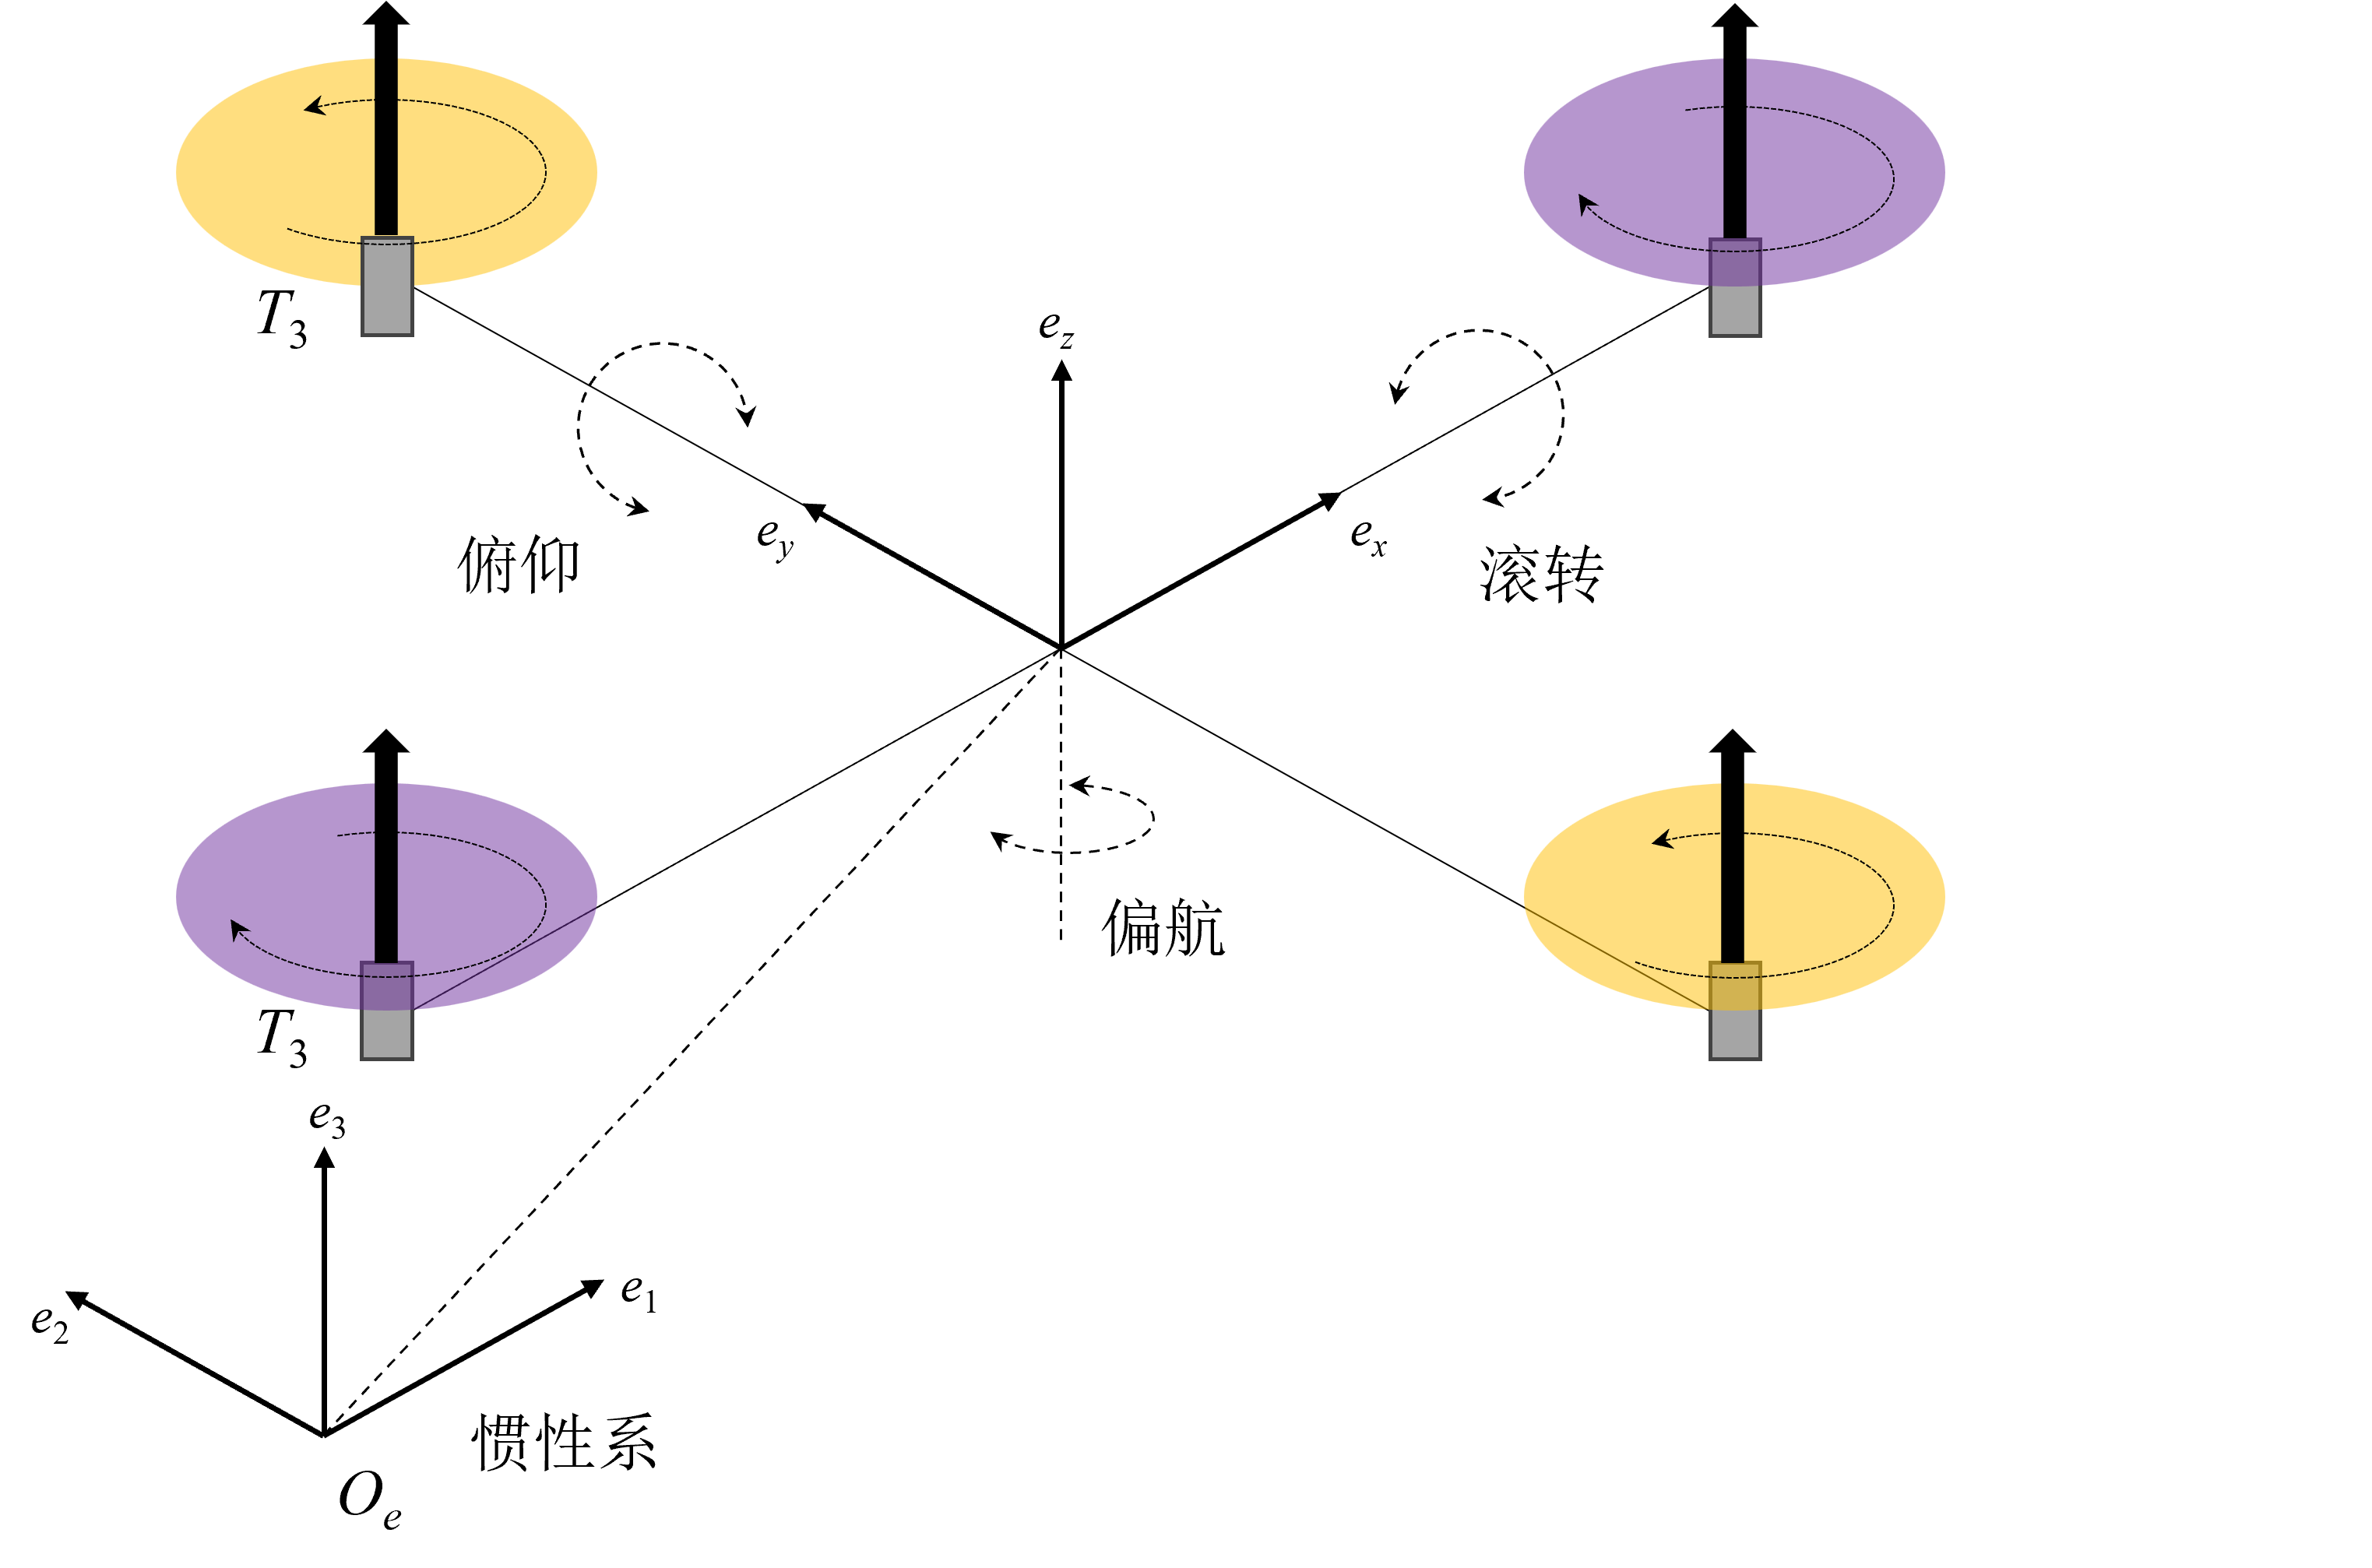
\includegraphics[width=28pc]{picture/2_1.png} 
	\caption{四旋翼无人机动力学结构} \label{2_1}
\end{figure}


对于四旋翼无人机的上升和下降,可以通过同时增加或减小电机$T_1$、$T_2$、$T_3$和$T_4$的转速来实现;滚转是四旋翼无人机通过向左或向右倾斜,以允许侧向移动的运动;俯仰是指四旋翼无人机通过前倾或后仰,向前或向后运动;偏航是指在与地面保持水平的情况下,以顺时针或逆时针的方式改变四旋翼无人机的方向。四旋翼无人机通过控制四个电机的转速,可以完成不同的飞行作业。本章根据四旋翼无人机的动力学特性建立数学模型,为下面章节控制器的设计奠定基础。


\subsection{四旋翼无人机的坐标系}
为了便于建模和描述,首先引入两个右手直角坐标系的定义,并给出两个坐标系之间的转换关系。
\subsubsection{地面坐标系}
地面坐标系$o_ex_ey_ez_e$用于研究四旋翼无人机相对于地面的运动状态,确定机体的三维位置。一般来说,在地面坐标系中,常用的局部坐标系统有 NED(North-East-Down)和ENU(East-North-Up)两种。NED坐标系$o_ex_e$轴指向正北,$o_ey_e$轴指向正东,$o_ez_e$轴垂直于地面向下。ENU坐标系 $o_ex_e$ 轴指向正东,
$o_ey_e$ 轴指向正北,$o_ez_e$ 轴垂直向上,即指向天空的方向。NED 坐标系适合飞行器或船舶等需要考虑垂直下降的系统;而ENU 坐标系更直观,符合日常地理方向的习惯,常用于地面交通、测量和定位。本文使用NED坐标系,坐标原点选择在固连于地面的任意一点。

\subsubsection{机体坐标系}
本文的四旋翼无人机为“X”型气动布局结构,运动更加灵活。
机体坐标系固连于四旋翼无人机,其原点取在四旋翼无人机的重心位置。$o_bx_b$轴在四旋翼无人机对称平面内指向机头。 $o_bz_b$轴在四旋翼无人机对称平面内,垂直轴向下。$o_by_b$轴按右手定则进行确定。机体坐标系与无人机固定连接,构成一个随四旋翼无人机运动的动坐标系。
\subsubsection{地面坐标系与机体坐标系之间的转换关系}
地面坐标系和机体坐标系的转换在无人机导航与控制中发挥着至关重要的作用。它可以帮助我们理解无人机在空间中的位置和姿态,同时实现精确的导航与控制。地面坐标系与机体坐标系之间的转换关系可以通过三个旋转矩阵来描述。具体来说,可以将地面坐标系依次沿机体坐标系进行旋转,即绕$z_b$轴旋转偏航角$\psi$,绕$y_b$旋转俯仰角$\theta$,绕$x_b$旋转滚转角$\phi$。对应的三个旋转矩阵$\boldsymbol{R}_\psi$、$\boldsymbol{R}_\theta$和$\boldsymbol{R}_\phi$分别为:
$$
\boldsymbol{R}_\psi=\begin{bmatrix}\cos\psi&-\sin\psi&0\\sin\psi&\cos\psi&0\\0&0&1\end{bmatrix} $$
$$	\boldsymbol{R}_\theta=\begin{bmatrix}\cos\theta&0&\sin\theta\\0&1&0\\-\sin\theta&0&\cos\theta\end{bmatrix} $$
$$\boldsymbol{R}_\phi=\begin{bmatrix}1&0&0\\0&\cos\phi&\sin\phi\\0&-\sin\phi&\cos\phi\end{bmatrix}
$$

因此,通过上述三个旋转矩阵,可以得到将任意矢量从地面坐标系转换到机体坐标系的转换矩阵为:
$$\begin{aligned}\boldsymbol{R}_{e-b}&=\boldsymbol{R}_{\psi}\boldsymbol{R}_{\theta}\boldsymbol{R}_{\phi}\\&=\begin{bmatrix}\cos\theta\cos\psi&\cos\theta\cos\psi&-\sin\theta\\\sin\phi\sin\theta\cos\psi-\cos\phi\sin\psi&\sin\phi\sin\theta\sin\psi+\cos\phi\cos\psi&\sin\phi\cos\theta\\\cos\phi\sin\theta\cos\psi+\sin\phi\sin\psi&\cos\phi\sin\theta\sin\psi-\sin\phi\cos\psi&\cos\phi\cos\theta\end{bmatrix}\end{aligned}$$

从机体坐标系到地面坐标系的转换矩阵为:
$$\begin{aligned}\boldsymbol{R}_{b-e}&=\bm{R}_{e-b}^\mathrm{T}\\&=\begin{bmatrix}\cos\theta\cos\psi&\sin\phi\sin\theta\cos\psi-\cos\phi\sin\psi&\cos\phi\sin\theta\cos\psi+\sin\phi\sin\psi\\\cos\theta\cos\psi&\sin\phi\sin\theta\sin\psi+\cos\phi\cos\psi&\cos\phi\sin\theta\sin\psi-\sin\phi\cos\psi\\-\sin\theta&\sin\phi\cos\theta&\cos\phi\cos\theta\end{bmatrix}\end{aligned}$$

\subsection{四旋翼无人机的模型}
四旋翼无人机模型分为运动学模型、动力学模型和控制效率模型,动力学模型既涉及运动又涉及受力情况,与物体的质量和转动惯量相关,主要用于分析无人机的受力对无人机运动速度的影响,输入为无人机旋翼产生的拉力和力矩,输出为无人机的速度和角速度。运动学模型与质量和受力无关,主要分析无人机速度对无人机位置变化产生的影响,输入为速度和角速度,输出为无人机的位置和姿态。控制效率模型输入为螺旋桨转速,输出为拉力和力矩,当已知螺旋桨转速时,可以通过控制效率模型计算出拉力和力矩。

为了简便,在对四旋翼无人机进行建模时,做了如下假设:

(1)四旋翼无人机是刚体结构,没有内力,飞行时结构无形变;

(2)四旋翼无人机的质量、螺旋桨阻力系数和转动惯量等基础参数默认不变;

(3)四旋翼无人机总保持对称结构,其几何中心与重心位置一致;

(4)四旋翼无人机只受重力和螺旋桨拉力影响,其中重力沿$o_ez_e$轴正方向,螺旋桨拉力沿$o_bz_b$轴负方向。

运动学方程描述了无人机位置与速度以及速度和角速度之间的关系,其运动学方程可以表示为:

\begin{equation}
    \begin{aligned}
	\dot{\boldsymbol{p}}_e &= \boldsymbol{v}_e = \bm{R}_{b-e} \bm{v}_b \\
	\bm{\Theta}_e &= \bm{W}_{b-e} * \bm{\omega}_b
\end{aligned}\label{2-1}
\end{equation}
其中,$\boldsymbol{p}_e=\left[x,y,z\right]^\mathrm{T}$为无人机在地面坐标系下的位置坐标,$\boldsymbol{v}_e=\left[v_{x},v_{y},v_{z}\right]^\mathrm{T}$为无人机在地面坐标系下的线速度,$\boldsymbol{v}_b=\left[u,v,w\right]^\mathrm{T}$表示无人机在机体坐标系下的线速度,$u$、$v$、$w$表示分别沿$x$、
$y$、$z$机体坐标轴方向的线速度分量,$\boldsymbol{R}_{b-e}$为上一小节定义的转换矩阵,$\bm{\Theta}_e=\left[\phi,\theta,\psi\right]^\mathrm{T}$表示无人机在地面坐标系下的姿态角度,$\bm{W}_{b-e}$表示地面坐标系下欧拉角速度变换到机体旋转角速度的旋转矩阵,$\boldsymbol{\omega}_b=\left[{\omega}_{xb},{\omega}_{yb},{\omega}_{zb}\right]^\mathrm{T}$ 为无人机机体坐标系下的角速度,可以得到姿态旋转矩阵具体形式如式(\ref{2-2})所示:
\begin{equation}
	\boldsymbol{\omega}_b=\begin{bmatrix}\omega_{xb}\\\omega_{yb}\\\omega_{zb}\end{bmatrix}=\begin{bmatrix}1&0&-\sin\theta\\0&\cos\phi&\cos\theta\sin\phi\\0&-\sin\phi&\cos\theta\cos\phi\end{bmatrix}\begin{bmatrix}\dot\phi\\\dot\theta\\\dot\psi\end{bmatrix}
	\label{2-2}
\end{equation}



一般来说,四旋翼无人机飞行时其姿态角在小范围内运动,可以近似认为有下式成立:
\begin{equation}
	\boldsymbol{\omega}_b=\begin{bmatrix}{\omega}_x\\{\omega}_y\\{\omega}_z\end{bmatrix}=\begin{bmatrix}\dot{\phi}\\\dot{\theta}\\\dot{\psi}\end{bmatrix}
	\label{2-3}
\end{equation}

以上详细描述了四旋翼无人机系统的运动学模型以及其在不同坐标系下的位置与线速度、角度与角速度之间的转换关系。接下来,将无人机整体视为一个刚体,将其分解为平移运动和旋转运动两个部分。通过牛顿法分析其平移运动,通过欧拉法分析其旋转运动,从而构建其动力学模型。其动力学的基本方程如式(\ref{2-4})所示:
\begin{equation}
	\begin{aligned}
		m\dot{\boldsymbol{v}}_e&=mg\bm{e}_{3}-\boldsymbol{R}_{b-e}f\bm{e}_{3}\\
		\boldsymbol{J}\dot{\boldsymbol{\omega}_b}&=-\bm \omega_b \times \bm J \bm \omega_b+\boldsymbol{\tau}
	\end{aligned}\label{2-4}
\end{equation}
其中$m$为无人机的质量,$g\in\mathbb{R}_+$为重力加速度,$\bm{e_{3}}=\left[0,0,1\right]^\mathrm{T}$,$\boldsymbol{\tau}=\left[\tau_x,\tau_y,\tau_z\right]^\mathrm{T}$表示无人机四个螺旋桨产生的扭矩,$\boldsymbol{J}$为无人机的惯量矩阵,$f\in\mathbb{R}_+\cup\{0\}$表示无人机螺旋桨总拉力的大小,该拉力是单向的,其形式如式 (\ref{2-5})所示:
\begin{equation}
	f=\sum_{i=1}^4f_i=c_\mathrm{T}\Omega_i^2
	\label{2-5}
\end{equation}
其中$f_i$表示表示一个旋翼在机体坐标系下旋转产生的升力,与旋翼的转速的平方正相关。$c_\mathrm{T}=1/4\pi^2\cdot\rho D_\mathrm{p}^4C_\mathrm{T}$为螺旋桨的升力系数,其大小与无人机自身的材质、倾斜角等因素有关,$\Omega_i$为
单个螺旋浆的旋转速度。由于本文采用“X”型气动布局,实际力臂长度是机臂长度的$\sqrt{2}/2$倍,可以得到无人机每个螺旋桨产生的力矩如式(\ref{2-6})所示:


\begin{equation}
	\left\{ \begin{array}{l}
		\tau_x={\sqrt{2}}/{2}dc_\mathrm{T}\left(\Omega_1-\Omega_2-\Omega_3+\Omega_4\right)\\
		\tau_y={\sqrt{2}}/{2}dc_\mathrm{T}\left(\Omega_1+\Omega_2-\Omega_3-\Omega_4\right)\\
		\tau_z=c_\mathrm{M}\left(\Omega_1-\Omega_2+\Omega_3-\Omega_4\right)\\
	\end{array} \right.
		\label{2-6}
\end{equation}
其中$c_M$为螺旋桨的反扭力系数,其产生的力矩方向沿$z$轴方向。$d\in\mathbb{R}_+$为无人机重心和任一电机转动轴线之间的距离。为了能够对应控制器中的控制量,定义虚拟控制变量为$\bm{U}=\left[U_1,U_2,U_3,U_4\right]^\mathrm{T}=\left[f,\tau_x,\tau_y,\tau_z\right]^\mathrm{T}$,那么,将式(\ref{2-2})、(\ref{2-3})、(\ref{2-5})、(\ref{2-6})代入式(\ref{2-1})和(\ref{2-4})中,即可得到四旋翼无人机的控制模型:


\begin{equation}
		\left\{
	\begin{aligned}
		&\dot{x}=v_{x}\\
		&\dot{y}=v_{y}\\
		&\dot{z}=v_{z}\\
		&\ddot{x}=\frac{U_{1}}{m}\left(\cos\phi\cos\psi\sin\theta+\sin\phi\sin\psi\right)\\
		&\ddot{y}=\frac{U_{1}}{m}\left(\cos\phi\sin\psi\sin\theta-\cos\psi\sin\phi\right)\\
		&\ddot{z}=\frac{U_{1}}{m}\left(\cos\phi\cos\theta\right)-g\\
		&\dot{\phi}={\omega}_x+\tan\theta\left({\omega}_y\sin\phi+{\omega}_z\cos\phi\right)\\
		&\dot{\theta}={\omega}_y\cos\phi-{\omega}_z\sin\phi\\
		&\dot{\psi}=\frac{{\omega}_y\sin\phi+{\omega}_z\cos\phi}{\cos\theta}\\
		&\ddot{\phi}=\frac{(I_{y}-I_{z})\cdot \dot{\theta}\dot{\psi}+U_{2}}{I_{x}}\\
		&\ddot{\theta}=\frac{(I_{z}-I_{x})\cdot \dot{\phi}\dot{\psi}+U_{3}}{I_{y}}\\
		&\ddot{\psi}=\frac{(I_{x}-I_{y})\cdot \dot{\phi}\dot{\theta}+U_{4}}{I_{z}}\end{aligned}
	\right.
	\label{2-7}
\end{equation}
\subsection{四旋翼无人机绳系吊运系统的动力学模型}
在本文的吊装运输场景中,四旋翼无人机在满足自身飞行需求的同时,还会受到吊装载荷对其作用的拉力干扰,单无人机吊装载荷受力分析如图 \ref{2_2} 所示,其中$F$表示无人机的升力,$G$表示无人机自身的重力,$G_0$表示无人机自身的重力,$T$表示载荷对无人机产生的拉力,$\theta$表示系绳与垂直平面之间的夹角。
\begin{figure}[hbt!]
	\centering
	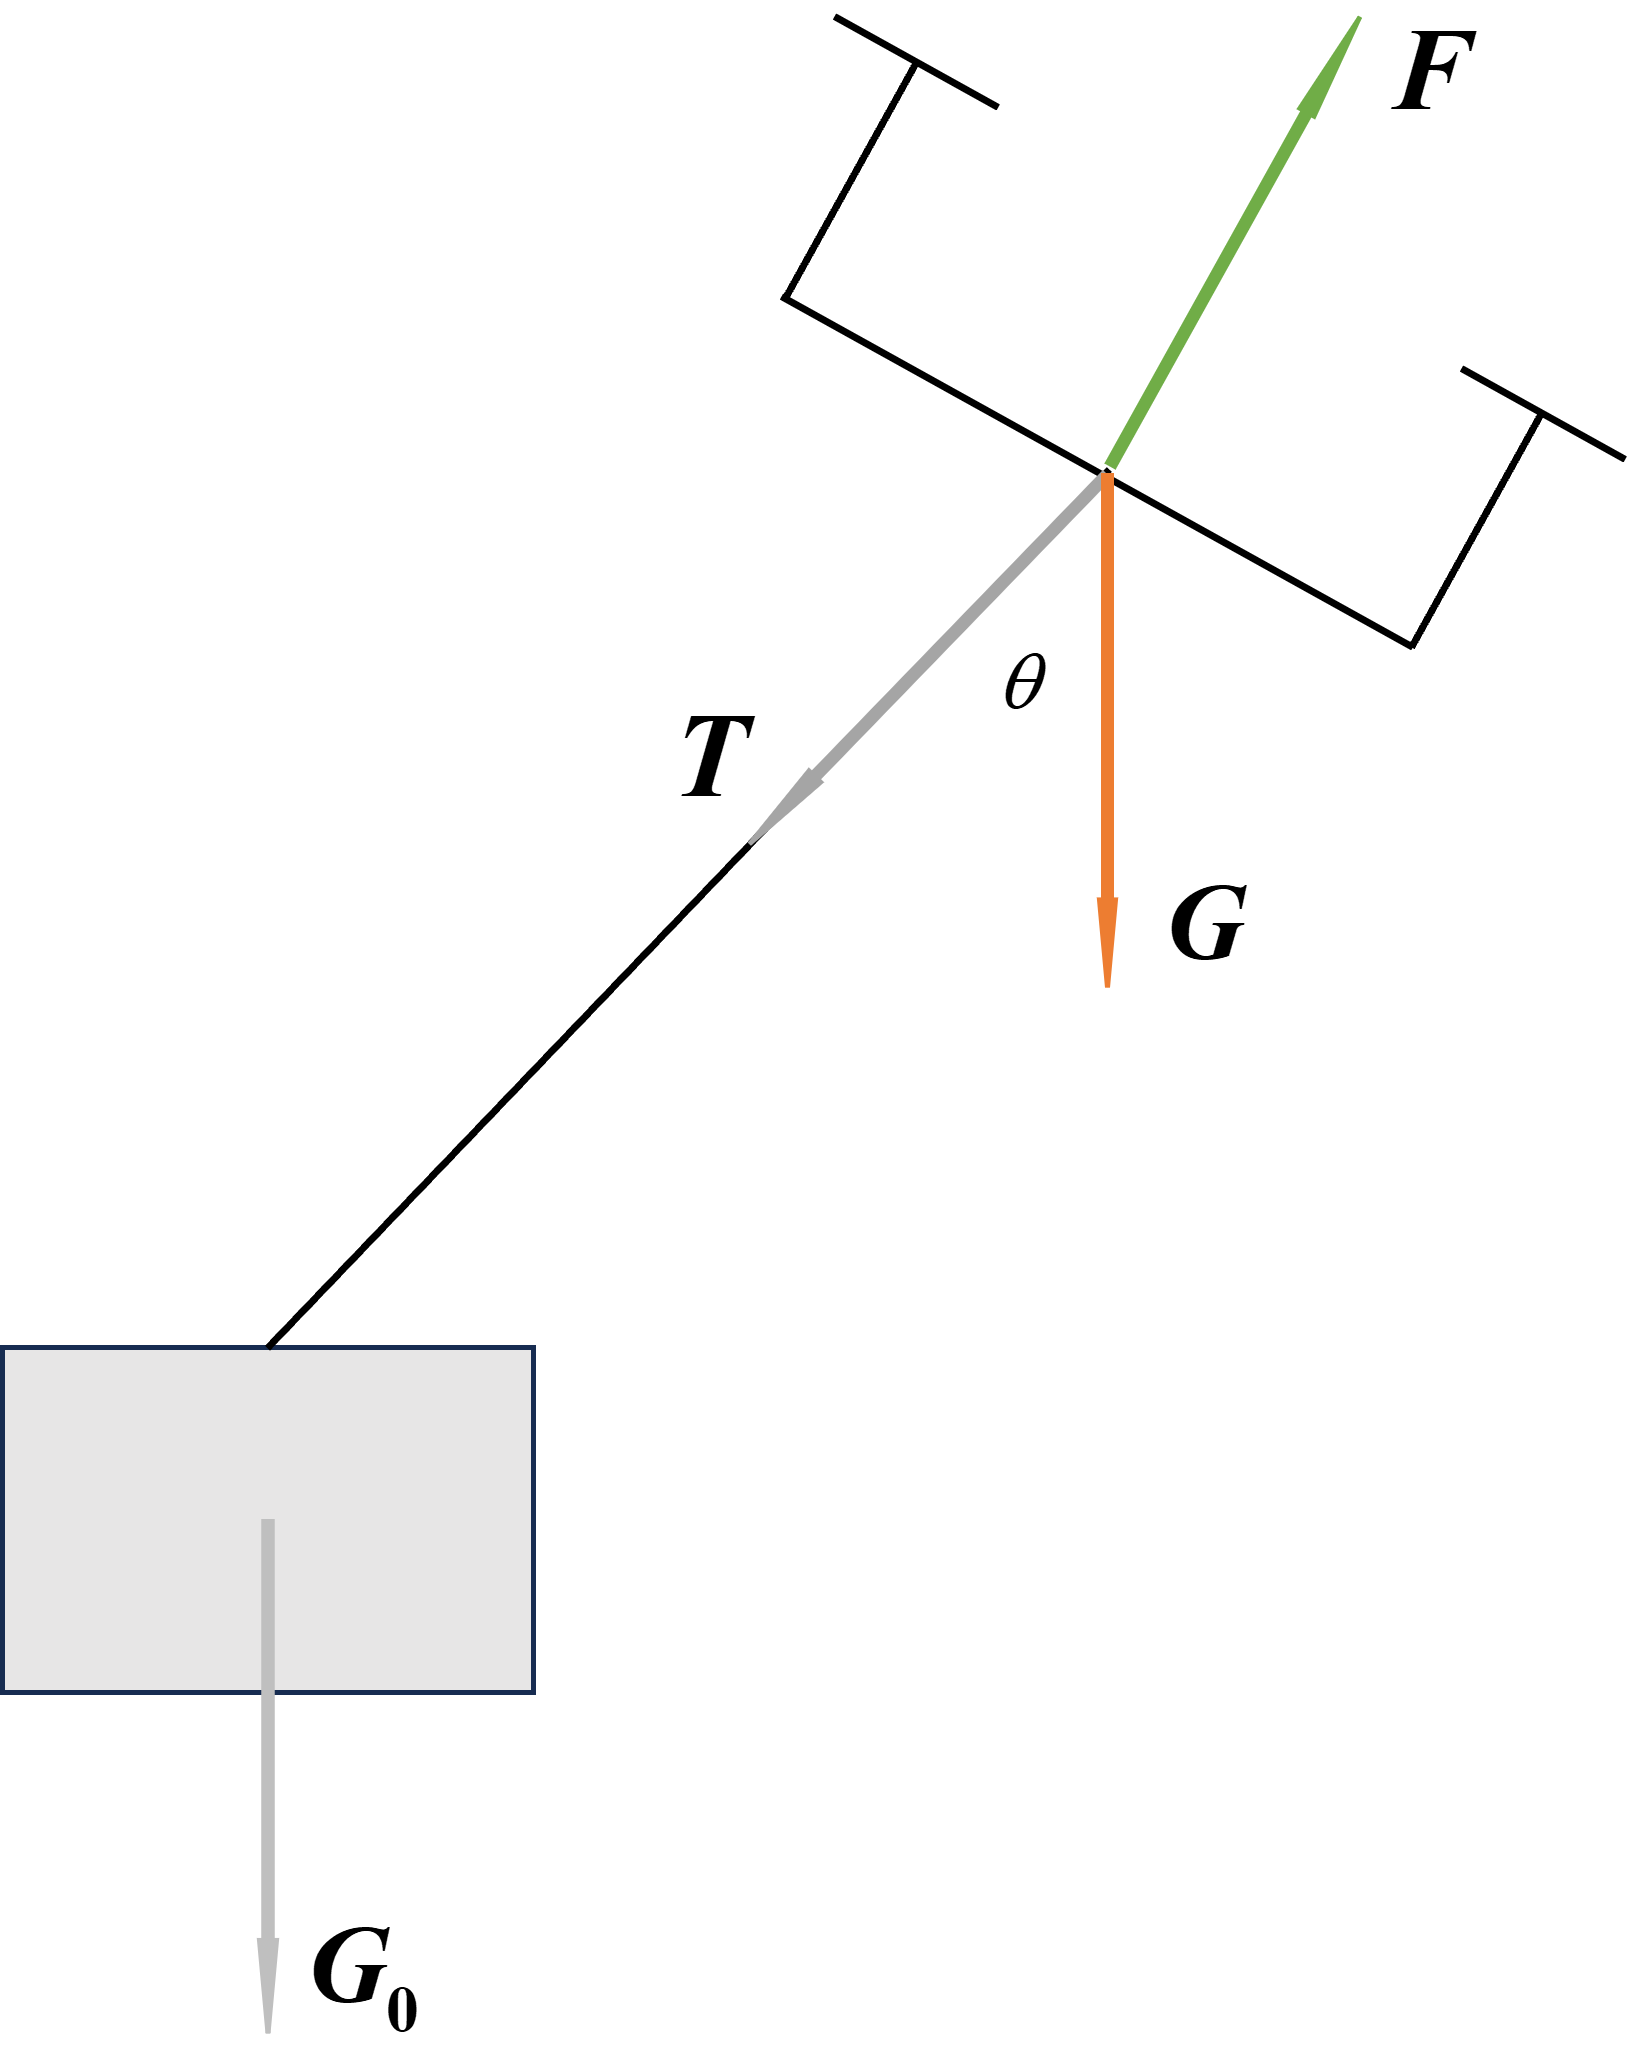
\includegraphics[width=21pc]{picture/2_2.png} 
	\caption{单无人机吊装载荷受力分析} \label{2_2}
\end{figure}

在推导对四旋翼无人机绳系吊运系统的动力学模型之前,先做了如下假设:

(1)多无人机协同吊装系统所吊挂的载荷被视为刚体; 

(2)无人机的姿态角不超过$\pi/2$;

 
通过以上假设对系统的模型进行了简化,使得任务更合理。对于四旋翼无人机绳系吊运系统来说,在轨迹跟踪时其系绳并不一定总是保持绷直状态的,在无人机的高速移动中系绳上的张力可能为零。因此,本文建立四旋翼无人机绳系吊运系统的混合模型,考虑系绳上的张力不为零和张力为零这两种情况。

\subsubsection{系绳张力不为零时的动力学模型}

四旋翼无人机绳系吊运系统由载荷相对于地面坐标系的位置、载荷姿态和四旋翼飞行器的姿态来定义。当系绳拉紧时,该系统具有八个自由度,并存在四个自由度的欠驱动。四旋翼无人机和载荷的位置之间的关系为:

\begin{equation}
	\bm p_Q=\bm p_L-l\bm q
\end{equation}
其中$\bm p_Q$、$\bm p_L$分别为四旋翼无人机和载荷的位置,$l$为系绳的长度,$\bm q$表示从四旋翼无人机指向载荷的单位向量。本文采用拉格朗日法来推导运动方程。系统的拉氏量 $\mathcal{L}:T\bar{Q}\to\mathbb{R}$ 定义为$\mathcal{L}=\mathcal{T}-\mathcal{U}$,其中$\mathcal{T}:TQ\to\mathbb{R}$和${\mathcal{U}}:Q\to\mathbb{R}$分别是机械系统的动能和势能,它们的定义如下:

\begin{equation}
\begin{aligned}
	\mathcal{T}=\frac{1}{2}&m_{Q}\bm v_{Q}\cdot \bm v_{Q}+\frac{1}{2}m_{L}\bm v_{L}\cdot \bm v_{L}+\frac{1}{2}\langle\hat{\bm  \omega_Q},\widehat{\bm J_{Q}\bm  \omega_Q}\rangle\\
	&\mathcal{U}=m_{Q}g\bm e_{3}\cdot \bm x_{Q}+m_{L}g\bm e_{3}\cdot \bm x_{L}
\end{aligned}
	\label{2-8}
\end{equation}
其中$\bm v_Q$、$\bm v_L$分别为无人机和载荷的速度,$m_Q$、$m_L$分别为无人机和载荷的质量,$\langle\cdot,\cdot\rangle $表示内积,$\hat{.}$被定义为使得 $\hat{\bm x}\bm y=\bm x\times \bm y$对于所有$\bm x,\bm y\in\mathbb{R}^3$恒成立,$\omega_Q$为四旋翼飞行器在机体坐标系下的角速度。在本文中,$\lambda_m(\cdot)$和 $\lambda_n(\cdot)$ 分别表示矩阵的最小和最大特征值。系统的动力学满足拉格朗日原理:
\begin{equation}
	\bm \delta\int_0^\tau\mathcal{L} dt+\int_0^\tau\left(\langle \bm W_1,\hat{\bm \tau}\rangle+\bm W_2\cdot f\bm{R}_{b-e}\bm e_3\right) dt=0
	\label{2-10}
\end{equation}
其中$\bm W_{1}=\bm R_{b-e}^{T}\bm \delta \bm R_{b-e}$是定义在旋转空间上的变分向量场, $ \bm W_{2}=\bm \delta \bm x_{Q}=\bm \delta \bm x_{L}-l\bm \delta q$是定义在平移空间上的变分向量场,两者共同描述刚体系统中的变分动态,并且满足以下条件:
\begin{equation}
	\begin{aligned}
	&\bm \delta \bm q = \bm \xi \times \bm q\\
	\bm \delta \dot{\bm q} = &\dot{\bm \xi} \times \bm q + \bm \xi \times \dot{\bm q} \\
	\bm \delta\bm  R&_{b-e} = \bm R_{b-e} \hat{\bm \eta} \\
	\bm \delta \hat{\bm  \omega _Q}& = \widehat{\hat{\bm  \omega_Q} \bm \eta} + \hat{\dot{\bm \eta}}
\end{aligned}
\end{equation}
其中$\bm \delta \bm q$为二维球面上的变分,$\bm \delta \bm R$为三维空间上的变分。
向量 $\bm{\xi} \in \mathbb{R}^3$ 是一个三维实数向量,满足 $\bm{\xi}$ 与向量 $\bm{q}$ 的点积为零,即$\bm{\xi}$ 垂直于 $\bm{q}$,向量 $\bm{\eta} \in \mathbb{R}^3$ 是一个三维实数向量。

由于(\ref{2-10})对所有可能的变化都是满足的,因此得到带有系绳载荷的四旋翼无人机的运动方程为:

\begin{equation}
	\begin{aligned}
		&\dot{\bm x}_{L}=\bm v_{L} \\
		(m_Q+m_L)(\dot{\bm v}_L+g\bm e_3)& =(\bm q\cdot f\bm R\bm e_3-m_Ql(\dot{\bm q}\cdot\dot{\bm q}))\bm q \\
		&\dot{\bm q}=\bm \omega_L\times \bm q \\
		m_{Q}l \dot{\bm \omega_L}&=-\bm q\times f\bm R\bm e_{3} \\
		&\dot{\bm R_{b-e}}=\bm R_{b-e}\hat{\bm  \omega_Q} \\
		\bm J_{Q}\dot{\bm  \omega_Q}+&\bm  \omega_Q\times \bm J_{Q}\bm  \omega_Q=\bm \tau
	\end{aligned}
\end{equation}

上述动力学可以写成标准形式 $\dot{\bm X}_n=\bm f_n(\bm X_n)+\bm g_n(\bm X_n)\bm u$ ,其中 $\bm X_n = \{\bm x_L,\bm q,\bm R_{b-e},\bm v_L,\bm \omega_L,\bm \omega_Q\}$ 是系统的状态,$\bm u = \left[f,\bm \tau \right]$是系统的输入。
\subsubsection{系绳张力为零时的动力学模型}
当系绳张力趋于零时,四旋翼飞行器和吊挂载荷作为独立系统,载荷处于自由落体状态。在这种情况下,四旋翼无人机绳系吊运系统的运动方程为:
\begin{equation}
	\begin{aligned}
	&\dot{\bm x}_{L}=\bm v_{L}\\
	\quad m_{L}(&\dot{\bm v}_{L}+g\bm e_{3})=0\\
	&\dot{\bm x}_{Q}=\bm v_{Q}\\
	\quad m_{Q}(\dot{\bm v}_{Q}&+g\bm e_{3})=f\bm R_{b-e}\bm e_{3}\\
	&\dot{\bm R_{b-e}}=\bm R_{b-e}\hat{\Omega}\\
	\quad \bm J_{Q}\dot{\bm \Omega}+&\bm \Omega\times \bm J_{Q}\bm \Omega=\bm \tau
\end{aligned}
\end{equation}
上述方程也可以写成标准形式$\dot{\bm X}_n=\bm f_n(\bm X_n)+\bm g_n(\bm X_n)\bm u$,其中中$\bm X_n = \{\bm x_L,\bm x_Q,\bm R_{b-e},\bm v_L,\bm v_Q,\bm \omega_b\}$为状态。

\subsubsection{混合系统的动力学模型}
系绳悬挂载荷的四旋翼飞行器是一个混合系统,因为当缆索中的张力降为零或当张力恢复时松弛的缆索变得绷紧时,动力学会发生切换。混合模型可以写成,
\begin{equation}
	\left.\begin{aligned}&\Sigma_{n}:\left\{\begin{array}{ll}\dot{\bm X_n}=\bm f_n(\bm X_n)+\bm g_n(\bm X_n)\bm u  &\bm X_n\notin \mathbb{S}_z\\\bm X_z^+=\Delta_{n\to z}(\bm X_n^-)  &\bm X_n\in \mathbb{S}_z\end{array}\right.\\&\Sigma_{z}:\left\{\begin{array}{ll}\dot{\bm X_z}=\bm f_z(\bm X_z)+\bm g_z(\bm X_z)\bm u \ \ &\bm X_z\notin \mathbb{S}_n\\\bm X_n^+=\Delta_{z\to n}(\bm X_z^-) \ &\bm X_z\in \mathbb{S}_n\end{array}\right.\end{aligned}\right.
\end{equation}
其中集合$\mathbb S_z = \{ \bm X_n \mid  T \equiv 0 \}$,$\mathbb S_n = \{ \bm X_z \mid \|\bm x_Q - \bm x_L\| \equiv l, d \|\bm x_Q - \bm x_L\| /dt> 0 \}$,系绳上的张力定义为$T = \|m_L (\ddot{\bm x}_L + g\mathbf{e}_3)\|$,状态转移映射$\Delta_{n\to z}$为单位映射,$\Delta_{z\to n}$为两个物体非弹性碰撞的模拟,并满足条件$\dot{\bm x}_Q^+-\dot{\bm x}_L^+=0$。

\section{多无人机绳系吊运系统的动力学模型}
在本文中,我们采用三个无人机吊挂载荷的方式来运输载荷。该吊运系统
由三个四旋翼无人机、三根绳索和一个需要被运输的重物组成。其吊运结构如图 \ref{2_3} 所示,三架无人机保持水平高度一致,无人机之间的相对距离为$d$。为建
立多机吊运系统的动力学模型,本章采用了两个坐标系,即惯性坐标系和机体
坐标系。


基于以下几个假设条件对三机吊运系统进行动力学建模:
(1)四旋翼无人机是一个刚体模型,有效载荷被视为一个质点;
(2)连接无人机与有效载荷之间的绳索为无弹性绳索,且质量可忽略;
(3)不考虑空气阻力等环境扰动。
在多无人机吊挂载荷运输系统中,对四旋翼无人机进行受力分析,与单机
模型相比不同的是,吊运无人机承受了额外的绳子拉力,因此其运动学和动力学模型表达式为:

\begin{equation}
	\begin{cases}{}^{e}\dot{\boldsymbol{p}}={}^{e}\boldsymbol{v}\\{}^{e}\dot{\boldsymbol{v}}=-g\boldsymbol{e}_{3}+\frac{f_{T}}{m}\boldsymbol{R}_{b}^{e}\boldsymbol{e}_{3}-\frac{f_{L}}{m}\\\dot{\boldsymbol{\Theta}}=\boldsymbol{W}\cdot^{b}\boldsymbol{\omega}\\\boldsymbol{J}\cdot^{b}\dot{\boldsymbol{\omega}}+^{b}\boldsymbol{\omega}\times(\boldsymbol{J}\cdot^{b}\boldsymbol{\omega})=\boldsymbol{\tau}+\boldsymbol{\tau}_{L}\end{cases}
\end{equation}

其中$f_{L}=[f_{L_{-}x},f_{L_{-}y},f_{L_{-}z}]^{\mathrm{T}}$表示惯性系下绳子产生的拉力向量。$\tau_{L}$表示绳子拉力对四旋翼无人机机体产生的力矩向量。

在惯性坐标系下,载荷位置向量为$p_{l}=[p_{lx},p_{ly},p_{lz}]^{\mathrm{T}}$,三个无人机的位置向
量分别用$p_{q1}$、$p_{q2}$、$p_{q3}$来表示,吊绳长度为$L$。对悬吊的载荷进行受力分析,由牛顿第二定律可得出:
\begin{equation}
	\begin{aligned}
		&f_{Li}=\frac{1}{L}(p_{qi}-p_{l})T_{i} \\
		&m_{1}\ddot{p}_{1}=-m_{1}ge_{3}+\sum_{i=1}^{3}f_{Li}
	\end{aligned}
\end{equation}
其中$f_{Li}$表示第i根绳子在惯性坐标系下所提供的拉力向量;$T_{i}$表示第$i$根绳子提供的拉力值标量。

\begin{figure}[hbt!]
	\centering
	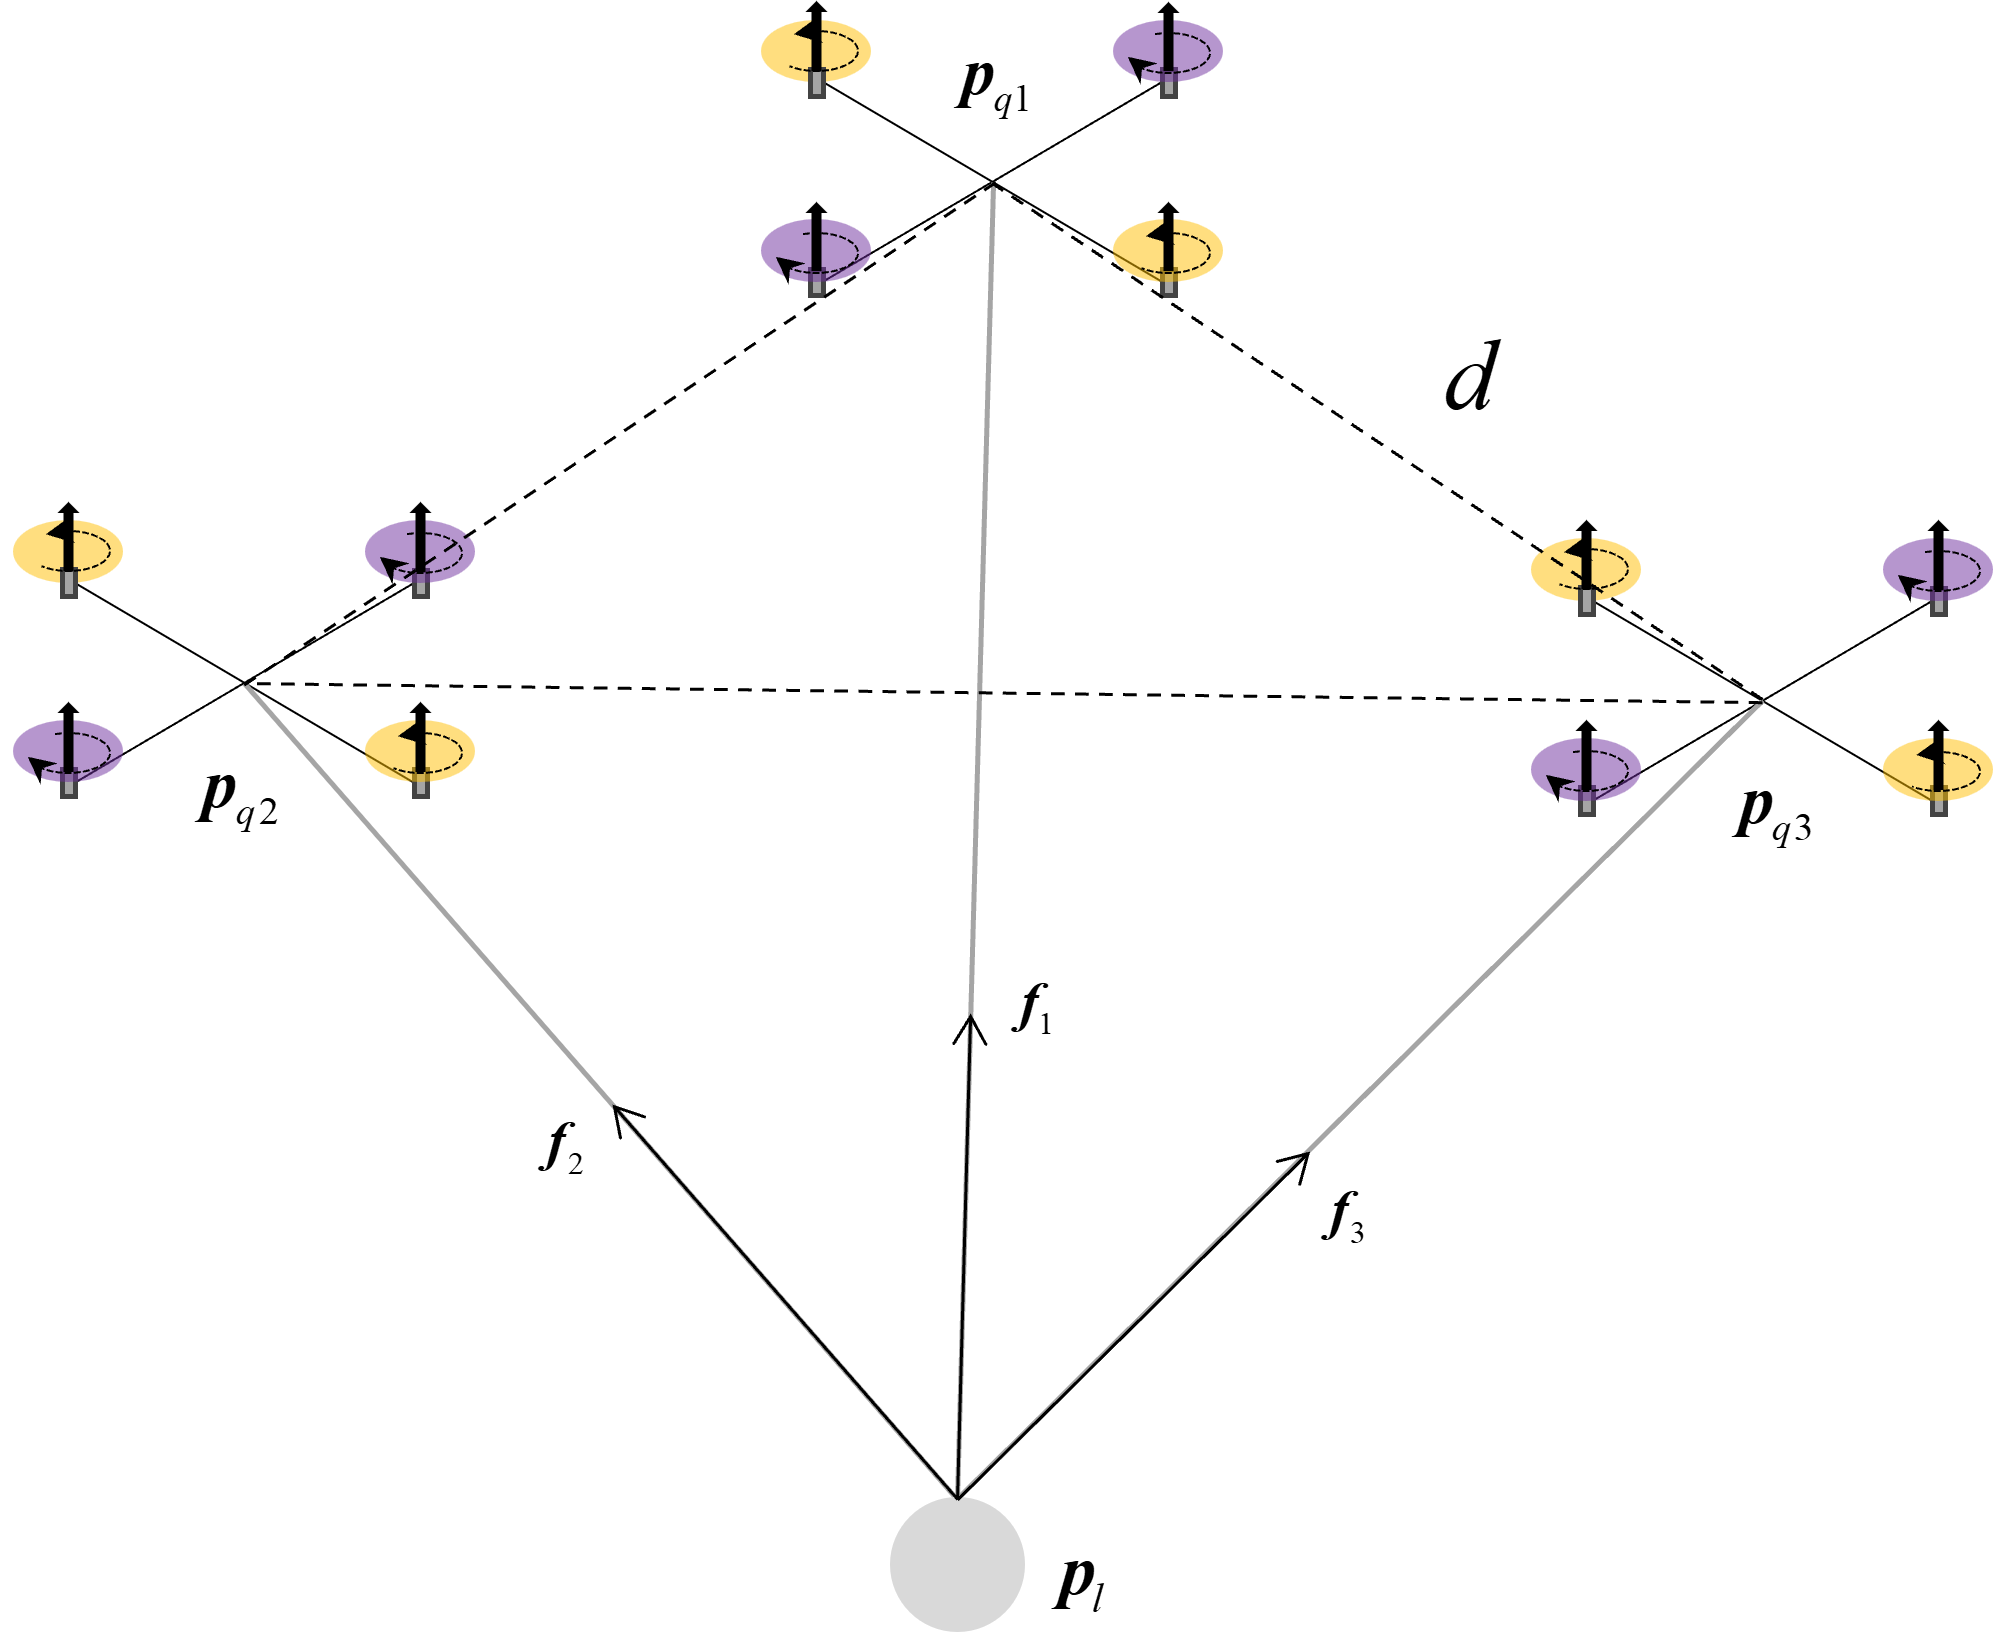
\includegraphics[width=23pc]{picture/2_3.png} 
	\caption{多无人机吊运系统} \label{2_3}
\end{figure}

\section{本章总结}

\cleardoublepage

\chapter{单无人机吊运控制}
\chaptermark{单无人机吊运控制}

许多学者都关注了单个无人机的控制问题,但是对于单个无人机搬运的控制问题,尤其是高精度跟踪控制问题比较难处理,再加上本文还有无人机搬运的载荷也会对无人机产生影响,所以本章考虑对载荷的精确位置跟踪控制问题。本章的任务是对无人机设计控制器,使得载荷能够跟踪指定的参考路径运动。 

本文把载荷当成一种干扰,首先用干扰观测器把载荷对无人机外环和内环的影响估计出来,然后在所设计的控制器中将该干扰进行补偿,这样所设计的控制器可以消除干扰对系统的影响,从而提高无人机搬运载荷的控制精度。

\section{问题描述}
在第 2 章中,我们介绍了单无人机绳系吊运系统的动力学模型,并建立了系绳上张力为零和不为零这两种情况组成的混合模型,该模型需要考虑两种情况之间的切换过程,然而对于控制器来说,载荷的状态信息是难以直接进行获取的。因此,本章采用数据驱动的方法,将动力学模型表达式(2-26)改写成如下形式:
\begin{equation}
	\begin{aligned}
		\dot{\boldsymbol{p}}_e = \boldsymbol{v}_e, \
		\dot{\boldsymbol{v}}_e = m^{-1}\left(-mg\bm{e}_3+\boldsymbol{R}_{b-e}f\bm{e}_3+\bm{f}_p+\bm{f}_{\text{res}}\right) \\
		\dot{\bm{R}_{b-e}} = \bm{R}_{b-e} \bm{\omega}_b^{\times}, \
		\dot{\boldsymbol{\omega}}_b = \boldsymbol{J}^{-1}\left(-\bm{\omega}_b^{\times}\bm{J} \bm{\omega}_b+\boldsymbol{\tau}+ \bm{\tau}_p+ \bm{\tau}_{\text{res}}\right)
	\end{aligned}\label{3-1}
\end{equation}



其中,$\bm{f}_p$和$\bm{\tau}_p$分别为有效载荷作用在无人机上的力和扭矩,$\bm{f}_\text{res}$和$\bm{\tau}_\text{res}$分别为无人机自身产生的残余力和扭矩。
为完整起见,我们将无人机受到的有效载荷和残余力叠加到一起,当作未知的非线性项即$\bm f_e = \bm f_p+ \bm f_{\text{res}}$ 和 $\bm \tau_e = \bm \tau_p+\bm \tau_{\text{res}}$ 。
	
该动力学模型中,非线性项$\bm f_e$和$\bm \tau_e$都是动态时变函数,其与无人机和吊挂载荷的运动状态高度耦合。本章需要解决问题是使用基于数据驱动的方法学习单无人机绳系吊运系统未知的系绳和载荷模型,然后将学习到的模型用非线性项进行表示,并集成到控制器中,实现无人机对期望轨迹的准确跟踪。 




\section{Koopman算子理论}

Koopman算子理论是一种用于分析和控制非线性动力系统的强大工具。该理论的核心思想是通过将非线性系统的状态空间映射到一个更高维的线性空间,从而将非线性系统转化为线性系统进行分析和控制。具体来说,Koopman算子理论通过引入一组称为“可观测量”的函数,将原始系统的非线性状态映射到一个线性状态空间中,从而使得原本复杂的非线性系统可以用线性系统的方法进行处理。
Koopman算子理论的提出为建模方法以及模型线性化方法提供了新的思路,本章中基于数据驱动的方法使用了Koopman算子理论的思想,因此,在本小节先对Koopman算子理论进行一个简单的介绍。

\subsection{经典Koopman算子理论}

考虑一个离散时间动力系统,其状态向量 \( x \in \mathcal{X} \subseteq \mathbb{R}^{N_x} \)。系统的传播规则由非线性函数 \( T \) 表示(如图 \ref{3_1} 所示)。通过使用可观测函数 \( x \mapsto g(x) \) 将原始状态 \( x \) 提升到新的空间,系统的动力学可以在一个新空间中重新定义,其中线性算子,称为Koopman算子 \( \mathcal{K} \),描述了系统的动力学。换句话说,尽管 \( T \) 和 \( \mathcal{K} \) 作用在不同的空间上,但它们封装了相同的动态特性。例如,给定当前状态 \( x \),可以通过两种途径将其传播到下一个时间步并进行观测:要么使用 \( T \) 计算 \( T(x) \) 并观测结果状态(底部路径),要么使用可观测函数,应用 \( \mathcal{K} \) 并在 \( x \) 处进行评估(顶部路径)。这种“等价”或“替代”概念提供了几个优势:

(1)它使得非线性动力学 \( T \) 能够全局线性表示,从而使得适用于线性系统的方法得以应用。

(2)它通过实时学习线性算子来估计底层动力学,从而消除了对非线性函数进行最小二乘回归的需求,这在一般情况下需要大量数据。
\begin{figure}[hbt!]
	\centering
	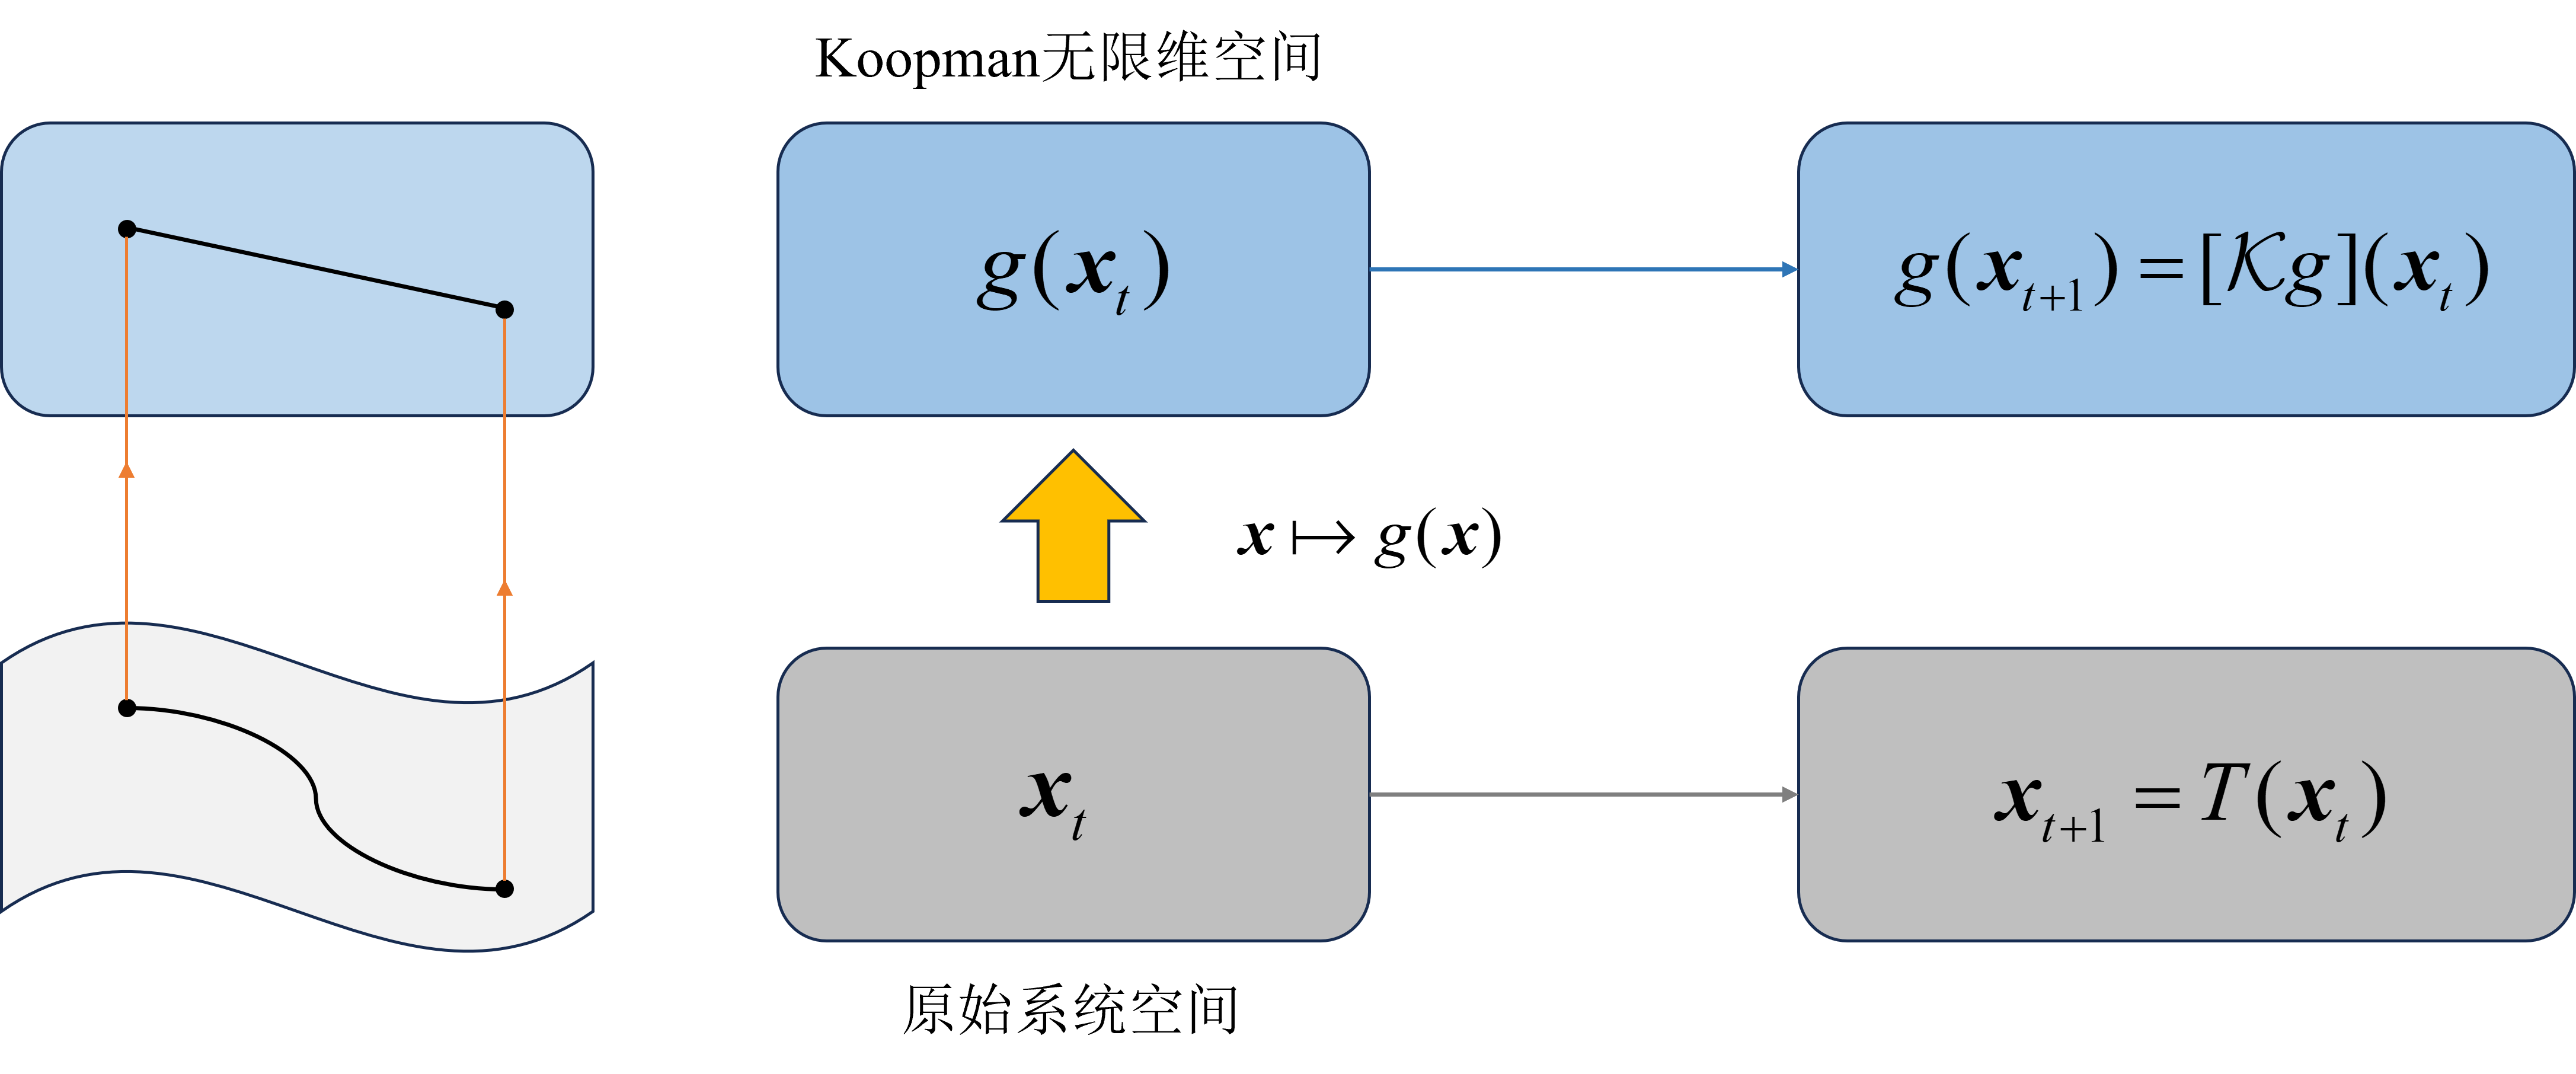
\includegraphics[width=34pc]{picture/3_1.png} 
	\caption{Koopman算子理论} \label{3_1}
\end{figure}
\subsection{基于Koopman理论的数据驱动预测}

考虑一个离散时间的动力学系统:
\begin{equation}
	x_{t+1} = T(x_t)\label{3-2}
\end{equation}

考虑一个复值函数(称为可观测量)的向量空间 \( \mathcal{F} \),其定义域为系统的状态空间。可以将可观测量 \( g \in \mathcal{F} \) 视为映射或提升的状态。使用与式(\ref{3-2})相关的Koopman算子 \( \mathcal{K}: \mathcal{F} \to \mathcal{F} \) 对可观测量 \( g \) 的演化表示为:
\begin{equation}
	\mathcal{K}g = g \circ T, \quad \forall g \in \mathcal{F}
	\label{3-3}
\end{equation}
其中 \( \circ \) 表示函数复合。为了确保 \( \mathcal{K} \) 是良定义的, \( \mathcal{F} \) 必须在 \( T \) 的复合下封闭。如果 \( \mathcal{F} \) 包含特定的预定义函数(如返回完整状态值的函数),这一条件可能迫使 \( \mathcal{F} \) 成为无限维的。Koopman算子根据以下规则将系统向前传播一步:
\begin{equation}
	\mathcal{K}g(x_t) = g \circ T(x_t) = g(T(x_t)) = g(x_{t+1})
	\label{3-4}
\end{equation}

提升状态 \( g(x) \) 本质上将原始(非线性)系统转化为在Koopman空间中演化的线性系统,从而可以设计和实现各种线性控制器(如LQR)。为了避免处理无限维空间,可以使用Koopman算子的有限维表示。因此,在Koopman算子下不变的有限维子空间 \( \mathcal{S} \subset \mathcal{F} \) 起着至关重要的作用。形式上,设 \( \mathcal{S} \subset \mathcal{F} \) 是一个有限维Koopman不变子空间,并将Koopman算子的作用限制在 \( \mathcal{S} \) 上,即 \( \mathcal{K} \rvert_\mathcal{S}: \mathcal{S} \to \mathcal{S} \)。由于 \( \mathcal{S} \) 是有限维的,给定其基,可以将其表示为矩阵。形式上,设 \( \Psi \) 是一个向量值函数,其元素构成 \( \mathcal{S} \) 的基,则存在一个矩阵 \( \mathcal{K} \in \mathbb{C}^{\text{dim}(\mathcal{S}) \times \text{dim}(\mathcal{S})} \),使得:
\begin{equation}
	\mathcal{K}\Psi = \Psi \circ T = \mathcal{K}\Psi
	\label{3-5}
\end{equation}

结合(\ref{3-5})和(\ref{3-4}),可以得到系统轨迹的线性演化,从而使得(\ref{3-2})可以使用线性系统理论的方法,即:
\begin{equation}
	\Psi(x_{t+1}) = \mathcal{K}\Psi(x_t)\label{3-6}
\end{equation}

通过定义 \( z_t := \Psi(x_t) \),(\ref{3-6})可以写成线性形式 \( z_{t+1} = \mathcal{K}z_t \)。如果空间 \( \mathcal{S} \) 包含状态可观测量 \( g_i(x) = x_i \),其中 \( x_i \) 是状态 \( x \) 的第 \( i \) 个元素,则可以选择基 \( \Psi \) 使其包含 \( g_i \) 作为其元素。在这种情况下,提升的线性系统(\ref{3-6})捕获了原始非线性系统(\ref{3-2})的完整信息。此外,矩阵 \( \mathcal{K} \) 的特征分解允许识别Koopman特征函数和特征值。

通常,找到包含所有状态可观测量的精确有限维不变子空间是具有挑战性的(有时是不可能的)。一个流行的解决方法是近似。假设空间 \( F \) 配备了内积,给定任意空间 \( \mathcal{S} \)(不一定是Koopman算子下的不变空间),可以考虑算子 \( P_\mathcal{S} \mathcal{K}: \mathcal{F} \to \mathcal{F} \),其中 \( P_\mathcal{S} \) 是 \( \mathcal{S} \) 上的正交投影算子。对于这个算子,空间 \( \mathcal{S} \) 是通过构造不变的。因此,可以将这个算子的作用限制在 \( \mathcal{S} \) 上,即 \( P_\mathcal{S} \mathcal{K} \rvert_\mathcal{S}: \mathcal{S} \to \mathcal{S} \),并给定 \( \mathcal{S} \) 的基 \( \Psi \),该算子承认矩阵表示:
\begin{equation}
	P_\mathcal{S} \mathcal{K}\Psi = \hat{\mathcal{K}}\Psi
	\label{3-7}
\end{equation}
其中 \( \hat{K} \in \mathbb{C}^{\text{dim}(\mathcal{S}) \times \text{dim}(\mathcal{S})} \)。在这种情况下,可以写出(4)的近似版本如下:
\begin{equation}
	\Psi(x_{t+1}) = [\mathcal{K}\Psi](x_t) \approx [P_\mathcal{S} K\Psi](x_t) = \hat{\mathcal{K}}\Psi(x_t)
	\label{3-8}
\end{equation}

通过定义 \( z_t := \Psi(x_t) \),前述方程可以写成近似线性形式 \( z_{t+1} \approx \hat{\mathcal{K}}z_t \),从而可以使用高效的线性方法来近似系统的行为。在实践中,通常可以访问系统的离散采样测量数据。这可以用于获得无限维Koopman算子的有限维近似矩阵以及这些基于Koopman的组件。

与标准状态空间模型不同,Koopman算子模型了由系统动力学 \( f \) 驱动的函数演化,并且其存在性对于前向完备系统是保证的。由于Koopman算子是作用在函数空间上的算子,因此它通常是无限维的,但关键在于即使动力学 \( f \) 是非线性的,Koopman算子仍然是线性的。因此,如果 \( \phi \) 是与特征值 \( \lambda \in \mathbb{C} \) 相关联的特征函数,则有 \( K\phi = \lambda\phi \)。由此可以看出,特征函数(或特征函数的线性组合)沿着非线性系统(5)的轨迹线性演化:
\begin{equation}
	\phi(x_{k+1}) = \phi(f(x_k)) = (K\phi)(x_k) = \lambda\phi(x_k)
\end{equation}

给定一组特征函数 \(\{\phi_i\}_{i=1}^{n_\phi}\),任何位于这些特征函数张成的空间内的可观测量都可以分解为:
\begin{equation}
	\psi = \sum_i c_i(\psi)\phi_i
\end{equation}
其中 \( c_k(\psi) \) 称为 \( \psi \) 的Koopman模态。于是我们有:
\begin{equation}
	K\psi = \sum_i c_i(\psi)\lambda_i\phi_i
\end{equation}
其中 \( \lambda_i \) 表示 \( \phi_i \) 的特征值。

在后续内容中,下标 \( u \) 用于表示与带有控制输入的系统相对应的组成部分。给定一个带有控制输入的非线性动力学:
\begin{equation}
	x_{k+1} = f_u(x_k, u_k)
\end{equation}

Koopman算子可以以不同的方式定义。在本工作中,我们考虑了文献[22]中的框架。具体来说,记无限控制序列 \( u := \{u_k\}_{\infty}^{k=0} \in l(U) \),其中 \( l(U) \) 表示所有控制序列的空间。增广状态为:
\begin{equation}
	\chi=\begin{bmatrix}x\\u\end{bmatrix}
\end{equation}

系统的动力学被增广为:
\begin{equation}
	F(\chi_k)=\begin{bmatrix}f_u(x_k,u_k(0))\\Su_k\end{bmatrix}
\end{equation}

其中 \( S \) 是左移算子,定义为 \( Su(i) := u(i + 1) \),且 \( u(i) \) 是 \( u \) 的第 \( i \) 个元素的值。在这种设置下,\( u \) 可以被视为从索引 \( i \) 到实际输出 \( u_i \) 的序列映射。值得注意的是,这个动力系统是无限维的但自治的。因此,上述Koopman算子的定义可以直接应用,并且相应的特征函数假设由以下基函数字典张成:
\begin{equation}
	\{\phi_u(x, u)\}_{i=1}^{n_{\phi_u} + n_u} := \{\phi_{u,1}(x), \ldots, \phi_{u,n_{\phi_u}}(x), u(0)\}
\end{equation}

如果这个基函数字典的演化在系统动力学下是封闭的,那么我们有:
\begin{equation}
\begin{aligned}
	z_{k+1}=Az_k+&Bu_k(0)\\u_{k+1}(0)=&u_k(1)
\end{aligned}
\end{equation}
其中 \( z_k := [\phi_{u,1}(x_k), \ldots, \phi_{u,n_{\phi_u}}(x_k)] \),且 \( A \) 和 \( B \) 捕获了Koopman算子。类似地,这些基函数张成的空间内的任何函数都可以通过Koopman模态恢复为:
\begin{equation}
	\psi_u(x, u(0)) = c_u^T \begin{bmatrix} z \\ u(0) \end{bmatrix}
\end{equation}
其中 \( c := [c_{u,1}, c_{u,2}, \ldots, c_{u,n_{\phi_u} + n_u}] \) 是Koopman模态的向量。特别地,我们对系统输出的恒等函数评估的Koopman模态感兴趣。假设我们有 \( n_y \) 个输出,第 \( i \) 个输出的评估为 \( I_{y,i}(y_k) := y_{k,i} \)。通过一些符号的滥用,输出评估的Koopman模态分解为:
\begin{equation}
	y_k = \begin{bmatrix} I_{y,1}(y_k) \\ I_{y,2}(y_k) \\ \vdots \\ I_{y,n_y}(y_k) \end{bmatrix} = \begin{bmatrix} c_{u,1}^T \\ c_{u,2}^T \\ \vdots \\ c_{u,n_y}^T \end{bmatrix} \begin{bmatrix} z \\ u(0) \end{bmatrix} := C_u \begin{bmatrix} z \\ u(0) \end{bmatrix}
\end{equation}
其中 \( C_u \) 堆叠了输出评估的Koopman模态。

总之,Koopman算子理论通过将非线性系统提升到更高维的线性空间,使得复杂的非线性控制问题可以用线性方法进行处理,从而为非线性系统的控制设计提供了一种有效的工具。

\section{模型预测控制方法}

本小节重点阐述模型预测控制(Model Predictive Control,简称MPC)的基本原理及其应用流程,结合鲁棒非线性控制方法和离散化建模,形成适用于四旋翼无人机系统的完整设计框架。从预测模型建立到代价函数设计,再到优化问题求解,MPC为复杂控制问题提供了一种系统化、灵活性强的解决方案。通过系统状态的预测、滚动优化与反馈修正的有机结合,MPC方法在应对系统非线性、不确定性和外部扰动方面表现出显著的优势。


模型预测控制的核心思想是利用系统的数学模型预测未来的动态行为,并通过在线求解优化问题生成控制输入。其主要特性包括:

(1)预测与滚动优化:通过预测系统在未来一段时间内的行为,寻找最优的控制输入序列;仅执行最优序列中的首个输入,并滚动更新预测区间。

(2) 反馈矫正:实时采集反馈信息,用于修正模型误差和外部扰动的影响。

(3)优化问题求解:将控制问题转化为约束优化问题,通过数值算法在线求解。


以一般形式的二阶非线性系统为例,其状态方程和输出方程为:
\begin{equation}
\begin{aligned}
	\dot{x} = f(x, u&)\\
	\quad y = g(x)&
\end{aligned}
 \label{3-19}
\end{equation}
其中,状态变量 $x \in \mathbb{R}^2$,输入变量 $u$,输出变量 $y \in \mathbb{R}^2$。以下按照参考轨迹生成、系统建模和迭代优化三个步骤对控制器设计流程展开说明。

\subsection{参考轨迹}
在实际应用中,控制系统并不总是追求状态快速收敛。例如在进行轨迹追踪任务中,过快的状态变化可能导致跟踪不收敛。类似PID、
滑模控制、反步法等经典控制方法难以实现对预先设计的追踪,而MPC控制方
法可以比较方便地实现这一点。因此,需要为系统设计合理的参考轨迹 $x_\text{ref}$ 和 $u_\text{ref}$ ,使得目标状态 $x_\text{ref}$ 满足以下动态方程:
\begin{equation}
	\dot{x}_\text{ref} = f(x_\text{ref}, u_\text{ref})
	\label{aa}
\end{equation}
参考轨迹的设计不仅依赖于系统动态特性,还需要综合考虑实际任务需求。

\subsection{名义系统建模}

为便于计算和预测,引入名义系统作为实际系统的线性化近似模型。名义系统亦称标称系统,是实际物理系统的近似描述模型,通常用于预测系统在未来一段时间内的动态行为。针对非线性系统,常以平衡点附近的线性化模型作为其近似表达形式,对非线性函数 $f(x, u)$ 进行泰勒展开得:
\begin{equation}
	\dot{x} = f(x_\text{ref}, u_\text{ref}) + A_\text{con} (x - x_\text{ref}) + B_\text{con} (u - u_\text{ref})
	\label{a}
\end{equation}
其中,矩阵 $A_\text{con}$ 和 $B_\text{con}$ 分别为系统的状态和输入的偏导数矩阵:
\begin{equation}
	A_\text{con} = \frac{\partial f(x, u)}{\partial x} \bigg|_{x = x_\text{ref}, u = u_\text{ref}}, \quad B_\text{con} = \frac{\partial f(x, u)}{\partial u} \bigg|_{x = x_\text{ref}, u = u_\text{ref}}
\end{equation}
定义误差变量 $\tilde{x} = x - x_\text{ref}$,$\tilde{u} = u - u_\text{ref}$,将公式(\ref{a})与公式(\ref{aa})相减,可以得到误差动态方程为:
\begin{equation}
	\dot{\tilde{x}} = A_\text{con} \tilde{x} + B_\text{con} \tilde{u}
\end{equation}

在嵌入式控制应用中,系统需离散化以适应数字控制器的计算能力。假设采样周期为 $T$,利用欧拉法对连续时间系统进行离散化处理得到:
\begin{equation}
	\tilde{x}(k+1) = A_\text{dis} \tilde{x}(k) + B_\text{dis} \tilde{u}(k)
\end{equation}
其中$	A_\text{dis} = I + T A_\text{con}$,$ \quad B_\text{dis} = T B_\text{con}$,$T$为采样周期。
进一步构造增广状态向量,令$\varrho(k|t)=\left[\tilde{x}(k|t),\tilde{u}(k-1|t)\right]^\mathrm{T}$,可以得到:
\begin{equation}
	\begin{aligned}\varrho(k+1|&t)=A\varrho(k|t)+B\Delta u(k|t)\\&\sigma(k|t)=C\varrho(k|t)\end{aligned}
\end{equation}
其中
$$A_0=\begin{bmatrix}A_{dis}&B_{dis}\\0&I\end{bmatrix},B_0=\begin{bmatrix}B_{dis}\\I\end{bmatrix},C_0=\begin{bmatrix}C_{dis}&0\end{bmatrix}$$

假设$N_p$为预测周期,$N_c$为控制周期,通过迭代扩展预测模型可得未来 $N_p$ 步的输出序列:
\begin{equation}
	Y=\psi\varrho(k|t)+\kappa\Delta U
\end{equation}
其中$$
\boldsymbol{Y} = 
\left[
	\boldsymbol{\sigma}(k+1|t) , \boldsymbol{\sigma}(k+2|t) , \boldsymbol{\sigma}(k+3|t) , \cdots , \boldsymbol{\sigma}(k+N_p|t)
\right]^\mathrm{T}$$
$$\boldsymbol{\Psi} = 
\left[
	\boldsymbol{C}_0\boldsymbol{A}_0 , \boldsymbol{C}_0\boldsymbol{A}_0^2 , \boldsymbol{C}_0\boldsymbol{A}_0^3 , \cdots , \boldsymbol{C}_0\boldsymbol{A}_0^{N_p}
\right]^\mathrm{T}$$
$$\boldsymbol{\Delta U} = 
\left[
	\Delta u(k|t) , \Delta u(k+1|t) , \Delta u(k+2|t) , \cdots , \Delta u(k+N_c-1|t)
\right]^\mathrm{T}$$
$$\left.\kappa=\left[\begin{array}{ccccc}{C_{0}B_{0}}&{0}&{0}&{\cdots}&{0}\\{C_{0}A_{0}B_{0}}&{C_{0}B_{0}}&{0}&{\cdots}&{0}\\{C_{0}A_{0}^{2}B_{0}}&{C_{0}A_{0}B_{0}}&{C_{0}B_{0}}&{\cdots}&{0}\\{\vdots}&{\vdots}&{\vdots}&{\ddots}&{0,}\\{C_{0}A_{0}^{Np-1}B_{0}}&{C_{0}A_{0}^{Np-2}B_{0}}&{C_{0}A_{0}^{Np-3}B_{0}}&{\cdots}&{C_{0}A_{0}^{Np-Nc}B_{0}}\\\end{array}\right.\right]$$


\subsection{迭代优化}
模型预测控制的核心在于将控制问题转化为优化问题,并利用先进的计算机技术进行实时求解。对于一般非线性系统 (\ref{3-19}),其代价函数通常定义为:
\begin{equation}
	J = (Y - Y_\text{ref})^T Q (Y - Y_\text{ref}) + \Delta U^T R \Delta U + \rho \epsilon^2
\end{equation}
其中 $Q$ 和 $R$ 分别为输出权重矩阵和输入权重矩阵,$\rho$ 为松弛因子。代价函数中的三项分别对应参考轨迹的跟踪性能、对控制输入量进行约束,以及通过松弛因子方便对优化问题的求解。

令 $E = \Psi \xi - Y_{\text{ref}}$,则有:
\begin{equation}
	\begin{aligned}
		Y - Y_{\text{ref}} &= \Psi \xi + \Theta \Delta U + E - \Theta \Delta U 
		\\&= E + \Theta \Delta U
	\end{aligned}
\end{equation}

通过进一步整理,优化问题最终可以将代价函数表示为具有标准形式的二次规划问题:
\begin{equation}
	J_0 = \frac{1}{2} X^T H X + f^T X
\end{equation}

结合约束条件,将优化问题转化为标准形式的二次规划问题:

\begin{equation}
\begin{aligned}
	&\operatorname*{minimize}_{\Delta U,\varepsilon}&& \frac{1}{2}x^{\mathrm{T}}Hx+f^{\mathrm{T}}x  \\
	&\text{subject to}&& \begin{aligned}&Ax\leq b\\
		&A_{eq}x=b_{eq}\end{aligned}  \\
	&&&lb\leq x\leq ub\
\end{aligned}
\label{3-30}
\end{equation}

模型预测控制就是求解形如公式(\ref{3-30})的优化问题来得到控制量,利用快速二次规划算法可在线计算最优控制输入。




\section{基于数据驱动的非线性模型预测控制器设计}
本节详细阐述了所提出框架的原理与实现方法。核心思想是将外力 $\bm{f}_e$ 和力矩 $\bm{\tau}_e$ 建模为动态系统,并通过数据学习其行为。具体来说,提出的框架借助由Koopman算子理论导出的升维线性系统(Lifted Linear System, LLS),以显式方式捕获外力和力矩的动态特性。

\subsection{升维线性系统}
Koopman算子可以从数据中将非线性系统通过数据映射为全局线性系统 \cite{Mamakoukas2023}。这一性质为显式捕获未知非线性动态(如公式(\ref{quadrotordynamics})中的$\bm f_e$和$\bm \tau_e$)提供了一种数据驱动的方法。因此,本文采用这一特性,通过数据驱动的方式学习$\bm f_e$和$\bm \tau_e$。

考虑一个具有控制输入的未知非线性动力学系统: \begin{equation} \dot{\bm{x}} = \bm{f}(\bm{x},\bm{u}) \label{nonlinear_input} \end{equation} 其中$\bm{x} \in \mathbb{R}^n$为系统状态,$\bm{u} \in \mathbb{R}^p$为控制输入。定义一组标量值函数$\bm{g}$作为升维函数,这些函数构成了一个无限维的Hilbert空间$\mathcal{H}$。假设这些升维函数可以表示为: \begin{equation} \bm{g}(\bm{x},\bm{u}) = \bm{\Phi}(\bm{x}) + \bm{L}\bm{u} \end{equation} 其中$\bm{L}$为常数矩阵。在假设控制输入$\bm{u}$ 不会在Hilbert空间 $\mathcal{H}$ 中演化的条件下,公式(\ref{nonlinear_input})中的非线性动力学系统可以重新表述为: \begin{equation} \bm{\Phi}(\bm{x}(t_0+t_s)) = \bm{\mathcal{K}} \bm{g}(\bm{x}(t_0), \bm{u}(t_0)) = \begin{bmatrix} \bm{A} & \bm{B} \end{bmatrix} \begin{bmatrix} \bm{\Phi}(\bm{x}) \ \bm{u} \end{bmatrix}
\label{3-21} \end{equation} 其中,$\bm{x}(t_0+t_s)=\bm{x}(t_0)+\int_{t_0}^{t_0+t_s}\bm{f}(\bm{x},\bm{u}){\mathrm{d}t}$,$t_s$ 为采样时间$t_s$。上述公式描述了升维函数$\bm{g}(\bm{x})$的前向时间演化。令$\bm{z}(t) \triangleq \bm{\Phi}(\bm{x}(t))$,可以将公式(\ref{3-21})改写为: \begin{equation} \bm{z}(t_0 + t_s) = \bm{A}\bm{z}(t_0) + \bm{B}\bm{u}(t_0) \label{lls} \end{equation} 这被称为未知非线性动力学系统 (\ref{nonlinear_input}) 的升维线性系统(Lifted Linear System, LLS)。

如果给定非线性系统(\ref{nonlinear_input})的一组数据序列 $\{(\bm{x}_1,\bm{u}_1),\cdots,(\bm{x}_{T-1},\bm{u}_{T-1}),(\bm{x}_T)\}$,则可以通过求解以下最小二乘优化问题来近似估计矩阵$\bm{A}$和$\bm{B}$:
\begin{equation}
	\bm{A},\bm{B} = \mathop{\arg\min\limits_{\bm{A},\bm{B}}} \Vert \bm{Z}_{2:T} - (\bm{A}\bm{Z}_{1:T-1}+\bm{B}\bm{U}_{1:T-1}) \Vert \label{LS_AB}
\end{equation} 
其中,$\bm{Z}_{1:T-1}= [ \bm{z}_1,\bm{z}_2,\cdots,\bm{z}_{T-1} ]^\mathrm{T}$,$\bm{Z}_{2:T}= [\bm{z}_2,\bm{z}_3,\cdots,\bm{z}_{T}]^\mathrm{T}$,$\bm{U}_{1:T-1}= [\bm{u}_1,\bm{u}_2,\cdots,\bm{u}_{T-1}]^\mathrm{T}$,$\bm{z}_i$ 表示对应于第 $i$ 个样本 $\bm{x}_i\ (i=1,2,\cdots,T)$ 的状态。当$\bm{Z}{1:T-1}$和$\bm{U}{1:T-1}$的序列长度$T$有限时,上述优化问题实际上对Koopman算子进行了有限维近似 \cite{Hao2024}。

公式(\ref{lls})是离散形式,因其由数据驱动推导得到。因此,根据式 (\ref{lls}),未知非线性系统 (\ref{nonlinear_input}) 的连续有限维近似形式可以表示为: 
\begin{equation}
	\left\{ \begin{array}{c}
		\dot{\bm{z}}=\bm{A_c}\bm{z}+\bm{B_c}\bm{u}\\
		\bm{x}=\bm{Cz}\\
	\end{array} \right. \label{lift_linear}
\end{equation}

其中$\bm{A_c}=\log(\bm{A})/t_s$, $\bm{B_c}=\bm{B}/(\int_{0}^{t_s}e^{\bm{A}t}\text{dt})$, $\bm{z} = \bm{\Phi}(\bm{x}):\mathbb{R}^n \rightarrow \mathbb{R}^K$, $K\gg n$, $\bm{u}\in \mathbb{R}^p$, $\bm{A_c} \in \mathbb{R}^{K\times K}$,  $\bm{B_c} \in \mathbb{R}^{K\times p}$, $\bm{C} \in \mathbb{R}^{n\times K}$,$t_s$为采样时间间隔。





\subsection{基于学习的未知外力和力矩捕获方案}
本节提出了一种数据驱动的基于学习的框架,用以捕捉外力 $\bm{f}_e$ 和力矩 $\bm{\tau}_e$ 的未知动态特性。假设外力和力矩的未知动力学系统可描述为以下形式:

\begin{equation}
	\dot{\bm \chi} = \bm{\xi}(\bm \chi,\bm \zeta) \label{dynamics}
\end{equation}
其中 $\bm \chi = [ \bm f_e, \bm \tau_e]^\mathrm{T}$,$\bm{\xi}$ 表示外力和扭矩的未知动态函数,$\bm{\zeta}$ 表示系统的控制输入,通常是四旋翼的状态或部分子状态。$\bm{\zeta}$ 的选择将在后续的实现部分讨论。

如上所述,类似于公式(\ref{dynamics})这样的未知非线性动力学可以通过有限维的升维线性系统(\ref{lift_linear})从数据中捕捉。然而,寻找合适的基函数 $\bm{\Phi}$ 并非易事。因此,本文提出使用深度神经网络(DNN)来近似构造有限维的基函数,其表示形式如下:
\begin{equation}
	\bm{\Phi}(\bm \chi;\bm{\theta}) = W^{L+1}\phi(W^L(...\phi(W^1 \bm \chi...)) \label{dnn}
\end{equation}
其中,$\bm{\theta} = \{W^1, ..., W^{L+1}\}$ 表示网络的权重参数,$\phi$ 是ReLU激活函数。使用深度神经网络的主要动机在于其在函数近似中的强大能力。
为了找到与Koopman算子相关联的基函数,通过最小化以下损失函数来进行训练:
\begin{equation}
	L = \beta_1 L_{\text{recons}} + \beta_2 L_{\text{forward}} + \beta_3 L_{\text{backward}}
\end{equation}
其中 $\beta_1$、$\beta_2$ 和 $\beta_3$ 是正的超参数,分别衡量三种损失函数的权重。三个损失函数 $L_{\text{recons}}$、$L_{\text{forward}}$ 和 $L_{\text{backward}}$ 定义如下:

\textbf{\romannumeral1) 重构损失 $L_{\text{recons}}$}: 非线性系统的状态应从Hilbert空间 $\mathcal{H}$ 中重构。重构损失函数 $L_{\text{recons}}$ 定义为:
\begin{equation}
	L_{\text{recons}}=\Vert \bm{f}_e(t) - \bm{C} \bm{z}(t) \Vert
\end{equation}

\textbf{\romannumeral2) 多步预测损失 $L_{\text{forward}}$ 和 $L_{\text{backward}}$}: 从带有基准控制器的四旋翼无人机系绳吊运系统中采样数据,构建包含 $s$ 条轨迹的数据集 $\{\bm{X}_i \in \mathbb{R}^{n\times m}, \bm{U}_i \in \mathbb{R}^{p \times m}, i=1,\cdots,s\}$。每条轨迹含有 $m$ 个时间步长的数据。训练所需的标签,即每个采样时刻的外力 $\bm{f}_e$ 和力矩 $\bm{\tau}_e$,由四旋翼动力学方程 (\ref{3-1}) 计算得出。

每个采样时刻的+状态可以表示为 $\bm{Z}_i = [\bm{z}_0^i,\cdots,\bm{z}_{m-1}^i]=[\bm{\Phi}(\bm{\chi_{0}}^i),\cdots,\bm{\Phi}(\bm{\chi}_{m-1}^i)]\in \mathbb{R}^{K\times m}$。
通过升维线性系统(\ref{lift_linear}),基于初始状态 $\bm{z}_0^i$ 进行时间前向和后向预测,得到的预测状态分别为$\hat{\bm{Z}}_i^{\text{forward}} = [\hat{\bm{z}}_0^i, \cdots, \hat{\bm{z}}_{m-1}^i]$ 和 $\hat{\bm{Z}}_i^{\text{backward}} = [\hat{\bm{z}}_0^i, \cdots, \hat{\bm{z}}_{m-1}^i]$。


前向和后向预测误差的损失函数定义为:
\begin{equation}
	\begin{aligned}
		L_{\text{forward}} = \sum_{i=1}^{k} \mu_1^{i} {\rm MSE}(\bm{Z_{i}},\hat{\bm{Z_{i}}}^{\text{forward}})  \\
		L_{\text{backward}} = \sum_{i=1}^{k} \mu_2^{i} {\rm MSE}(\bm{Z_{i}},\hat{\bm{Z_{i}}}^{\text{backward}})\label{L2}
	\end{aligned}
\end{equation}
其中 $\mu_1,\mu_2 \in(0,1)$ 为超参数,用于调整损失项的时间步长权重。损失函数(\ref{L2})专注于最小化向前和向后的多步预测误差,这有助于在更长的预测范围内更精确地预测状态。

\subsection{学习动力学的理论保证}
尽管学习得到的动力学模型能够很好地拟合外力与力矩的动态特性,但其预测结果可能存在发散的风险,进而导致外力和力矩估计误差较大。为确保学习动力学的预测误差在全局范围内可控,需要引入一种约束条件对预测误差进行界定。以下定理为学习动力学的预测误差提供了理论上的全局有界性保证。

\begin{theorem}\label{error_boundness}
	假设存在正数 $\alpha_{\bm{\chi}}$ 和 $\alpha_{\bm{\zeta}}$,使得 $\Vert \bm{\chi}(t_0+t_s)-\bm{\chi}(t_0)\Vert \le \alpha_{\bm{\chi}}$ 和 $\Vert \bm{\zeta}(t_0+t_s) - \bm{\zeta}(t_0) \Vert \le \alpha_{\bm{\zeta}}$ 成立,并且近似得到的Koopman算子 $\hat{\bm{\mathcal{K}}}$ 是稳定的,且与其相关的基函数满足Lipschitz常数 $L_{\bm{\Phi}}$,则学习得到的动力学的预测误差是全局有界的。
\end{theorem}
\begin{proof}
	
在时刻 \( t_0 + n\Delta t \),定义基函数在真实状态 \( s(t_0 + n\Delta t) \) 下的真实值为 
$
\Psi(s(t_0 + n\Delta t))$,
其近似解为$
\tilde{\Psi}_n
$,
其中 $ n \in \mathbb{Z}^+ $ 表示向未来推进的时间步数。

局部误差考虑的是模型在单个时间步长内的精度;全局误差考虑的是模型在所有时间步长内的精度。用$e_n$表示由近似的 Koopman 算子 \( \tilde{K}_d \)引起的第 
\( n \)个时间步的局部误差,其假设 Koopman 算子从前一个时间步开始传播基函数的真实值,即:
\begin{equation}
	e_n\equiv\Psi(s(t_0+n\Delta t))-\tilde{K}_d\Psi(s(t_0+(n-1)\Delta t))
	\label{k}
\end{equation}

其假设为 Koopman 算子可以将上一时间步的基函数真实值进行传播。此外,第 \( n \) 个时间步的全局误差记为 $E_n$。它假设Koopman算子从前一个时间步传播基函数的真实值。类似地,我们用$E_n$来表示第\( n \) 个时间步的全局误差:	
\begin{equation}
	E_n\equiv\Psi(s(t_0+n\Delta t))-\tilde{\mathcal{K}}_d^n\Psi(s(t_0))
	\label{kk}
\end{equation}


当 \( n = 1 \) 时,全局误差与局部误差(公式 (\ref{k}))相等。然而需要注意的是,全局误差(公式 (\ref{kk}))并不是局部误差(公式 (\ref{k}))的累积: 
$
E_n \neq \sum_{i=1}^n e_i
$。
我们在图 \ref{3_2} 中展示了局部误差与全局误差之间的区别。

	令$z(x)=\Psi(s(x))$,基于近似Koopman算子 $\hat{\bm{\mathcal{K}}}$ 的预测误差在经历 $n$ 个采样时刻后的全局误差可以表示为:
	\begin{equation}
		\bm{E}_n = \bm{z}(t_0 + nt_s) - \hat{\bm{\mathcal{K}}}^n \bm{z}(t_0)
	\end{equation}


	
	通过递归迭代(\ref{lls}), 全局预测误差可以表示为
	\[
	\begin{aligned}
		\Vert \bm{E_n} \Vert &= \Vert \bm{\Phi}(t_0+nt_s) -\hat{\bm{\mathcal{K}}}^n\bm{\Phi}(t_0) \Vert  \\
		&=\Vert \sum_{i=0}^{n-1}\hat{\bm{\mathcal{K}}}^i\bm{e}(t_0+(n-i)t_s)\Vert \\
		&\le \sum_{i=0}^{n-1}\Vert \hat{\bm{\mathcal{K}}}^i\Vert \cdot \Vert \bm{e}(t_0+(n-i)t_s) \Vert
	\end{aligned}
	\]
	其中,局部预测误差 $\bm{e}(t)=\bm{\hat{\chi}}(t)-\bm{\chi}(t)$,$\bm{\hat{\chi}}$ 表示外部力和力矩的预测值。
	
	由于 $\bm{\chi}$, $\bm{\zeta}$ 和基函数 $\bm{\Phi}$ 是Lipschitz连续的,根据文献\cite{Hao2024}的定理1,局部预测误差 $\bm{e}(t)$ 有界,即
	\[
	\begin{aligned}
		\lim_{n_h\rightarrow \infty} \text{sup} \Vert \bm{e}(t) \Vert &=(\Vert \bm{CA} \Vert L_{\bm{\Phi}}+1) \alpha_{\bm{\chi}}+\Vert \bm{CB}\Vert \alpha_{\bm{\zeta}} \\
		&+\max_{\overline{\bm{\chi}}\in \mathbb{B}} \Vert \overline{\bm{\chi}} -\bm{C}\bm{\Phi(\overline{\bm{\chi}}}) \Vert \triangleq c
	\end{aligned}
	\]
	其中,$n_h$ 是基函数中最后一个隐藏层的层数,$\mathbb{B}$ 是包含每个采样时刻 $\bm{\chi}$ 的集合。由于局部预测误差 $\bm{e}(t)$ 有界,且近似Koopman算子 $\hat{\bm{\mathcal{K}}}$ 稳定,因此
	\[
	\Vert \bm{E_n} \Vert \le \sum_{i=0}^{n-1}\Vert \hat{\bm{\mathcal{K}}}^i\Vert \cdot \Vert \bm{e}(t_0+(n-i)t_s) \Vert\le \Vert c \Vert \sum_{i=0}^{n-1}\Vert \bm{\mathcal{K}}^i \Vert
	\]
	是有界的。即预测误差有界。
\end{proof}


综上所述,上述定理表明,在满足特定条件下,学习的动力学模型的预测误差在全球范围内是有界的,从而保证了模型的稳定性与预测的准确性。
\begin{figure}[hbt!]
	\centering
	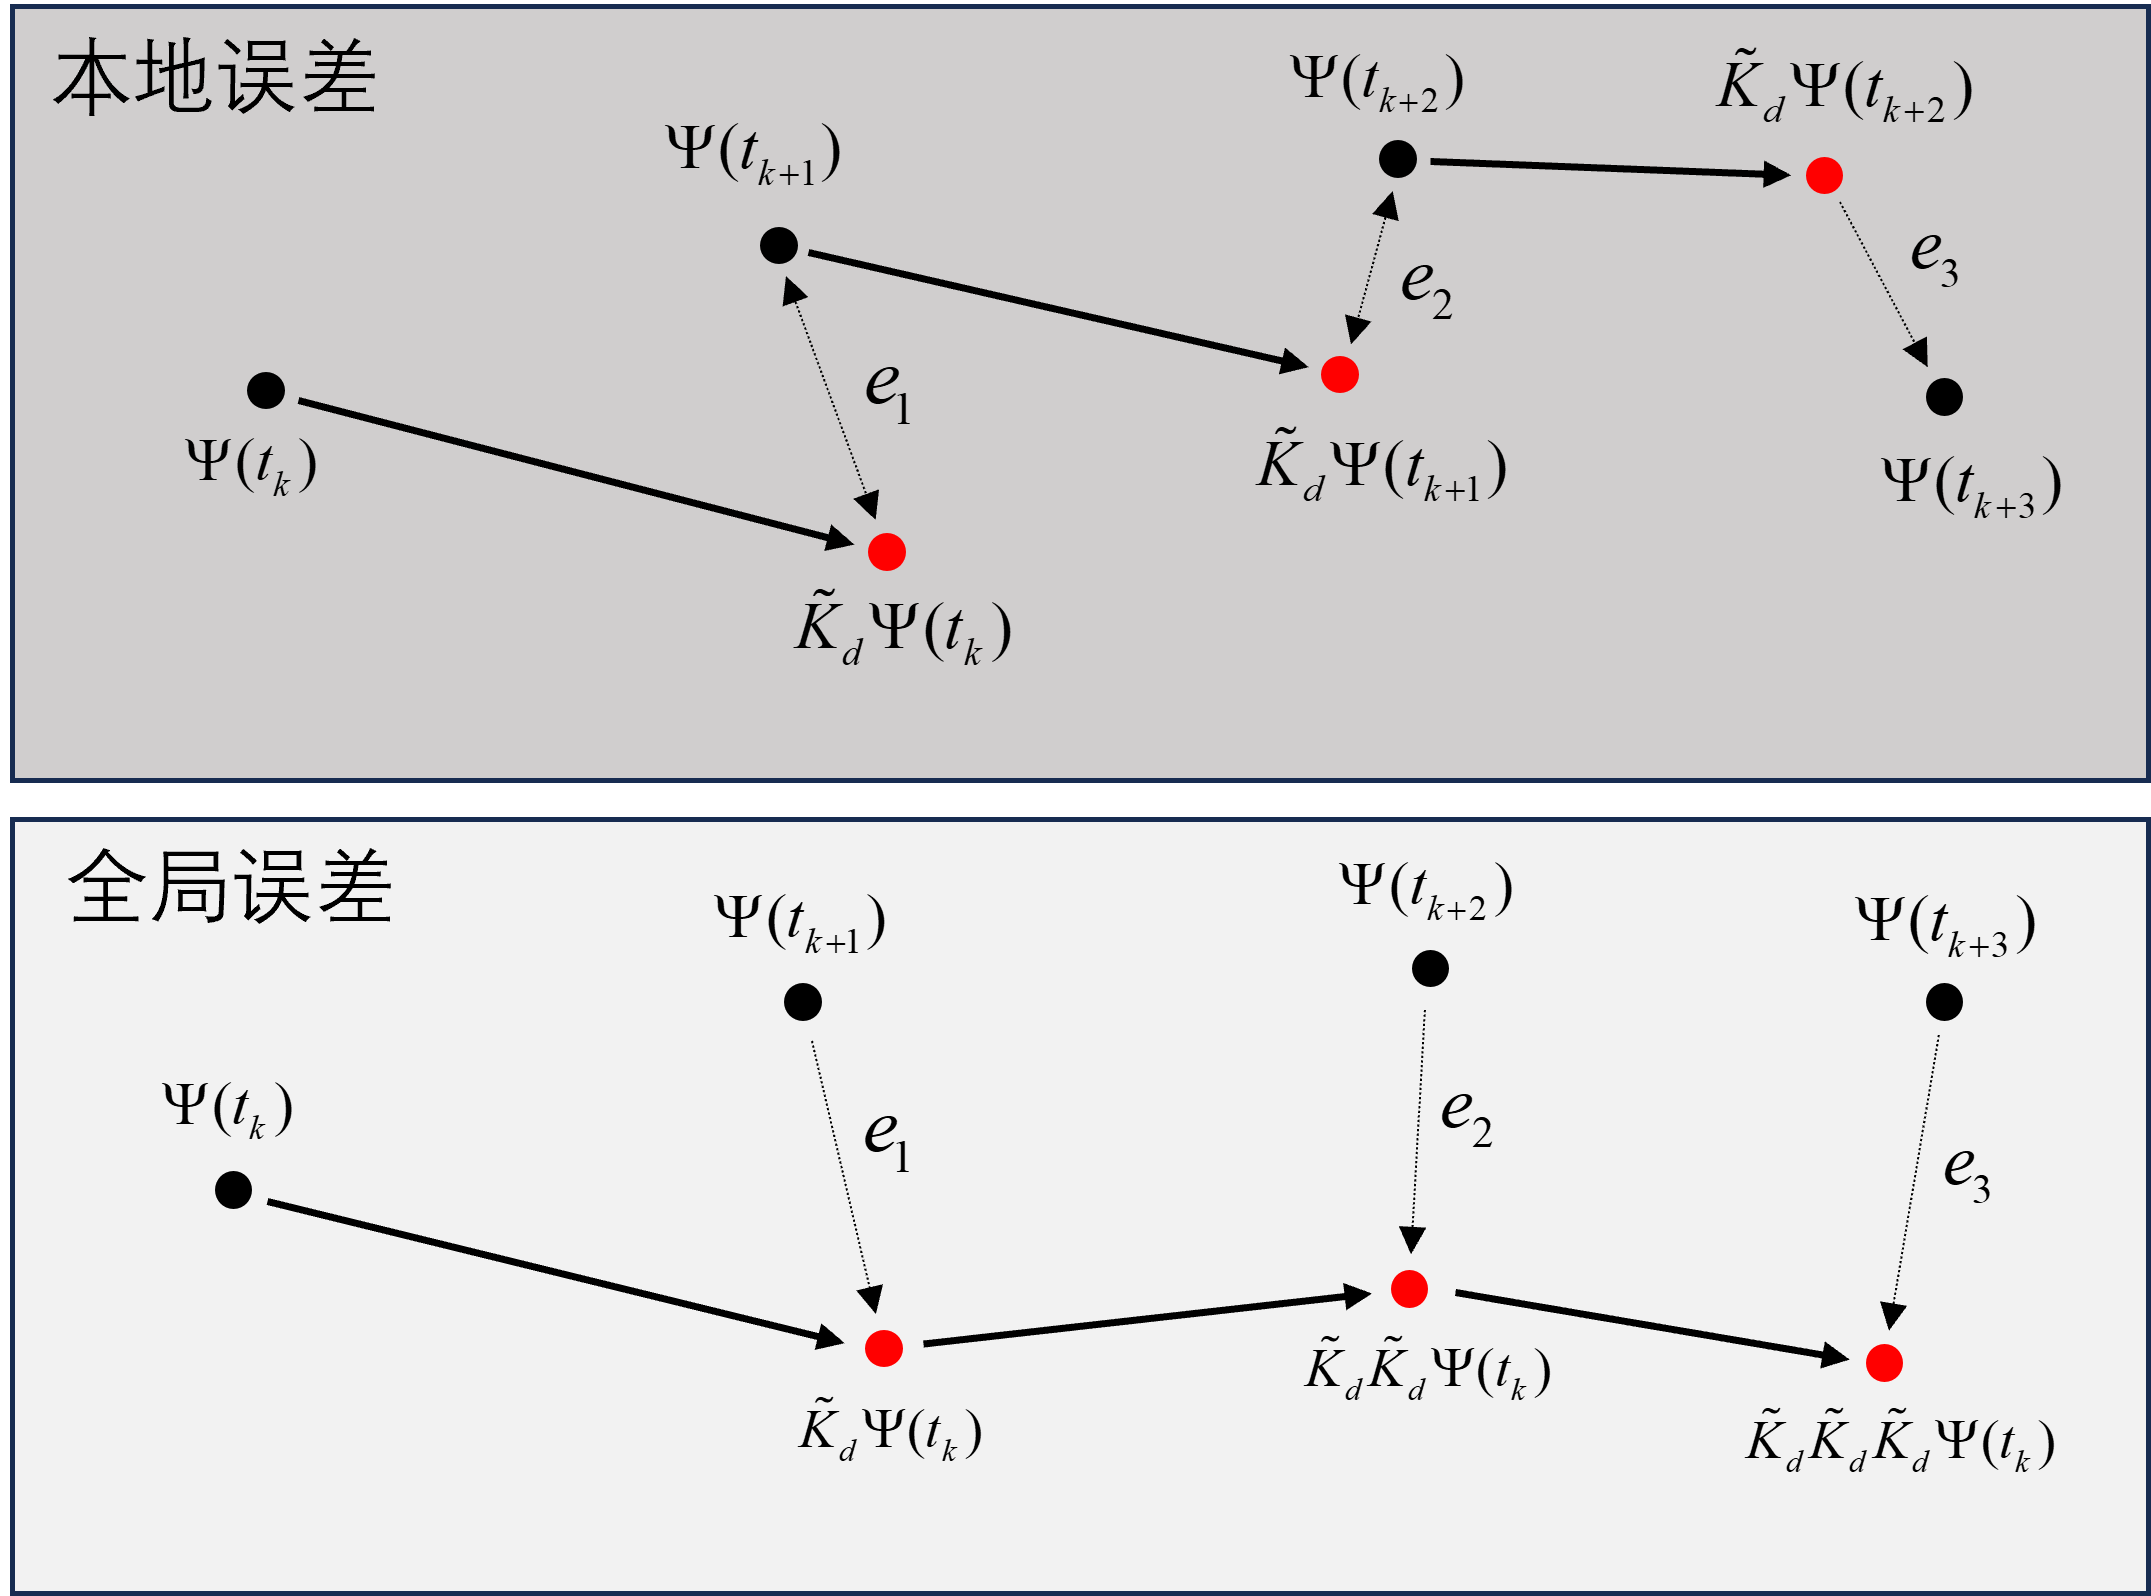
\includegraphics[width=30pc]{picture/3_2.png} 
	\caption{近似Koopman算子引起的局部误差和全局误差} \label{3_2}
\end{figure}
\subsection{基函数的Lipschitz常数约束}

如定理 \ref{error_boundness} 所述,如果基函数 $\bm{\Phi}$ 具有Lipschitz常数时,则预测误差是有界的。为了实现这一目标,用谱归一化(Spectral Normalization, SN)方法来约束基函数 $\bm{\Phi}$ 的Lipschitz常数。

根据定义,函数 $\rho$ 的Lipschitz常数等于其梯度的最大谱范数,即 $\Vert \rho \Vert_{\text{Lip}} = \sup \sigma (\nabla \rho)$。因此,对于由深度神经网络(\ref{dnn})参数化的基函数 $\bm{\Phi}$,可以通过限制每一层的谱范数来限定其Lipschitz常数。

线性层 $g(\bm{x})=\bm{W}\bm{x}$ 的Lipschitz常数为 $\Vert g \Vert_{\text{Lip}} = \sup \sigma(\nabla(g))=\sup \sigma(\bm{W})=\sigma(\bm{W})$。因此,基函数$\bm{\Phi}$的Lipschitz常数可以计算为(利用不等式 $\Vert g_1 \circ g_2 \Vert_{\text{Lip}} \le \Vert g_1 \Vert_{\text{Lip}}\cdot \Vert g_2 \Vert_{\text{Lip}}$):

\[
\begin{aligned}
	\Vert \bm{\Phi}(\bm{\chi}) \Vert_{\text{Lip}} &\le \Vert g^{L+1} \Vert_{\text{Lip}} \cdot \Vert \phi_L \Vert_{\text{Lip}} \cdots \Vert \phi_1 \Vert_{\text{Lip}} \cdot \Vert g_1 \Vert_{\text{Lip}} \\
	&= \prod_{l=1}^{L+1}\sigma(\bm{W}^l)
\end{aligned}
\]
其中,ReLU激活函数的Lipschitz常数为1,即 $\Vert \phi_l \Vert_{\text{Lip}} = 1$。在训练过程中,对每一层的权重 $\bm{W}$ 进行谱归一化可以表示为:

\[
\hat{\bm{W}} = \bm{W} / \sigma(\bm{W}) \cdot \gamma ^{\frac{1}{L+1}}  \label{sn}
\]


\begin{lemma} \label{lemma_lip}
	通过对基函数应用谱归一化(\ref{sn})方法之后,基函数的Lipschitz常数将满足以下约束:
	\[
	\Vert \bm{\Phi}(\bm{\chi}) \Vert_{\text{Lip}}\le \gamma
	\]
	其中,$\gamma$ 是基函数的目标Lipschitz常数。
\end{lemma}

\begin{proof}
	对DNN的每一层应用谱归一化之后,基函数的Lipschitz常数满足
	\[
	\Vert \bm{\Phi}(\bm{\chi}) \Vert_{\text{Lip}} \le \prod_{l=1}^{L+1}\sigma(\hat{\bm{W}}^l) = \prod_{l=1}^{L+1}\gamma^{\frac{1}{L+1}}=\gamma
	\]
	因此,通过谱归一化可以有效约束基函数的Lipschitz常数。
\end{proof}

综上所述,在深度神经网络的训练过程中,引入谱归一化技术不仅能够确保网络的Lipschitz常数满足特定的约束,还能提高模型的稳定性和泛化能力。这种方法在实现对嵌入函数约束的同时,避免了直接优化Lipschitz常数所带来的计算复杂性,从而为动态系统的学习提供了更加稳健的理论支撑。


\subsection{基于数据驱动下的学习动力学的控制器实现}

传统的鲁棒模型预测控制方法虽然能够有效应对系统中的不确定性,但其实际应用往往受到严格假设条件的限制,难以完全满足实际工程需求。此外,模型预测控制的闭环性能在很大程度上依赖于其内部模型的准确性,模型误差可能导致控制效果的下降。

为了解决这些问题,引入数据驱动预测模型的方法,利用其强大的数据拟合能力捕捉系统中难以建模或缺失的动态特性,从而显著提升控制器的整体性能和鲁棒性。
对于四旋翼无人机系绳吊运系统来说,使用基于Koopman理论的升维线性系统,对未知有效载荷和残余动力学引起的外力进行建模,捕获得到未知外力和力矩并集成到模型预测控制框架中,系统的模型以及状态和输入约束被考虑在如下形式的优化问题中:
\begin{equation}
	\begin{aligned} \label{nmpc}
		&\operatorname*{minimize}_{\bm{\bar{u}}}& & \sum_{i=0}^{N-1}\left(\bm{\bar{x}}_i^T\bm{Q}\bm{\bar{x}}_i + \bm{\bar{u}}_i^T\bm{R}\bm{\bar{u}}_i\right) + \bm{\bar{x}}_N^T\bm{P}\bm{\bar{x}}_N  \\
		&\text{subject to}& & \begin{aligned}
			&\bm{\bar{x}}_{0} = \bm{x}_k, \quad \bm{\bar{x}}_{N} \in \mathcal{X}_f, \\
			&\bm{\bar{x}}_{i+1} = \bm{f}_{\text{nominal}}(\bm{\bar{x}}_i, \bm{\bar{u}}_i) + \bm{f}_{\text{learned}},
		\end{aligned} \\
		&&& \bm{\bar{x}}_i \in \mathcal{X}, \quad \bm{\bar{u}}_i \in \mathcal{U}, \quad \forall i = 0, \ldots, N-1
	\end{aligned}
\end{equation}
其中,$\bm{x}_k$表示四旋翼在时间$k$时刻的状态,$\bm{\bar{x}}_i$和$\bm{\bar{u}}_i$分别是时间$k$的预测状态和控制输入,$N$是预测时域。$\mathcal{X}$、$\mathcal{U}$和$\mathcal{X}_f$分别是状态、控制输入和终端状态的约束集。$\bm{Q}$和$\bm{R}$是状态和控制输入的权重矩阵,$\bm{P}$是终端状态的权重矩阵。$\bm{f}_{\text{nominal}}$是四旋翼无人机的名义动力学,而$\bm{f}_{\text{learned}}$是通过升维线性系统学习得到的动态特性。

该优化问题通过序列二次规划(SQP)求解,并在实时迭代(RTI)方案中使用高斯-牛顿海森近似来提高计算效率。这种方法将学习到的动态特性融合到传统的名义模型里,从而提高控制器的性能和鲁棒性,整个算法的框架如图\ref{illustration_framework}所示,

\begin{figure}[hbt!]
	\centering
	\includegraphics[width=38pc]{picture/3_3.png} 
	\caption{数据驱动下的非线性模型预测控制框架} \label{illustration_framework}
\end{figure}
\section{仿真验证}


\section{本章总结}




\cleardoublepage

\chapter{多无人机吊运控制}
\chaptermark{多无人机吊运控制}

\section{引言}
建立航天器间精确碰撞约束后,服务星极近距离消旋位姿轨迹的规划得以进行。本章根据消旋任务的特点,将其划分为不同的阶段,针对不同阶段的任务需求,基于引导优化的规划框架,结合第三章所提出的碰撞风险评估方法,给出了各阶段位姿轨迹的规划方法,并通过仿真算例验证了所提极近距离消旋位姿轨迹规划方法的有效性。

\section{任务流程分析}




\section{极近距离逼近段位姿轨迹规划}
\subsection{逼近阶段参考路径搜索}
航天器轨迹规划领域常用的随机搜索方法主要为快速拓展随机树法(RRT*)及其衍生算法如informed-RRT*、RRT-Connect等,具有概率完备、渐近最优等优良特性,但对于高维问题,RRT*算法存在计算负荷、耗时较大等问题。针对高维构型空间中的复杂运动规划问题,Janson等提出快速行进树算法(FMT*)\cite{jansonFastMarchingTree2015},与RRT*算法相比,FMT*保留了渐近最优等特性,同时显著提升了收敛速度,具有较大的应用潜力。

基于FMT*算法的基本框架,本文所使用的针对航天器极近距离逼近问题的改进FMT*算法伪代码如表\ref{FMT}所示,主要分为初始化、节点搜索、反向链接、行进树拓展、节点更新等步骤。

%\renewcommand{\algorithmcfname}{算法4 -}
%\renewcommand{\algorithmicfname}{\textbf{算法4}}
\begin{algorithm}[htb]  
	\caption{FMT*搜索算法}  
	\label{FMT}  
	\begin{algorithmic}[1]  
		\Require  
		初始点$\boldsymbol{q}_{init}$,
		目标点$\boldsymbol{q}_{goal}$,
		样本点集$\mathbb{Q}_{sample}$
		\Ensure  
		从$\boldsymbol{q}_{init}$到$\boldsymbol{q}_{goal}$的最优位姿路径$\Gamma_{P}$
		\State $\operatorname{AddToTree}\left(\Lambda,\boldsymbol{q}_{init}\right)$
		\State$\mathbb{Q}=\boldsymbol{q}_{init}\cup \boldsymbol{q}_{goal}\cup \mathbb{Q}_{sample}$
		\State $\mathbb{Q}_{unvisited}=\mathbb{Q} \backslash \boldsymbol{q}_{init}$
		\State $\mathbb{Q}_{active}=\boldsymbol{q}_{init}$
		\State $\mathbb{Q}_{finished}=\emptyset$ 
		\State $\boldsymbol{q}_{serach}$=$\boldsymbol{q}_{init}$
		\State $\mathbb{Q}_{child} = \operatorname{Near}\left(\mathbb{Q}_{unvisited}, \boldsymbol{q}_{serach}, r_n\right)$
		\While {$\boldsymbol{q}_{serach}\neq \boldsymbol{q}_{goal}$}
		\For {$\boldsymbol{q}_{child,i}\in \mathbb{Q}_{child}$}
		\State $\mathbb{Q}_{parent} = \operatorname{Near}\left(\mathbb{Q}_{active}, \boldsymbol{q}_{child,i}, r_n\right)$
		\State $\boldsymbol{q}_{parent,j_{\min}}=\arg \min \limits_{\boldsymbol{q}_{parent,j} \in \mathbb{Q}_{parent}}\{c(\boldsymbol{q}_{parent,j})+\operatorname{Cost}\left(\boldsymbol{q}_{parent,j}, \boldsymbol{q}_{child,i}\right)\} \quad$
		\If {$\operatorname{CollisionFree}\left(\boldsymbol{q}_{parent,j_{\min}},\boldsymbol{q}_{child,i} \right)$}
		\State $\operatorname{AddToTree}\left(\Lambda,\boldsymbol{q}_{child,i}\right)$
		\State $\mathbb{Q}_{active}=\mathbb{Q}_{active}\cup \boldsymbol{q}_{child,i}$
		\State $\mathbb{Q}_{unvisited}=\mathbb{Q}_{unvisited}\backslash \boldsymbol{q}_{child,i}$
		\EndIf
		\EndFor
		\State $\mathbb{Q}_{finished}=\mathbb{Q}_{finished}\cup \boldsymbol{q}_{serach}$
		\If {$\mathbb{Q}_{active}=\empty$}
		\State \Return Failure
		\EndIf
		\State $\boldsymbol{q}_{serach}=\arg \min \limits_{\boldsymbol{q}_{sample} \in \mathbb{Q}_{active}}\{c(\boldsymbol{q}_{sample})\} \quad$
		\EndWhile
		\State $\Gamma_{P}=\operatorname{GetPath}\left(\Lambda \right)$
		\State \Return $\Gamma_{P}$
	\end{algorithmic}
\end{algorithm}

由于需对位姿进行同步规划,为便于遍历,采用欧拉角来描述章动目标和追踪星间的相对姿态,故样本点$\boldsymbol{q}=[{\boldsymbol{x}}_{\mathcal{B}}^{\mathcal{L}};\boldsymbol{\varphi}_{\mathcal{B}}^{\mathcal{L}}]$,其中$\boldsymbol{\varphi}_{\mathcal{B}}^{\mathcal{L}}$为$\mathcal{B}$系到$\mathcal{L}$系的欧拉角。

在初始化阶段,与RRT*算法在搜索过程中生成样本点不同,FMT*算法需使用预先生成的样本点,为保证样本点能充分遍历状态空间,本文采用霍尔顿序列(Halton sequence)生成样本点。霍尔顿序列是一种常用的低差异序列,任意一个质数都可以作为基底生成一组霍尔顿序列,其原理是根据所选基底对区间进行逐次分割,通过这种方式获得的伪随机数分布较为均匀,如图\ref{fig-halton}所示。

\begin{figure}[htbp]
	\centering
	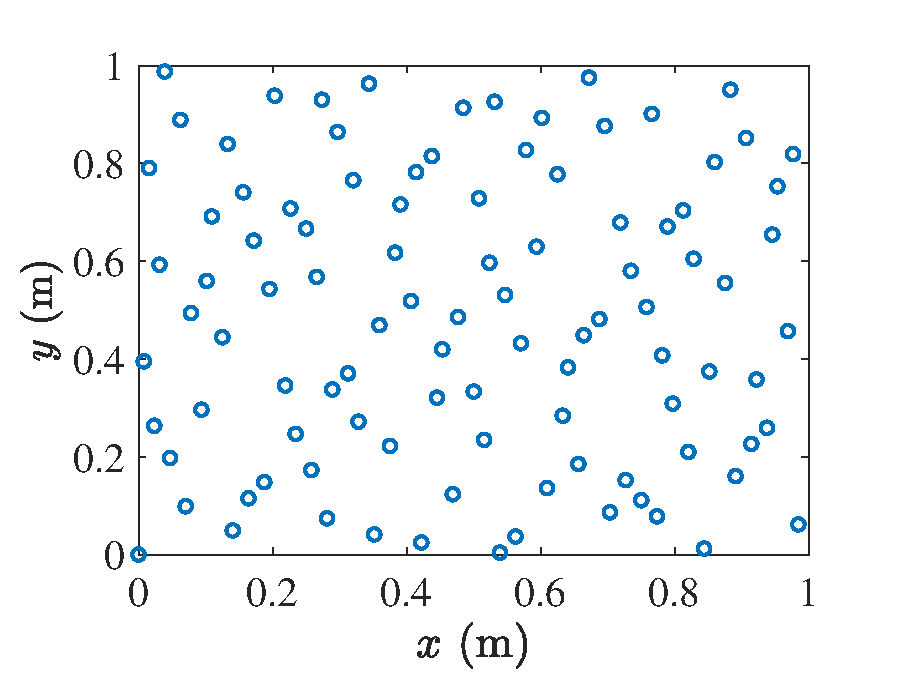
\includegraphics[width=2.8 in]{picture/haltonset.eps}
	\caption{二维霍尔顿序列示意图}
	\label{fig-halton}
\end{figure}

随后,通过\autoref{eq76}判别各样本点的可行性,删去不可行的样本点,把剩余的样本点和起始点、目标点输入FMT*算法中。建立$\mathbb{Q}_{unvisited}$,$\mathbb{Q}_{active}$和$\mathbb{Q}_{finished}$三个集合,将起始点$\boldsymbol{q}_{init}$添加至集合$\mathbb{Q}_{active}$中,其余节点添加至集合$\mathbb{Q}_{unvisited}$中。

节点间代价定义为:
\begin{equation}
	cost(\boldsymbol{q}_{i}-\boldsymbol{q}_{j}) =\Vert {\boldsymbol{x}}_{\mathcal{B},i}^{\mathcal{L}}-{\boldsymbol{x}}_{\mathcal{B},j}^{\mathcal{L}}\Vert_2+K_{\varphi}\Vert \boldsymbol{\varphi}_{\mathcal{B},i}^{\mathcal{L}}-\boldsymbol{\varphi}_{\mathcal{B},j}^{\mathcal{L}}\Vert_2
\end{equation}

采用Kd树结构存储节点信息,称$cost(\boldsymbol{q}_{i}-\boldsymbol{q}_{j})<r_{n}$的两节点为相邻节点,算法示意图如图\ref{Fig.fmt}所示。首先记$\mathbb{Q}_{active}$中到达代价最小的点为当前搜索节点$\boldsymbol{q}_{serach}$,通过Near函数将$\boldsymbol{q}_{serach}$的相邻节点中位于$\mathbb{Q}_{unvisited}$的节点记为待选子节点$\boldsymbol{q}_{child,i}$。

\begin{figure*}[htb!]
	\centering
	\begin{minipage}[t]{0.96\textwidth}
		\begin{subfigure}[t]{0.47\textwidth}
			\centering
			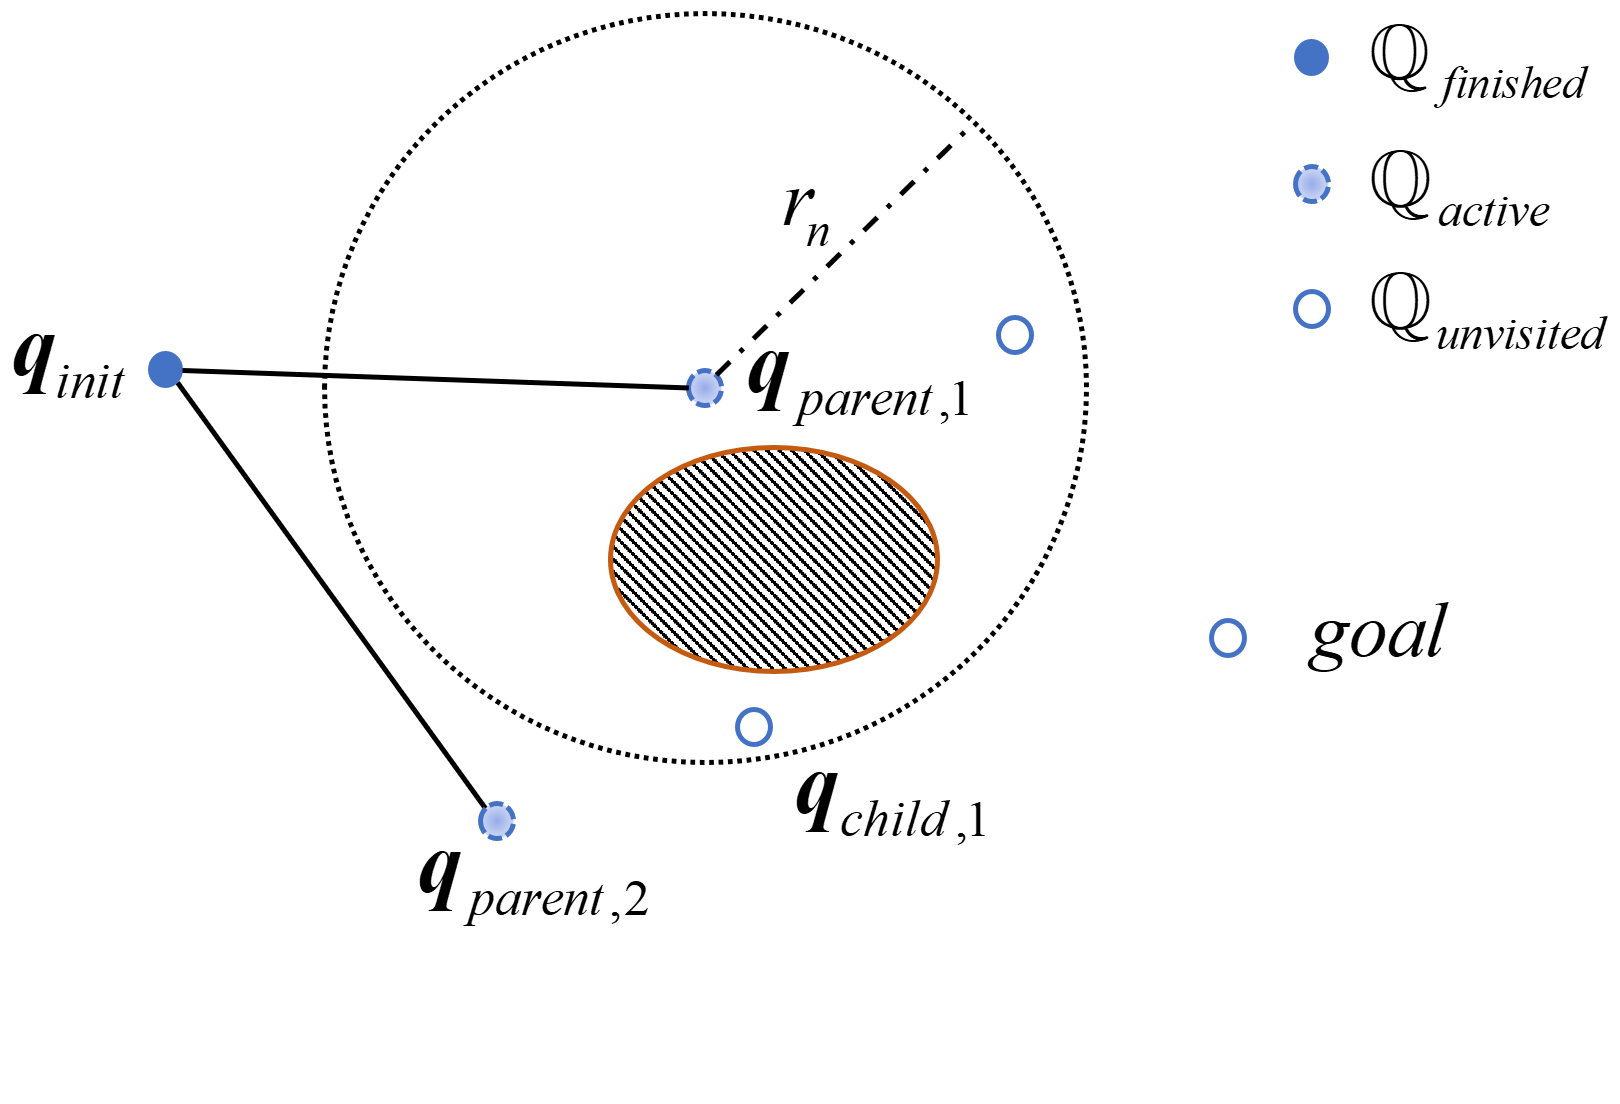
\includegraphics[width = 2.5in]{picture/FMT1.png}
			\caption{ }
			\label{fig:FMT(1)}
		\end{subfigure}\hfill
		\begin{subfigure}[t]{0.47\textwidth}
			\centering
			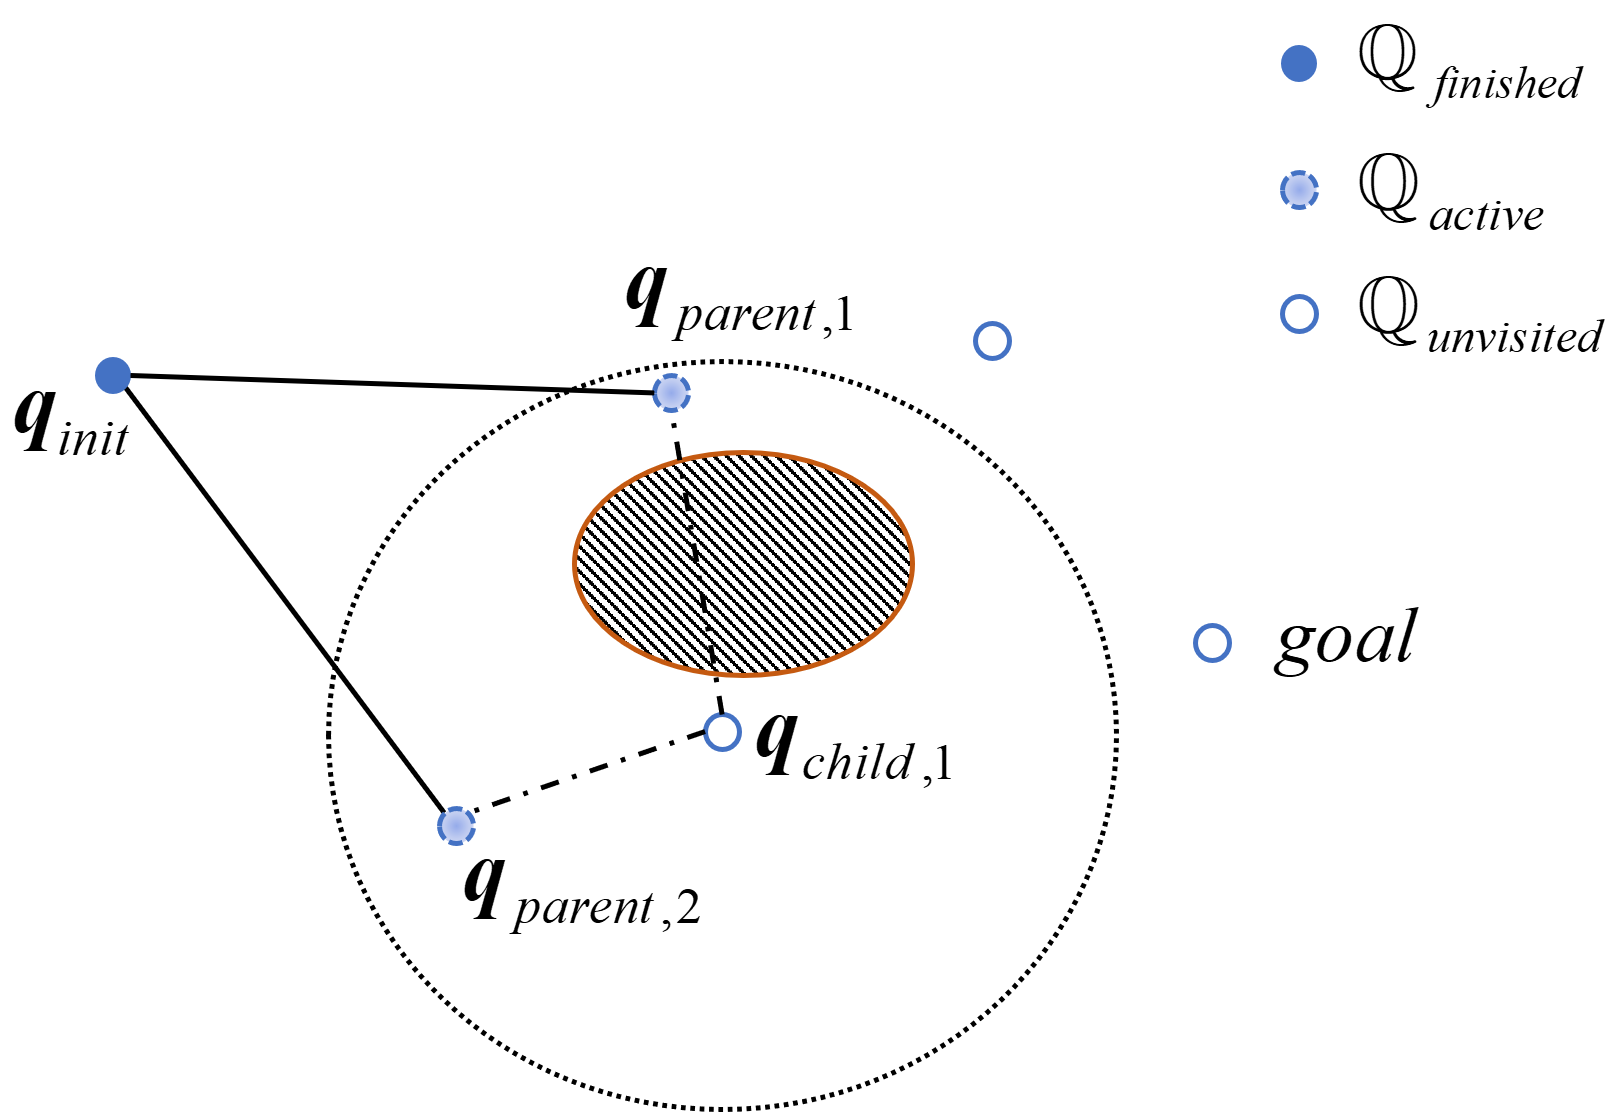
\includegraphics[width = 2.5in]{picture/FMT2.png}
			\caption{ }
			\label{fig:FMT(2)}
		\end{subfigure}
		
		\vspace{10pt}
		\begin{subfigure}[t]{0.47\textwidth}
			\centering
			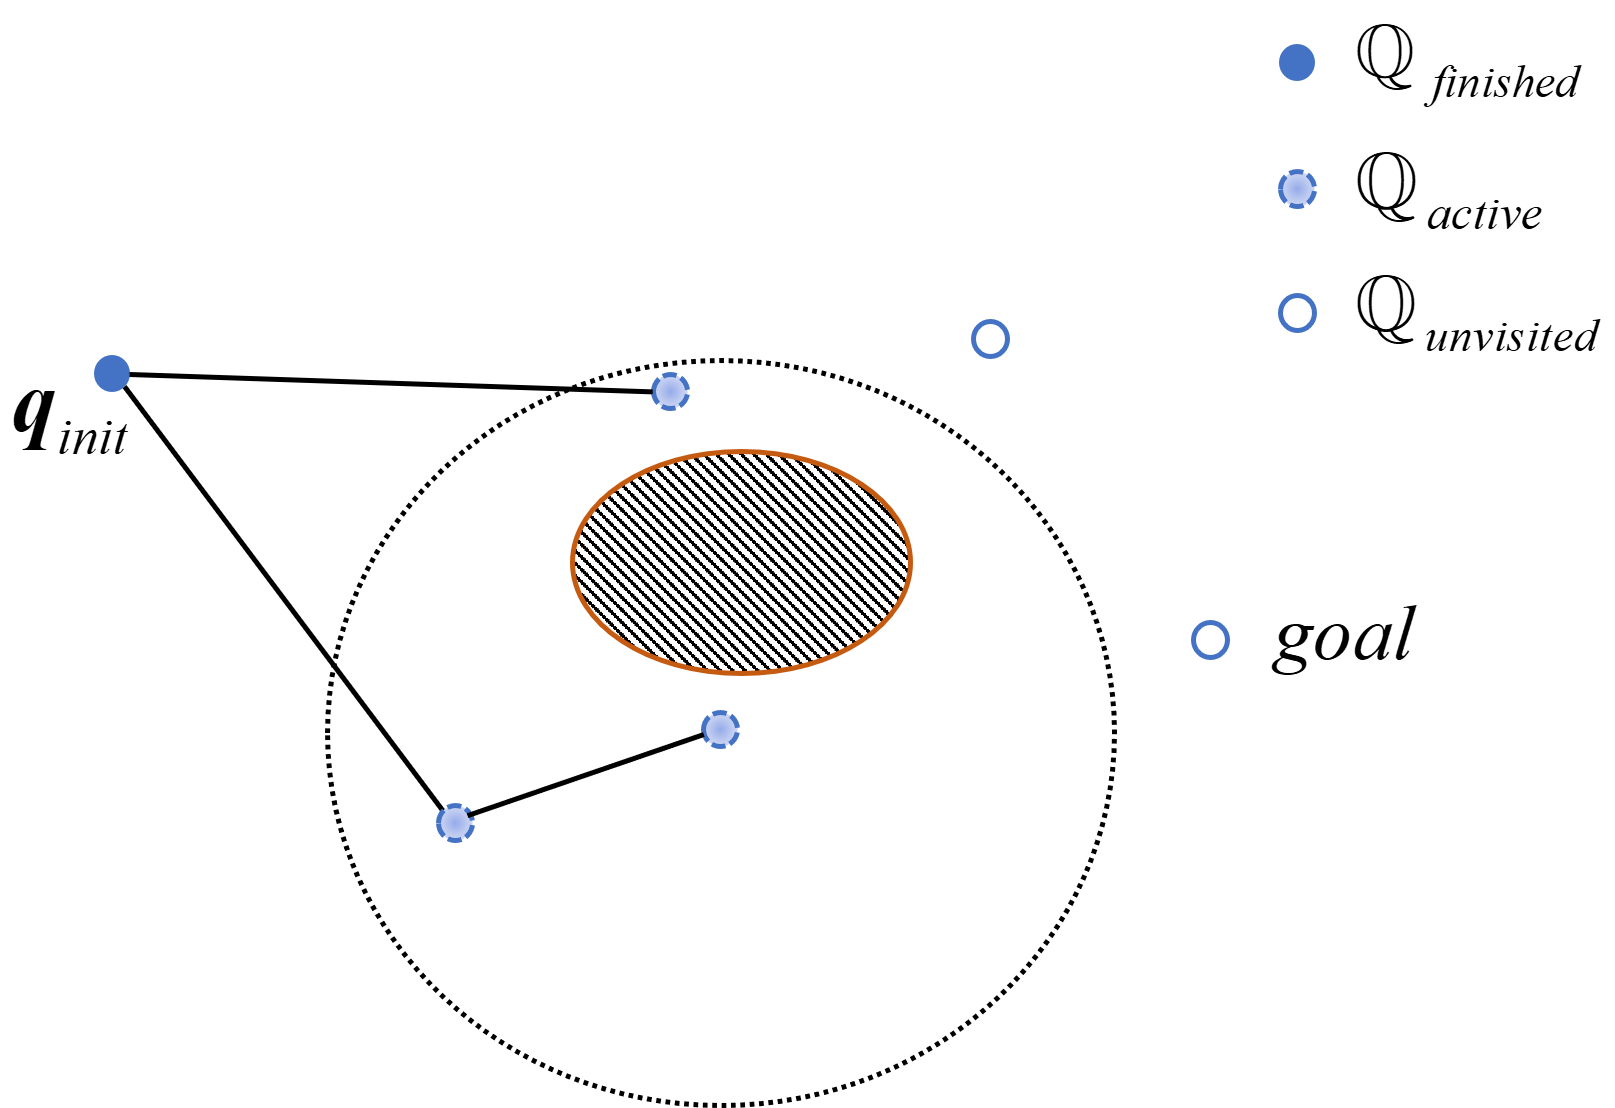
\includegraphics[width = 2.5in]{picture/FMT3.png}
			\caption{ }
			\label{fig:FMT(3)}
		\end{subfigure}\hfill
		\begin{subfigure}[t]{0.47\textwidth}
			\centering
			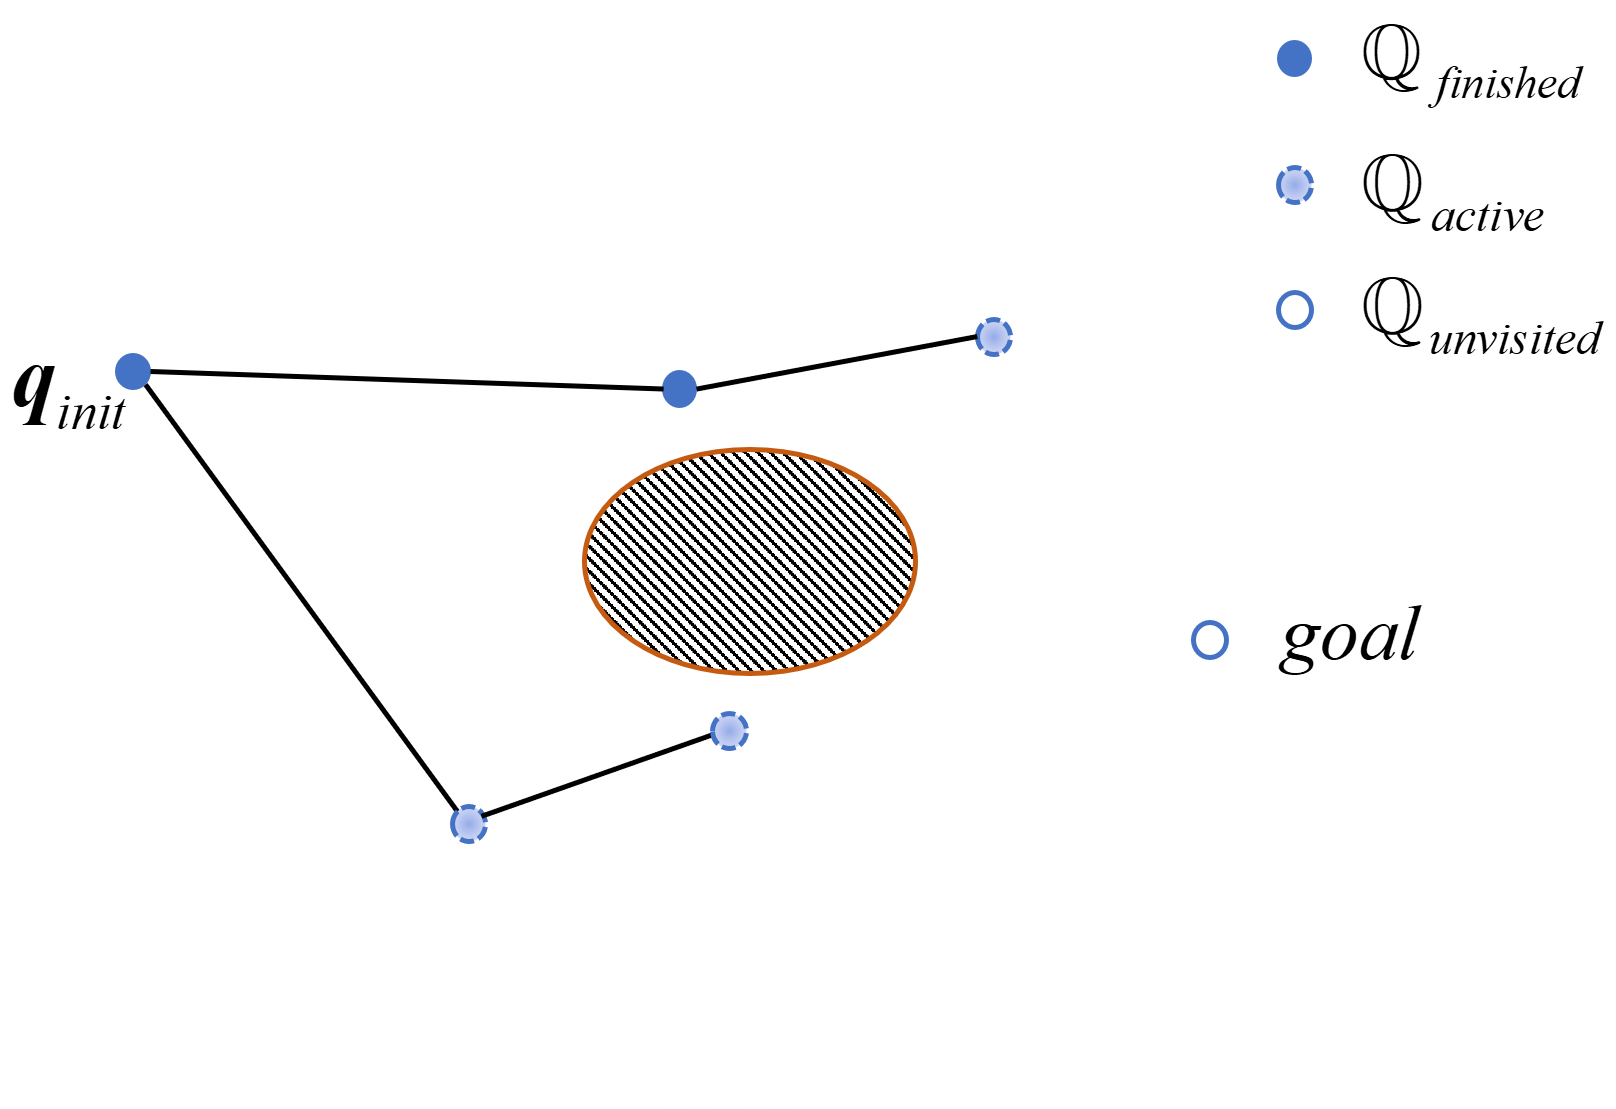
\includegraphics[width = 2.5in]{picture/FMT4.png}
			\caption{ }
			\label{fig:FMT(4)}
		\end{subfigure}
	\end{minipage}
	\caption{快速行进树算法示意图\label{Fig.fmt}}
\end{figure*}

接着在反向链接阶段,对各待选子节点进行遍历,在$\mathbb{Q}_{active}$中搜索$\boldsymbol{q}_{child,i}$的相邻节点,将其记为待选父节点$\boldsymbol{q}_{parent,j}$并确定代价最小的$\boldsymbol{q}_{parent,j_{\min}}$。

随后,CollisionFree函数将在$\boldsymbol{q}_{parent,j_{\min}}$和$\boldsymbol{q}_{child,i}$间均匀取点,判断二者连线是否无碰撞。若无碰撞,将$\boldsymbol{q}_{child,i}$加入行进树中,其父节点记为$\boldsymbol{q}_{parent,j_{\min}}$,完成行进树拓展,否则将跳转至下一个待选子节点。

所有待选子节点遍历完成后,对节点状态进行更新,将添加到行进树中的$\boldsymbol{q}_{child,i}$从$\mathbb{Q}_{unvisited}$中移除并添加至$\mathbb{Q}_{active}$中,将$\boldsymbol{q}_{serach}$加入$\mathbb{Q}_{finished}$中。到达目标点或$\mathbb{Q}_{active}$中无节点后算法结束,得到逼近阶段服务星参考路径。

从上述过程中不难看出,FMT*算法采用了惰性的拓展策略,只有当前最优路径可行时才把节点加入树中,否则就跳过该节点继续搜索其他节点,直到后续遍历过程中找到该节点的最优路径。这种策略省去了RRT*算法中的父节点重选步骤,且添加新节点时仅需进行一次碰撞检测,大大降低了碰撞检测的次数,因此在处理高维复杂问题时FMT*算法具有更好的表现\cite{jansonFastMarchingTree2015},与本文中约束复杂、位姿耦合的规划问题匹配度较好,可以给出一条无碰撞的距离最优参考轨迹。

\subsection{逼近阶段轨迹优化}
上述改进FMT*算法给出了逼近阶段的参考路径$\Gamma_{P}$,但该路径在各节点处不光滑,且未对速度、加速度进行约束,因此需要对其进行优化。本章采用B样条曲线构造光滑轨迹,并对其控制点参数进行优化,使其轨迹安全可行。

如前所述,B样条曲线的参数包括控制点集$\mathbb{C}=\{\boldsymbol{C}_{i}|i=1,2,\cdots,N_c\}$,节点向量$\boldsymbol{t}_{c}=[t_1,t_2,\cdots,t_{M_{t}}]$与曲线阶数$k_{o}$等。本文以控制点集\footnote{为保证轨迹经过给定的起始点与终点,取控制点集中的${c}_{1},{c}_{2}$和${c}_{N_c-1},{c}_{N_c}$为参考路径上的对应点,不进行优化}及节点向量为优化变量,将逼近阶段轨迹优化分为两个部分,第一部分的优化目标是在保证轨迹平滑度的前提下尽可能接近上一节给出的参考逼近路径$\Gamma_{P}$;第二部分的优化目标是进一步保证轨迹安全可行,同时对最小化所需的性能指标。考虑到优化变量数量较多,约束较为复杂,为保证问题求解的成功率与效率,两部分都采取软约束的方式将约束作为罚函数放入代价函数中,优化问题可表示为:
\begin{equation}
	\label{tra_cost_func}
	\mathop{\arg\min}\limits_{\mathbb{C},\boldsymbol{t}_{c}} \sum_{j=1}^{L_c} \pi_{j}f_{j}(\mathbb{C},\boldsymbol{t}_{c})
\end{equation}
其中$L_c$为待优化的指标数量,$f_{j}$为优化指标,$\pi_{j}$为权重值。

第一部分的优化指标包括轨迹平滑度$f_{s}$和路径相似度指标$f_{d}$,此部分不涉及节点向量的优化,故通过控制点间的几何关系来衡量轨迹平滑度$f_{s}$\cite{zhijiezhuConvexOptimizationApproach2015}:
\begin{equation}
	\label{smooth}
	f_{s}=\sum_{i=k_{o}-1}^{N_{c1}-k_{o}+1}\Vert\boldsymbol{C}_{i+1}-2 \boldsymbol{C}_i+\boldsymbol{C}_{i-1}\Vert_2
\end{equation}
该指标将使控制点尽可能处在前后控制点的连线上,减少不必要的波动以提升轨迹的平滑度。

同时,根据控制点的数量,在参考逼近路径$\Gamma_{P}$上均匀取点作为参考点$\boldsymbol{G}_{P,i}(i=1,2,\cdots,N_{c1})$,定义路径相似度$f_{d}$为:
\begin{equation}
	f_{d}=\sum_{i=k_{o}-2}^{N_{c1}-k_{o}+2}\Vert \boldsymbol{C}_i-\boldsymbol{G}_{P,i}\Vert_2
\end{equation}

故由\autoref{tra_cost_func},第一部分的优化问题可表示为:
\begin{equation}
	\begin{aligned}
		\label{proximity_phase1}
		\mathop{\arg\min}\limits_{\mathbb{C}} f_{P1}=&\pi_{s}f_{s}+\pi_{d}f_{d}\\
		=&\pi_{s}\sum_{i=k_{o}-1}^{N_{c1}-k_{o}+1}\Vert\boldsymbol{C}_{i+1}-2 \boldsymbol{C}_i+\boldsymbol{C}_{i-1}\Vert_2+\pi_{d}\sum_{i=k_{o}-2}^{N_{c1}-k_{o}+2}\Vert \boldsymbol{C}_i-\boldsymbol{G}_{P,i}\Vert_2
	\end{aligned}
\end{equation}

从上式中不难看出,该优化问题为无约束二次规划问题,其最优解具有解析表达式,将其解记为$\mathbb{C}_{Pw}$,代入\autoref{Bspline}中可得一条在参考路径附近的平滑轨迹$\mathbb{T}_{Pw}$。该轨迹无法保证各部分均无碰撞,且未对各项性能指标进行优化,因此不能作为最终轨迹。但由于参考路径是无碰撞的,$\mathbb{T}_{Pw}$的主体部分也是无碰撞的,可将$\mathbb{C}_{Pw}$作为下一部分优化的初值以降低下一部分优化失败的概率\cite{zhouRobustRealtimeUAV2020}。

逼近阶段轨迹优化第二部分的目标是保证轨迹安全可行,并减少轨迹的耗时与控制消耗,优化变量为控制点集$\mathbb{C}$及节点向量$\boldsymbol{t}_{c}$,优化指标包括轨迹平滑度$f_{s}$、碰撞惩罚$f_{c}$、速度及角速度平滑度$f_{vs}$、速度及加速度可行度$f_{f}$、耗时$f_{t}$等。同时,为保证轨迹起点和终点速度可为$\boldsymbol{0}$,本部分的首末控制点具有二阶重复度,即控制点数量$N_c=N_{c1}+2$。

各项优化指标中,碰撞惩罚项根据上一章定义的碰撞危险度及其阈值计算。常见的障碍势函数仅能将轨迹推离障碍物,避障效果与权重值直接相关,难以确定合适的权重值保证轨迹不与障碍物碰撞。而本文中碰撞危险度阈值$P_{ts}$可由\autoref{eq72}计算,故将其引入碰撞惩罚项中,定义碰撞惩罚项$f_{c}$为:
\begin{equation}
	\label{collision_cost}
	f_{c}=\sum_{i=k_{o}-2}^{N_c-k_{o}+2}\left(\frac{\pi_{sc} P_c({\boldsymbol{x}}_{i},\boldsymbol{\varphi}_{i})}{P_{ts}(\boldsymbol{\varphi}_{i})}\right)^2
\end{equation}
其中,$\pi_{sc}$为安全裕度系数,通常为略大于$1$的常数。

由第三章仿真部分可知,碰撞危险度为距离的指数函数,两航天器距离较远时碰撞危险度极小,因而轨迹保守性较小,参数鲁棒性高,以满足极近距离操作任务的需求。当两航天器安全区域接近时,碰撞危险度将迅速增大,以碰撞危险度阈值为分母,当控制点处的碰撞危险度接近碰撞危险度阈值时,$f_{c}$将以指数级增大,变化量远高于其他指标,能有效保证轨迹的安全性。若考虑测量误差、控制偏差等因素需增大轨迹保守性时,可采用碰撞危险度全局极小值或增大$\pi_{sc}$的数量级,以增加航天器间的安全裕度。

为减小服务星的燃料消耗,应尽可能降低逼近轨迹中速度及角速度的变化量。B样条曲线各点处的速度与速度控制点$\boldsymbol{V}_i$和节点向量$\boldsymbol{t}_{c}$有关,仿照轨迹平滑度的定义,本文定义速度平滑度代价$f_{vs}$为:
\begin{equation}
	f_{vs}=\sum_{i=2}^{N_c-2}(\Vert\boldsymbol{v}_{i+1}-2 \boldsymbol{v}_i+\boldsymbol{v}_{i-1}\Vert_2+\Vert\boldsymbol{\omega}_{i+1}-2 \boldsymbol{\omega}_i+\boldsymbol{\omega}_{i-1}\Vert_2)+\pi_{ts}\sum_{i=pb+1}^{N_c}(\Vert t_{i+1}-2 t_i+t_{i-1}\Vert_2)
\end{equation}

如前所述,该指标将使速度控制点尽可能处于前后控制点的连线上,而B样条曲线具有凸包性,故该指标可减少轨迹的速度变化量,同时,节点向量间隔变化平缓能保证各轨迹点速度变化平缓,提升轨迹的速度平滑度。

考虑到服务星能提供的推力有限,为保证轨迹可行,需对轨迹的速度和加速度进行限制。设速度、角速度及对应的加速度限制分别为:$v_{\max}$,$\omega_{\max}$,$a_{\max}$,$\dot{\omega}_{\max}$,定义速度及加速度可行度$f_{f}$为:
\begin{equation}
	f_{f}=\sum_{i=1}^{N_c-1}\left(\left(\frac{\Vert\boldsymbol{v}_{i}\Vert_2}{v_{\max}}\right)^{2}+\left(\frac{\Vert\boldsymbol{\omega}_{i}\Vert_2}{\omega_{\max}}\right)^{2}\right)+\sum_{i=1}^{N_c-2}\left(\left(\frac{\Vert\boldsymbol{a}_{i}\Vert_2}{a_{\max}}\right)^{2}+\left(\frac{\Vert\boldsymbol{\dot{\omega}}_{i}\Vert_2}{\dot{\omega}_{\max}}\right)^{2}\right)
\end{equation}

此外,为避免对速度平滑度进行优化时无限制的增大节点向量,增加耗时指标$f_{t}$以保证轨迹耗时合理:
\begin{equation}
	f_{t}=t_{M_{t}}-t_{1}.
\end{equation}

综上所述,第二部分的轨迹优化问题可表示为:
\begin{equation}
	\begin{aligned}
		\label{proximity_phase2}
		\mathop{\arg\min}\limits_{\mathbb{C},\boldsymbol{t}_{c}} f_{P2}=&\pi_{s}f_{s}+\pi_{c}f_{c}+\pi_{vs}f_{vs}+\pi_{f}f_{f}+\pi_{t}f_{t}
	\end{aligned}
\end{equation}

将$\mathbb{C}_{Pw}$作为\autoref{proximity_phase2}中优化问题的初值进行求解,获得优化后的控制点集$\mathbb{C}_{Pf}$与节点向量$\boldsymbol{t}_{Pf}$,代入\autoref{Bspline}中,可得满足各项指标的服务星逼近位姿轨迹$\mathbb{T}_{Pf}$。

\section{极近距离消旋位姿轨迹规划}
当服务星完成极近距离逼近,开始对章动目标消旋后,目标的状态会逐渐发生变化,服务星当前位姿已不再是最佳消旋位姿,甚至可能与章动目标发生碰撞,因此需先求解新的最优消旋位姿,再给出一条安全的消旋轨迹。本文中认为目标章动角变化超过$1\ (^{\circ})$时需要对最优消旋位姿进行更新并机动至新的最优消旋位姿,由于服务星此时在对章动目标进行极近距离操作,最优消旋位姿和消旋轨迹的求解都需在给定时限内完成。

由于目标全运动周期型安全区域具有对称性,最优消旋位姿可能具有多组解,为减少不必要的机动,同时加快求解速度,将最优消旋位姿求解问题改为以下形式:
\begin{equation}
	\begin{aligned}
		\mathop{\arg\min}\limits_{{\boldsymbol{x}_{\mathcal{B}}^{\mathcal{L}}},{\boldsymbol{\varphi}_{\mathcal{B}}^{\mathcal{L}}}} &-\pi_{tor}\left(\Vert \boldsymbol{T}^{\mathcal{L}}_{Bt}\Vert_2 \right)+\pi_{tord}\left(\Vert \boldsymbol{T}^{\mathcal{L}}_{Bt} \times {\boldsymbol{\hat l}}_x \Vert_2\right)+\\
		&\pi_{dis}\left(\Vert {\boldsymbol{x}_{\mathcal{B}}^{\mathcal{L}}}-\boldsymbol{x}_{prev} \Vert_2+\Vert {\boldsymbol{\varphi}_{\mathcal{B}}^{\mathcal{L}}}-\boldsymbol{\varphi}_{prev} \Vert_2\right)+\pi_{col}\left(\frac{\pi_{sc} P_c({\boldsymbol{x}_{\mathcal{B}}^{\mathcal{L}}},{\boldsymbol{\varphi}_{\mathcal{B}}^{\mathcal{L}}})}{P_{ts,\min}}\right)^2
	\end{aligned}
\end{equation}
其中$\boldsymbol{x}_{prev}$和$\boldsymbol{\varphi}_{prev}$为服务星当前的相对位置和姿态。

求解上述问题获得新的最优消旋位姿后,就可以开始消旋轨迹的求解。多数时刻消旋位姿的变化不大,但当目标的章动角与初始时刻相比变化较大时,服务星可能需要进行机动以切换消旋构型,即本文采用切换构型的消旋策略,采用直线轨迹连接前后消旋位姿无法满足要求,需设计相应的轨迹规划方法。本文中消旋阶段服务星位姿轨迹的规划仍采用引导优化的框架,与上一阶段一致,但相比最优性此阶段更加强调规划的实时性,对轨迹的性能要求也有所不同,故本节对相关方法进行了修改以满足消旋阶段轨迹的要求。

\subsection{消旋阶段参考路径搜索}
为提高求解速度,消旋阶段的参考路径不再追求最优性,仅要求给出一条无碰撞的参考路径,故本文给出一种简单的路径生成算法PPO,其伪代码如表\ref{pull_out}所示。
\begin{algorithm}[htb]  
	\caption{Path Push Out算法(PPO)}  
	\label{pull_out}  
	\begin{algorithmic}[1]  
		\Require  
		初始点$\boldsymbol{q}_{init}$,
		目标点$\boldsymbol{q}_{goal}$,
		等分数$n_c$
		\Ensure  
		从$\boldsymbol{q}_{init}$到$\boldsymbol{q}_{goal}$的安全位姿路径$\Gamma_{D}$
		\State $\mathbb{Q}_{ori}=\operatorname{LinePoint}(\boldsymbol{q}_{init},\boldsymbol{q}_{goal},n_c)$
		\State $\boldsymbol{q}_{prev}=\boldsymbol{q}_{init}$
		\State $\mathbb{Q}_{free}=\boldsymbol{q}_{init}$
		\State $\boldsymbol{d}_{dec}=\operatorname{DescendDir}(\mathbb{Q}_{ori})$
		\For {$\boldsymbol{q}_{ori,i}\in \mathbb{Q}_{ori}$}
		\State $\boldsymbol{q}_{free}=\operatorname{PushOut}(\boldsymbol{q}_{ori,i},\boldsymbol{d}_{dec})$
		\If {$\operatorname{CollisionFree}(\boldsymbol{q}_{prev},\boldsymbol{q}_{free})$}
		\State $\mathbb{Q}_{free}=\mathbb{Q}_{free}\cup \boldsymbol{q}_{free}$
		\State $\boldsymbol{q}_{prev}=\boldsymbol{q}_{free}$
		\Else
		\State $\mathbb{Q}_{SubLine}=\operatorname{LinePoint}(\boldsymbol{q}_{prev},\boldsymbol{q}_{free},n_c)$
		\State $\boldsymbol{d}_{Subdec}=\operatorname{DescendDir}(\mathbb{Q}_{SubLine})$
		\For {$\boldsymbol{q}_{SubLine,i}\in \mathbb{Q}_{SubLine}$}
		\State $\boldsymbol{q}_{free}=\operatorname{PushOut}(\boldsymbol{q}_{SubLine,i},\boldsymbol{d}_{Subdec})$
		\State $\mathbb{Q}_{free}=\mathbb{Q}_{free}\cup \boldsymbol{q}_{free}$
		\EndFor
		\State $\boldsymbol{q}_{prev}=\boldsymbol{q}_{free}$
		\EndIf
		\EndFor
		\State $\Gamma_{D}=\operatorname{LinePath}(\mathbb{Q}_{free})$
		\State \Return $\Gamma_{D}$
	\end{algorithmic}
\end{algorithm}

算法首先将初始点记为$\boldsymbol{q}_{prev}$,存入$\mathbb{Q}_{free}$中。通过LinePoint函数在起始点和目标点间进行线性插值,获取该直线路径上的等分点,并将这些点存入集合$\mathbb{Q}_{ori}$中。

随后通过DescendDir函数计算各路径点碰撞梯度确定搜索的方向。其中,路径点$\boldsymbol{q}$中的姿态项仅用于计算位置项的梯度$\boldsymbol{g}_{x}$,不对姿态项的梯度进行计算,梯度计算公式如\autoref{grad_p}所示。考虑到平行于路径方向的梯度分量仅会使路径点间隔被拉大,导致路径搜索失败,仅保留由\autoref{verti_grad}计算的垂直路径方向的梯度分量$\boldsymbol{g}_{xv}$。同时,为避免搜索后各路径点的分布过于分散,算法中各路径点采用相同的搜索方向$\boldsymbol{d}_{dec}$,该向量为各路径点梯度的加权求和,由\autoref{dec_vec}计算。

\begin{equation}
	\begin{aligned}
		\label{grad_p}
		\boldsymbol{g}_{x}=&\frac{\partial{P_c({\boldsymbol{x}}_{\mathcal{B}}^{\mathcal{L}},\boldsymbol{\varphi}_{\mathcal{B}}^{\mathcal{L}})}}{\partial{{\boldsymbol{x}}_{\mathcal{B}}^{\mathcal{L}}}}\\
		=&-\sum\limits_{f = 1}^F {\sum\limits_{j = 1}^J {{\pi _f}} } {\pi _j}N(\boldsymbol{x}_{\mathcal{B}}^{\mathcal{L}}|{{\boldsymbol{\mu }}_f} - {\boldsymbol{R}}_{\mathcal{B}}^{\mathcal{L}}{{\boldsymbol{\mu }}_j},{{\boldsymbol{\Sigma }}_f} + {\boldsymbol{R}}_{\mathcal{B}}^{\mathcal{L}}{{\boldsymbol{\Sigma }}_j}{({\boldsymbol{R}}_{\mathcal{B}}^{\mathcal{L}})^{\top}})\\
		&\left({{\boldsymbol{\Sigma }}_f} + {\boldsymbol{R}}_{\mathcal{B}}^{\mathcal{L}}{{\boldsymbol{\Sigma }}_j}{({\boldsymbol{R}}_{\mathcal{B}}^{\mathcal{L}})^{\top}}\right)^{-1}\left({\boldsymbol{x}}_{\mathcal{B}}^{\mathcal{L}}-{{\boldsymbol{\mu }}_f} + {\boldsymbol{R}}_{\mathcal{B}}^{\mathcal{L}}{{\boldsymbol{\mu }}_j}\right)
	\end{aligned}
\end{equation}

\begin{equation}
	\label{verti_grad}
	\boldsymbol{g}_{xv}=\boldsymbol{g}_{x}-(\boldsymbol{d}_{l}^{\top}\boldsymbol{g}_{x})\boldsymbol{d}_{l}
\end{equation}
其中,$\boldsymbol{d}_{l}$是由起始位置指向目标位置的单位向量。

\begin{equation}
	\label{dec_vec}
	\boldsymbol{d}_{dec}=\sum_{i=1}^{n_c} \pi_{g,i}\boldsymbol{g}_{xv,i}
\end{equation}
其中$\pi_{g,i}$为第$i$个路径点的权重,由下式计算:
\begin{equation}
	\pi_{g,i}= \log\left(\frac{P_c({\boldsymbol{x}}_i,\boldsymbol{\varphi}_i)}{P_{ts}(\boldsymbol{\varphi}_i)}\right)
\end{equation}

确定路径搜索方向后,调用PushOut函数对点集$\mathbb{Q}_{ori}$中的每个路径点进行检测。通过\autoref{eq76}进行碰撞判定,若该路径点无碰撞,则保持不变,否则沿$\boldsymbol{d}_{dec}$方向进行一维搜索,找到对应的无碰撞点,记为$\boldsymbol{q}_{free}$。若$\boldsymbol{q}_{free}$与$\boldsymbol{q}_{prev}$间无碰撞,将$\boldsymbol{q}_{free}$添加至$\mathbb{Q}_{free}$中,对$\boldsymbol{q}_{prev}$进行更新并进行下一次遍历;否则在$\boldsymbol{q}_{free}$与$\boldsymbol{q}_{prev}$间均匀取点,重复上述过程以给出$\boldsymbol{q}_{free}$与$\boldsymbol{q}_{prev}$间的无碰撞路径。遍历结束后,LinePath函数将连接$\mathbb{Q}_{free}$中的各路径点给出一条无碰撞位姿路径$\Gamma_{D}$,如图\ref{Fig.PPO}所示。

\begin{figure}[hbt!]
	\centering
	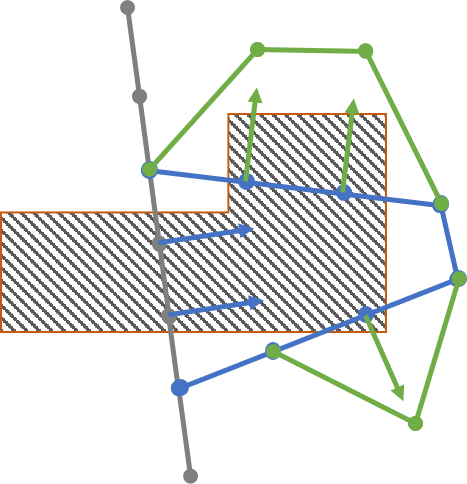
\includegraphics[width=2.5 in]{picture/PPO_pic.png}
	\caption{PPO算法示意图\label{Fig.PPO}}
\end{figure}

可以看出,当起始点与目标点相距较近,二者间连线无碰撞时,PPO算法将直接给出一条连接起始点和目标点的直线路径。当直线路径无法满足要求时,PPO对路径点中的姿态项仍进行直线插值,随后对位置项沿计算的梯度下降方向进行一维搜索,在至多$n_c^2$次遍历内给出一条参考路径,保证了算法收敛的快速性。

\subsection{消旋阶段轨迹优化}
与逼近阶段类似,获得无碰撞的参考消旋路径后,本节将采用基于B样条曲线的轨迹优化方法,依次求解两个优化问题给出一条满足要求的消旋轨迹。

消旋轨迹优化第一部分的优化目标是在保证轨迹平滑度的前提下尽可能接近给出的参考路径$\Gamma_{D}$,与逼近阶段一致,优化问题可表示为:
\begin{equation}
	\begin{aligned}
		\label{detumbing_phase1}
		\mathop{\arg\min}\limits_{\mathbb{C}} f_{D1}=&\pi_{s}f_{s}+\pi_{d}f_{d}\\
		=&\pi_{s}\sum_{i=k_{o}-1}^{N_{c1}-k_{o}+1}\Vert\boldsymbol{C}_{i+1}-2 \boldsymbol{C}_i+\boldsymbol{C}_{i-1}\Vert_2+\pi_{d}\sum_{i=k_{o}-2}^{N_{c1}-k_{o}+2}\Vert \boldsymbol{C}_i-\boldsymbol{G}_{D,i}\Vert_2
	\end{aligned}
\end{equation}
其中$\boldsymbol{G}_{D,i}$为参考消旋路径$\Gamma_{D}$上均匀选取的参考点。

求解\autoref{detumbing_phase1}可得与参考路径接近的控制点集,将其记为$\mathbb{C}_{Dw}$。

消旋轨迹优化第二部分的优化目标是保证轨迹安全,同时最大化所施加的消旋力矩。为加快求解速度,优化变量仅包括控制点集$\mathbb{C}$,不对节点向量进行优化,优化指标包括轨迹平滑度$f_{s}$、碰撞惩罚$f_{c}$、有效力矩$f_{tor}$。

其中,轨迹平滑度$f_{s}$仍由\autoref{smooth}计算,碰撞惩罚项$f_{c}$中的碰撞危险度阈值改为由\autoref{ptsmin}确定的全局阈值以提高求解速率:
\begin{equation}
	\label{collision_cost2}
	f_{c}=\sum_{i=k_{o}-2}^{N_c-k_{o}+2}\left(\frac{\pi_{sc} P_c({\boldsymbol{x}}_{i},\boldsymbol{\varphi}_{i})}{P_{ts,\min}}\right)^2
\end{equation}

有效力矩$f_{tor}$为各控制点处能产生的消旋力矩之和,可表示为:
\begin{equation}
	f_{tor}=\sum_{i=k_{o}}^{N_c-k_{o}+1} -\Vert \boldsymbol{T}^{\mathcal{L}}_{Bt,i} \Vert_2
\end{equation}
其中$\boldsymbol{T}^{\mathcal{L}}_{Bt,i}$为控制点$\boldsymbol{C}_{i}$处能产生的消旋力矩。

故消旋轨迹优化第二部分的优化问题可表示为:
\begin{equation}
	\begin{aligned}
		\label{detumbing_phase2}
		\mathop{\arg\min}\limits_{\mathbb{C}} f_{D2}=\pi_{s}f_{s}+\pi_{c}f_{c}+\pi_{tor}f_{tor}
	\end{aligned}
\end{equation}

将$\mathbb{C}_{Dw}$作为\autoref{detumbing_phase2}中优化变量的初值,对\autoref{detumbing_phase2}进行求解,可得优化后的控制点集$\mathbb{C}_{Df}$。但\autoref{detumbing_phase2}中未对节点向量进行优化,各控制点的速度、加速度可能不在限制范围内,因此需对轨迹时间进行重分配,适当增大不可行控制点对应的时间间隔以保证轨迹可行。

由\autoref{vec_cal}可知,若第$i$个控制点的速度由时间间隔$\Delta t_{v} =t_{i+k_{o}+1}-t_{i+1}$决定,将$\Delta t$调整为$\pi_{ve}$倍后,其速度$\boldsymbol{V}_{i}$将变为:
\begin{equation}
	\begin{aligned}
		\boldsymbol{V}_{i}^{\prime}=\frac{k_{o}\left(\boldsymbol{C}_{i+1}-\boldsymbol{C}_i\right)}{\pi_{ve}t_{i+k_{o}+1}-t_{i+1}}
		=\frac{\boldsymbol{V}_{i}}{\pi_{ve}}
	\end{aligned}
\end{equation}

故对于速度超限的控制点,取$\pi_{ve}=\frac{\vert \boldsymbol{V}_{i}\vert_2}{v_{max}}+t_{\delta}$,并将$\Delta t_{v}$增大为$\pi_{ve}$倍即可使其速度满足约束,其中$t_{\delta}$为一微小正值。

类似的,第$i$个控制点的加速度由时间间隔$\Delta t_{a} =t_{i+k_{o}+2}-t_{i+1}$决定,将$\Delta t$调整为$\pi_{ae}$倍后,其加速度$\boldsymbol{A}_{i}$将变为
\begin{equation}
	\begin{aligned}
		\boldsymbol{A}_{i}^{\prime}=\frac{\left(k_{o}-1\right)\left(\boldsymbol{V}_{i+1}^{\prime}-\boldsymbol{V}_i^{\prime}\right)}{\pi_{ae}(t_{i+k_{o}+1}-t_{i+2})}
		=\frac{\left(k_{o}-1\right)\left(\boldsymbol{V}_{i+1}-\boldsymbol{V}_i\right)}{(\pi_{ae})^2(t_{i+k_{o}+1}-t_{i+2})}
		=\frac{\boldsymbol{A}_{i}}{(\pi_{ae})^2}
	\end{aligned}
\end{equation}

则取$\pi_{ae}=\sqrt{\frac{\vert \boldsymbol{V}_{i}\vert_2}{v_{max}}}+t_{\delta}$并将时间间隔$\Delta t_{a}$增大为$\pi_{ae}$倍即可保证该控制点的加速度满足约束。

通过上述公式对一个控制点对应的时间间隔进行调整后,会对其前后的控制点也产生影响,本文参考\cite{zhouRobustEfficientQuadrotor2019}采用迭代法调整节点向量,以保证各控制点的速度、角速度、加速度以及角加速度均满足约束,如表\ref{retime}所示。

\begin{algorithm}[htb]  
	\caption{控制点时间重分配算法}
	\label{retime}  
	\begin{algorithmic}[1]  
		\Require  
		控制点集$\mathbb{C}$,
		节点向量$\boldsymbol{t}_{Do}$,
		速度及加速度限制$\boldsymbol{B}=[v_{\max},\omega_{\max},a_{\max},\dot{\omega}_{\max}]$
		\Ensure  
		调整后满足约束的节点向量$\boldsymbol{t}_{Df}$
		\State $[\mathbb{V},\mathbb{A}]=\operatorname{FindInfeasible}(\mathbb{C},\boldsymbol{t}_{Do},\boldsymbol{B})$
		\State $\boldsymbol{t}_{Df}=\boldsymbol{t}_{Do}$
		\While{$ !\operatorname{IsEmpty}(\mathbb{V},\mathbb{A})$}
		\For{$\boldsymbol{V}_{i} \in \mathbb{V}$}
		\State $[\pi_{ve},\pi_{\omega e}]=\operatorname{InfeasibleRate}(\boldsymbol{V}_{i})$
		\State $\pi_{V}=\operatorname{Max}(\pi_{ve},\pi_{\omega e})$
		\State $\boldsymbol{t}_{Df}=\operatorname{KnotSpanAdjust}(\boldsymbol{V}_{i},\boldsymbol{t}_{Df},\pi_{V})$
		\EndFor
		\For{$\boldsymbol{A}_{i} \in \mathbb{A}$}
		\State $[\pi_{ae},\pi_{\dot{\omega} e}]=\operatorname{InfeasibleRate}(\boldsymbol{V}_{i})$
		\State $\pi_{A}=\operatorname{Max}(\pi_{ae},\pi_{\dot{\omega} e})$
		\State $\boldsymbol{t}_{Df}=\operatorname{KnotSpanAdjust}(\boldsymbol{A}_{i},\boldsymbol{t}_{Df},\pi_{A})$
		\EndFor
		\State $[\mathbb{V},\mathbb{A}]=\operatorname{FindInfeasible}(\mathbb{C},\boldsymbol{t}_{Df},\boldsymbol{B})$
		\EndWhile
		\State \Return $\boldsymbol{t}_{Df}$
	\end{algorithmic}
\end{algorithm}

该算法将依次判断各控制点的速度、加速度是否可行,对于不可行的控制点,将在位置项和姿态项中取一个较大的时间间隔以保证二者均满足约束,并迭代数次保证各控制点均满足要求。

相较于在优化问题中对节点向量进行优化,该算法显著提升了求解效率。将获得的$\mathbb{C}_{Df}$和$\boldsymbol{t}_{Df}$代入\autoref{Bspline}中可得消旋阶段位姿轨迹$\mathbb{T}_{Df}$。

\section{数值仿真}
为说明本章所提出方法的有效性,本节进行了章动目标极近距离逼近及消旋过程的仿真验证。所使用的目标和服务星点云如图\ref{Fig.processedpointcloud}所示,其物理参数取自文献\oldcite{Liuprec2022}和文献\oldcite{LUO2018823},如表\ref{Table_phi_para}所示。认为目标处于地球同步轨道中,其轨道参数及初始状态如表\ref{Table_ini_para}所示。

\begin{table}[!htb]
	\caption{章动目标和服务星的物理参数}
	\label{Table_phi_para}
	\centering
	\begin{tabularx}{\textwidth}{CCC}
		\toprule
		% after \\: \hline or \cline{col1-col2} \cline{col3-col4} ...
		参数 									      & 数值 					& 单位 					  \\
		\midrule
		目标转动惯量$\boldsymbol{J}_{t}$		&	$\mathrm{diag}(4513.20,3282.50,4138.10)$	    	&	$\mathrm{kg\cdot m^2}$		\\
		服务星转动惯量$\boldsymbol{J}_{c}$		&	$\mathrm{diag}(83.92,63.24,84.68)$	    	&	$\mathrm{kg\cdot m^2}$		\\
		目标质量$m_{t}$		                &	$2086.3$	                                   	&	$\mathrm{kg}$		\\
		服务星质量$m_{c}$		                &	$200$	                                     	&	$\mathrm{kg}$		\\
		服务星最大控制力$\boldsymbol{u}_{F,\max}$    &  ${\left[5,5,5\right]^{\top}}$        &        $\mathrm{N}$  \\
		服务星最大控制力矩$\boldsymbol{u}_{T,\max}$    &  ${\left[0.6,0.6,0.6\right]^{\top}}$        &        $\mathrm{N\cdot m}$  \\
		目标等效磁张量$\boldsymbol{M}_{eff}$	&	$0.89\cdot\mathrm{diag}(5.91,5.91,1.95)\cdot 10^6$	 	&	$\mathrm{S\cdot m^4}$		\\
		服务星线圈位置$\boldsymbol{d}_{m}^{\mathcal{B}}$	 &	${\left[0.80,0,0\right]^{\top}}$	    	&	$\mathrm{m}$		        \\
		线圈半径$r$			     	&	$1$							 	&	$\mathrm{m}$				\\
		线圈匝数$T_i$			&	$500$									&	$-$							\\
		线圈电流$I$					&	$80$								&	$A$							\\
		\bottomrule
	\end{tabularx}
\end{table}

\begin{table}[!htb]
	\caption{轨道参数与状态初值}
	\label{Table_ini_para}
	\centering
	\begin{tabularx}{\textwidth}{CCC}
		\toprule
		% after \\: \hline or \cline{col1-col2} \cline{col3-col4} ...
		参数 									      & 数值 					& 单位 					  \\
		\midrule
		轨道周期$T_{circle}$		&	$23.934$	    	&	$\mathrm{h}$		\\
		轨道半径$r_{circle}$		&	$42164$	    	&	$\mathrm{km}$		\\
		目标欧拉角$\boldsymbol{\varphi}_{\mathcal{P}}^{\mathcal{N}}$   &  ${\left[0,0,0\right]^{\top}}$   &  $\mathrm{rad}$  \\
		目标角速度$\boldsymbol{\omega}_t^{\mathcal{P}}$	    	&	${\left[10,26,12\right]^{\top}}$	      	&	$^\circ/{\rm s}$     \\
		服务星欧拉角$\boldsymbol{\varphi}_{\mathcal{B}}^{\mathcal{N}}$  &  ${\left[\pi,0,0\right]^{\top}}$   &  $\mathrm{rad}$  \\
		相对距离$\boldsymbol{d}^{\mathcal{N}}$  &  ${\left[18,6,4\right]^{\top}}$   &  $\mathrm{m}$  \\
		相对速度$\boldsymbol{v}^{\mathcal{N}}$     &  ${\left[0,0,0\right]^{\top}}$   &  $\mathrm{m/s}$  \\
		\bottomrule
	\end{tabularx}
\end{table}

将目标相关参数代入\autoref{nutationangle}中,可得目标当前章动角为$38.2\ (^\circ)$,通过算法\ref{alg2}建立其章动区域点云${\mathbb{X}_F}$,通过期望最大化算法构建对应的混合高斯模型记为${G_F}({{\boldsymbol{x}}^{\mathcal{L}}}|{\Theta _F})$,服务星点云对应的混合高斯模型记为${G_J}({{\boldsymbol{x}}^{\mathcal{B}}}|{\Theta _J})$。将相关参数代入\autoref{opti_detum_final}中,通过CasADi求解器\cite{Andersson2019}对该优化问题进行求解可得当前状态目标角动量系$\mathcal{L}$下的最优消旋位姿${\boldsymbol{x}}_{\mathcal{B}}^{\mathcal{L}}=\left[0.006,3.835,0\right]^{\top}$和${\boldsymbol{\varphi}}_{\mathcal{B}}^{\mathcal{L}}=\left[-0.0511,0.927,1.565\right]^{\top}$,通过坐标变换得惯性系$\mathcal{N}$下服务星的期望位姿为${\boldsymbol{x}}_{\mathcal{B}}^{\mathcal{N}}=\left[0.0025,1.9344,-3.3112\right]^{\top}$和${\boldsymbol{\varphi}}_{\mathcal{B}}^{\mathcal{N}}=\left[1.6392,1.0617,-0.247\right]^{\top}$。

考虑到服务星需施加一部分控制力用于抵消电磁力、力矩,用于跟踪轨迹的最大控制力、力矩设定为$\boldsymbol{u}_{Ff,\max}={\left[2,2,2\right]^{\top}}\ (\mathrm{N})$和$\boldsymbol{u}_{Tf,\max}={\left[0.3,0.3,0.3\right]^{\top}}\ (\mathrm{N\cdot m})$,故服务星轨迹的加速度、角加速度限制为$a_{\max}=0.01\ (\mathrm{m/s^2})$和$\dot{\omega}_{\max}=0.0035\ (\mathrm{rad/s^2})$。给定服务星轨迹速度、角速度限制为$v_{\max}=0.1\ (\mathrm{m/s})$和${\omega}_{\max}=0.1\ (\mathrm{rad/s})$,仿真步长为$0.1\ (\mathrm{s})$,利用算法\ref{FMT}给出惯性系下服务星逼近参考路径如图\ref{fig.fmtpath},再通过所提出的逼近轨迹优化方法对其进行优化,给出服务星逼近期望位姿轨迹如图\ref{fig.proximity-tra}中绿色曲线所示,轨迹总用时$335.4\ (\mathrm{s})$。同时,为验证轨迹的可行性,采用比例微分(PD)控制器控制服务星跟踪期望轨迹,所得实际轨迹如图\ref{fig.proximity-tra}中红色曲线所示。可以看出,由于建立了精确的碰撞约束,且对服务星位姿进行了同步规划,所提出的极近距离逼近轨迹规划方法减少了不必要的机动,逼近位姿轨迹平滑,实现了复杂外形章动目标的极近距离逼近。

\begin{figure*}[htb!]
	\centering
	\begin{minipage}[t]{0.96\textwidth}
		\centering
		\begin{subfigure}[t]{0.47\textwidth}
			\centering
			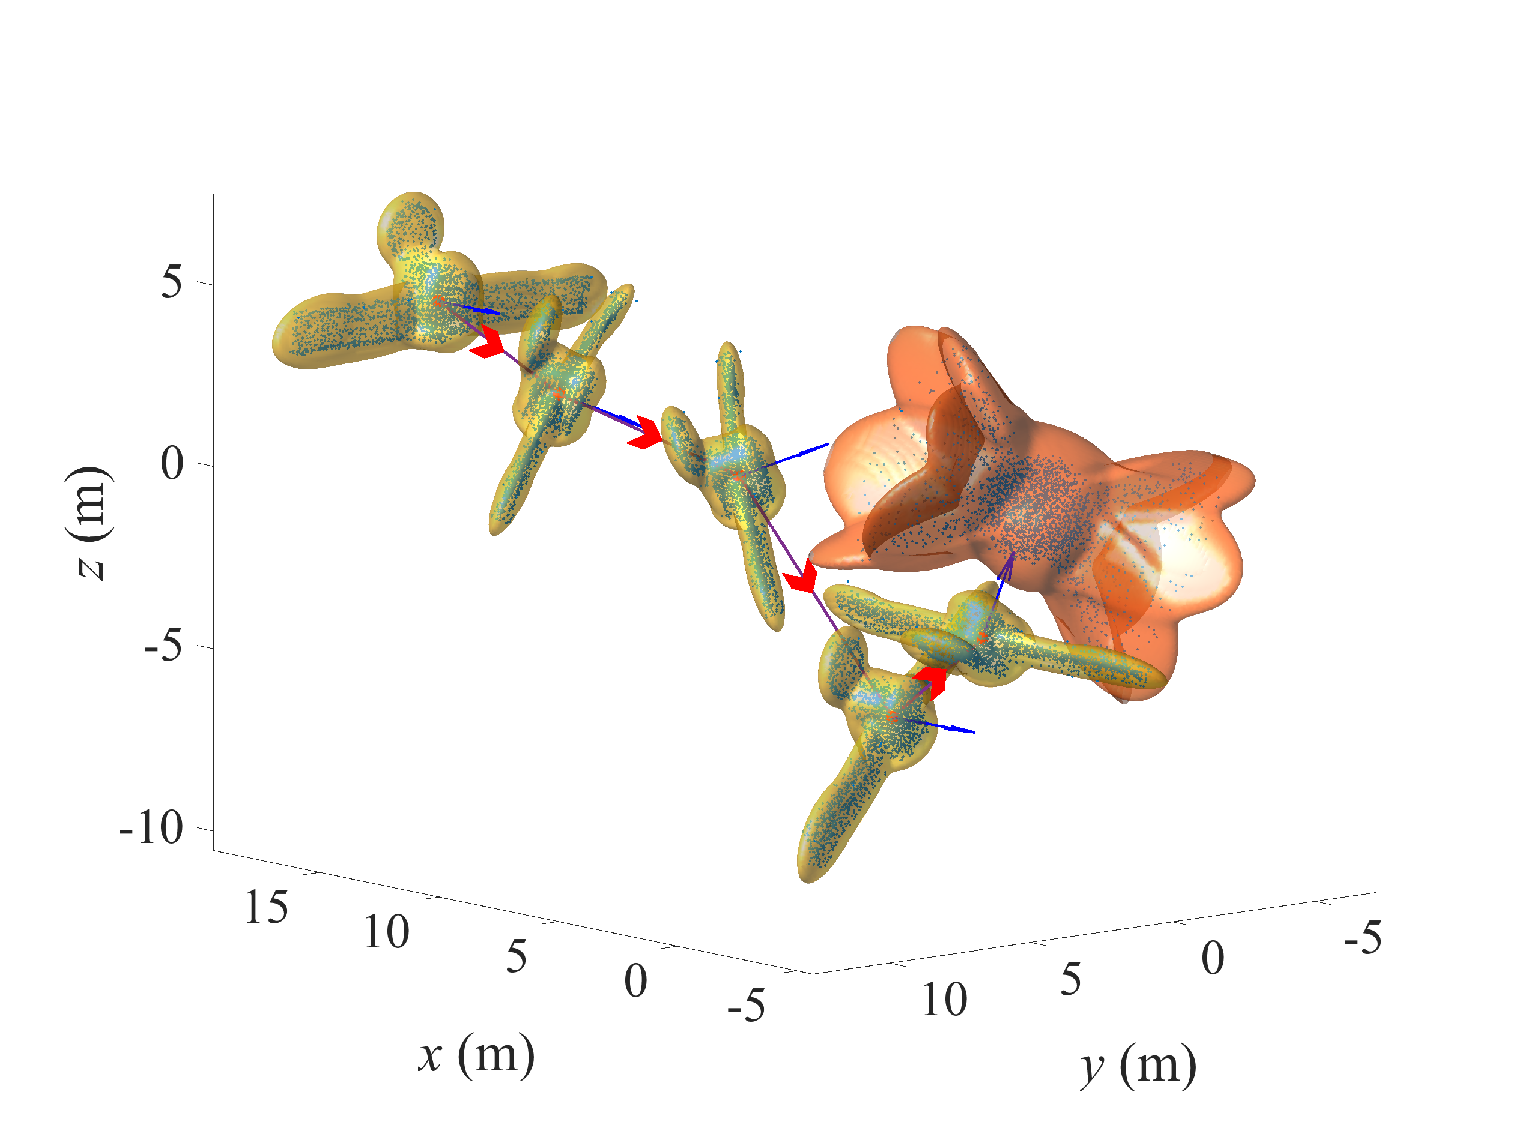
\includegraphics[width = 2.95in]{picture/FMT_path.pdf}
			\caption{服务星极近距离逼近参考路径\label{fig.fmtpath}}
		\end{subfigure}\hfill
		\begin{subfigure}[t]{0.47\textwidth}
			\centering
			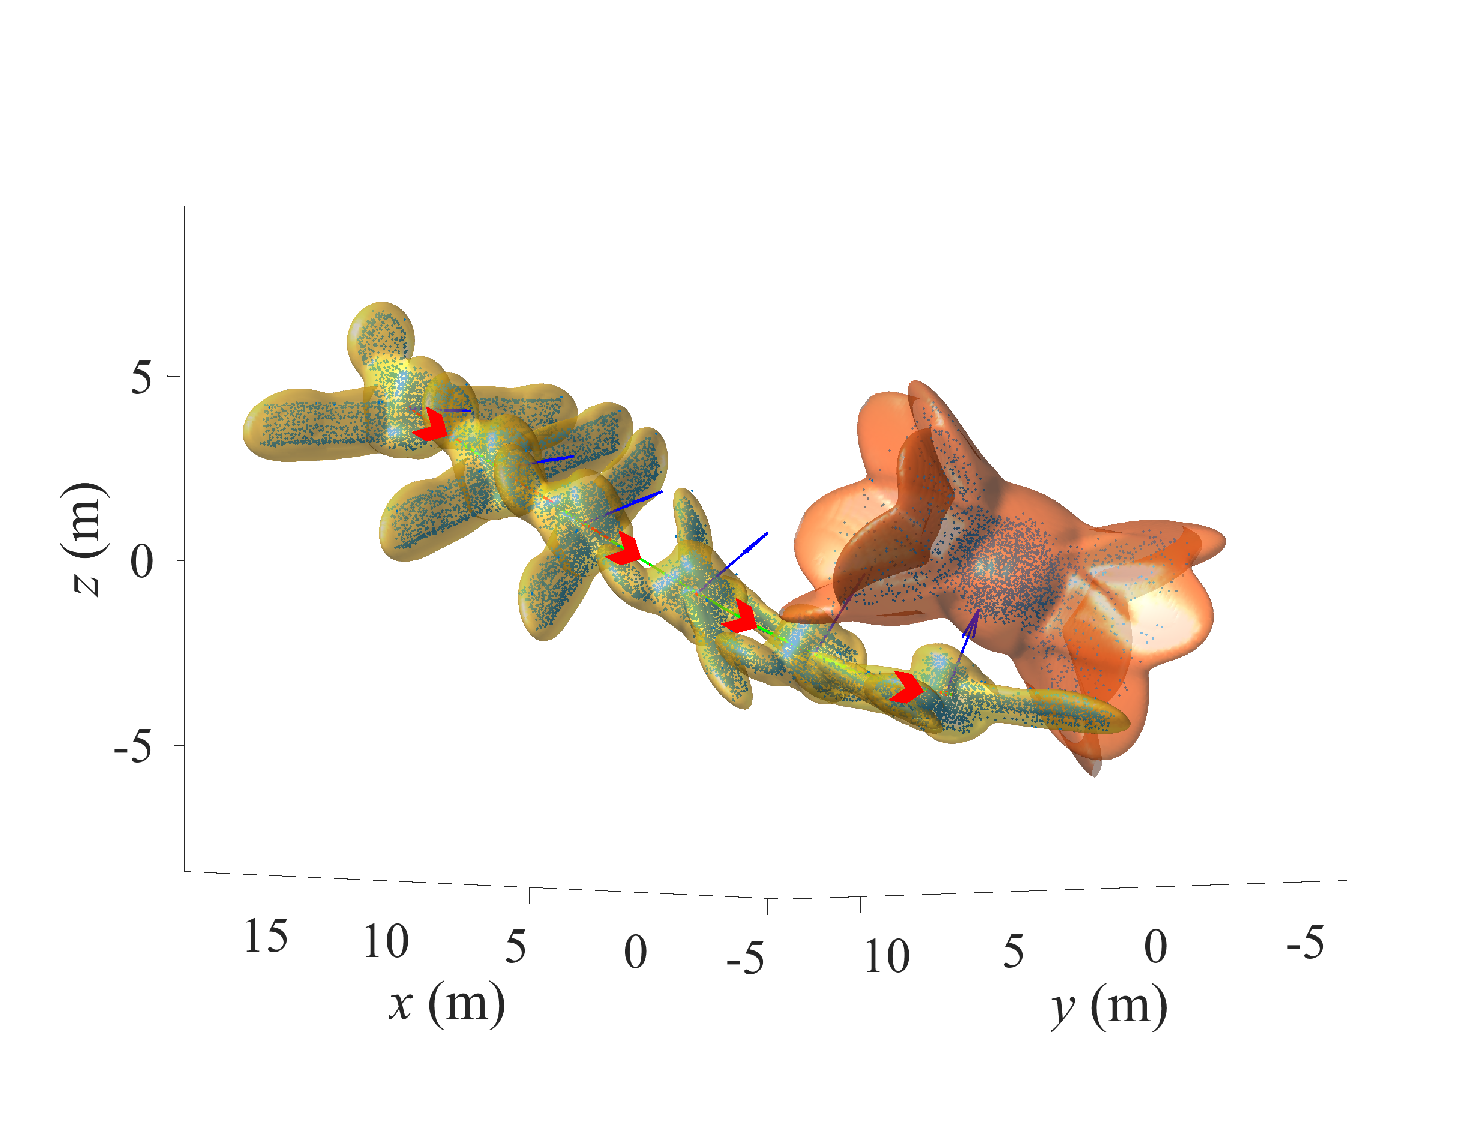
\includegraphics[width = 2.95in]{picture/proximity_tra.pdf}
			\caption{服务星极近距离逼近最终轨迹\label{fig.proximity-tra}}
		\end{subfigure}
	\end{minipage}
	\caption{服务星极近距离逼近轨迹\label{Fig.proximity-tra}}
\end{figure*}

%\begin{figure}[htbp]
%	\centering
%	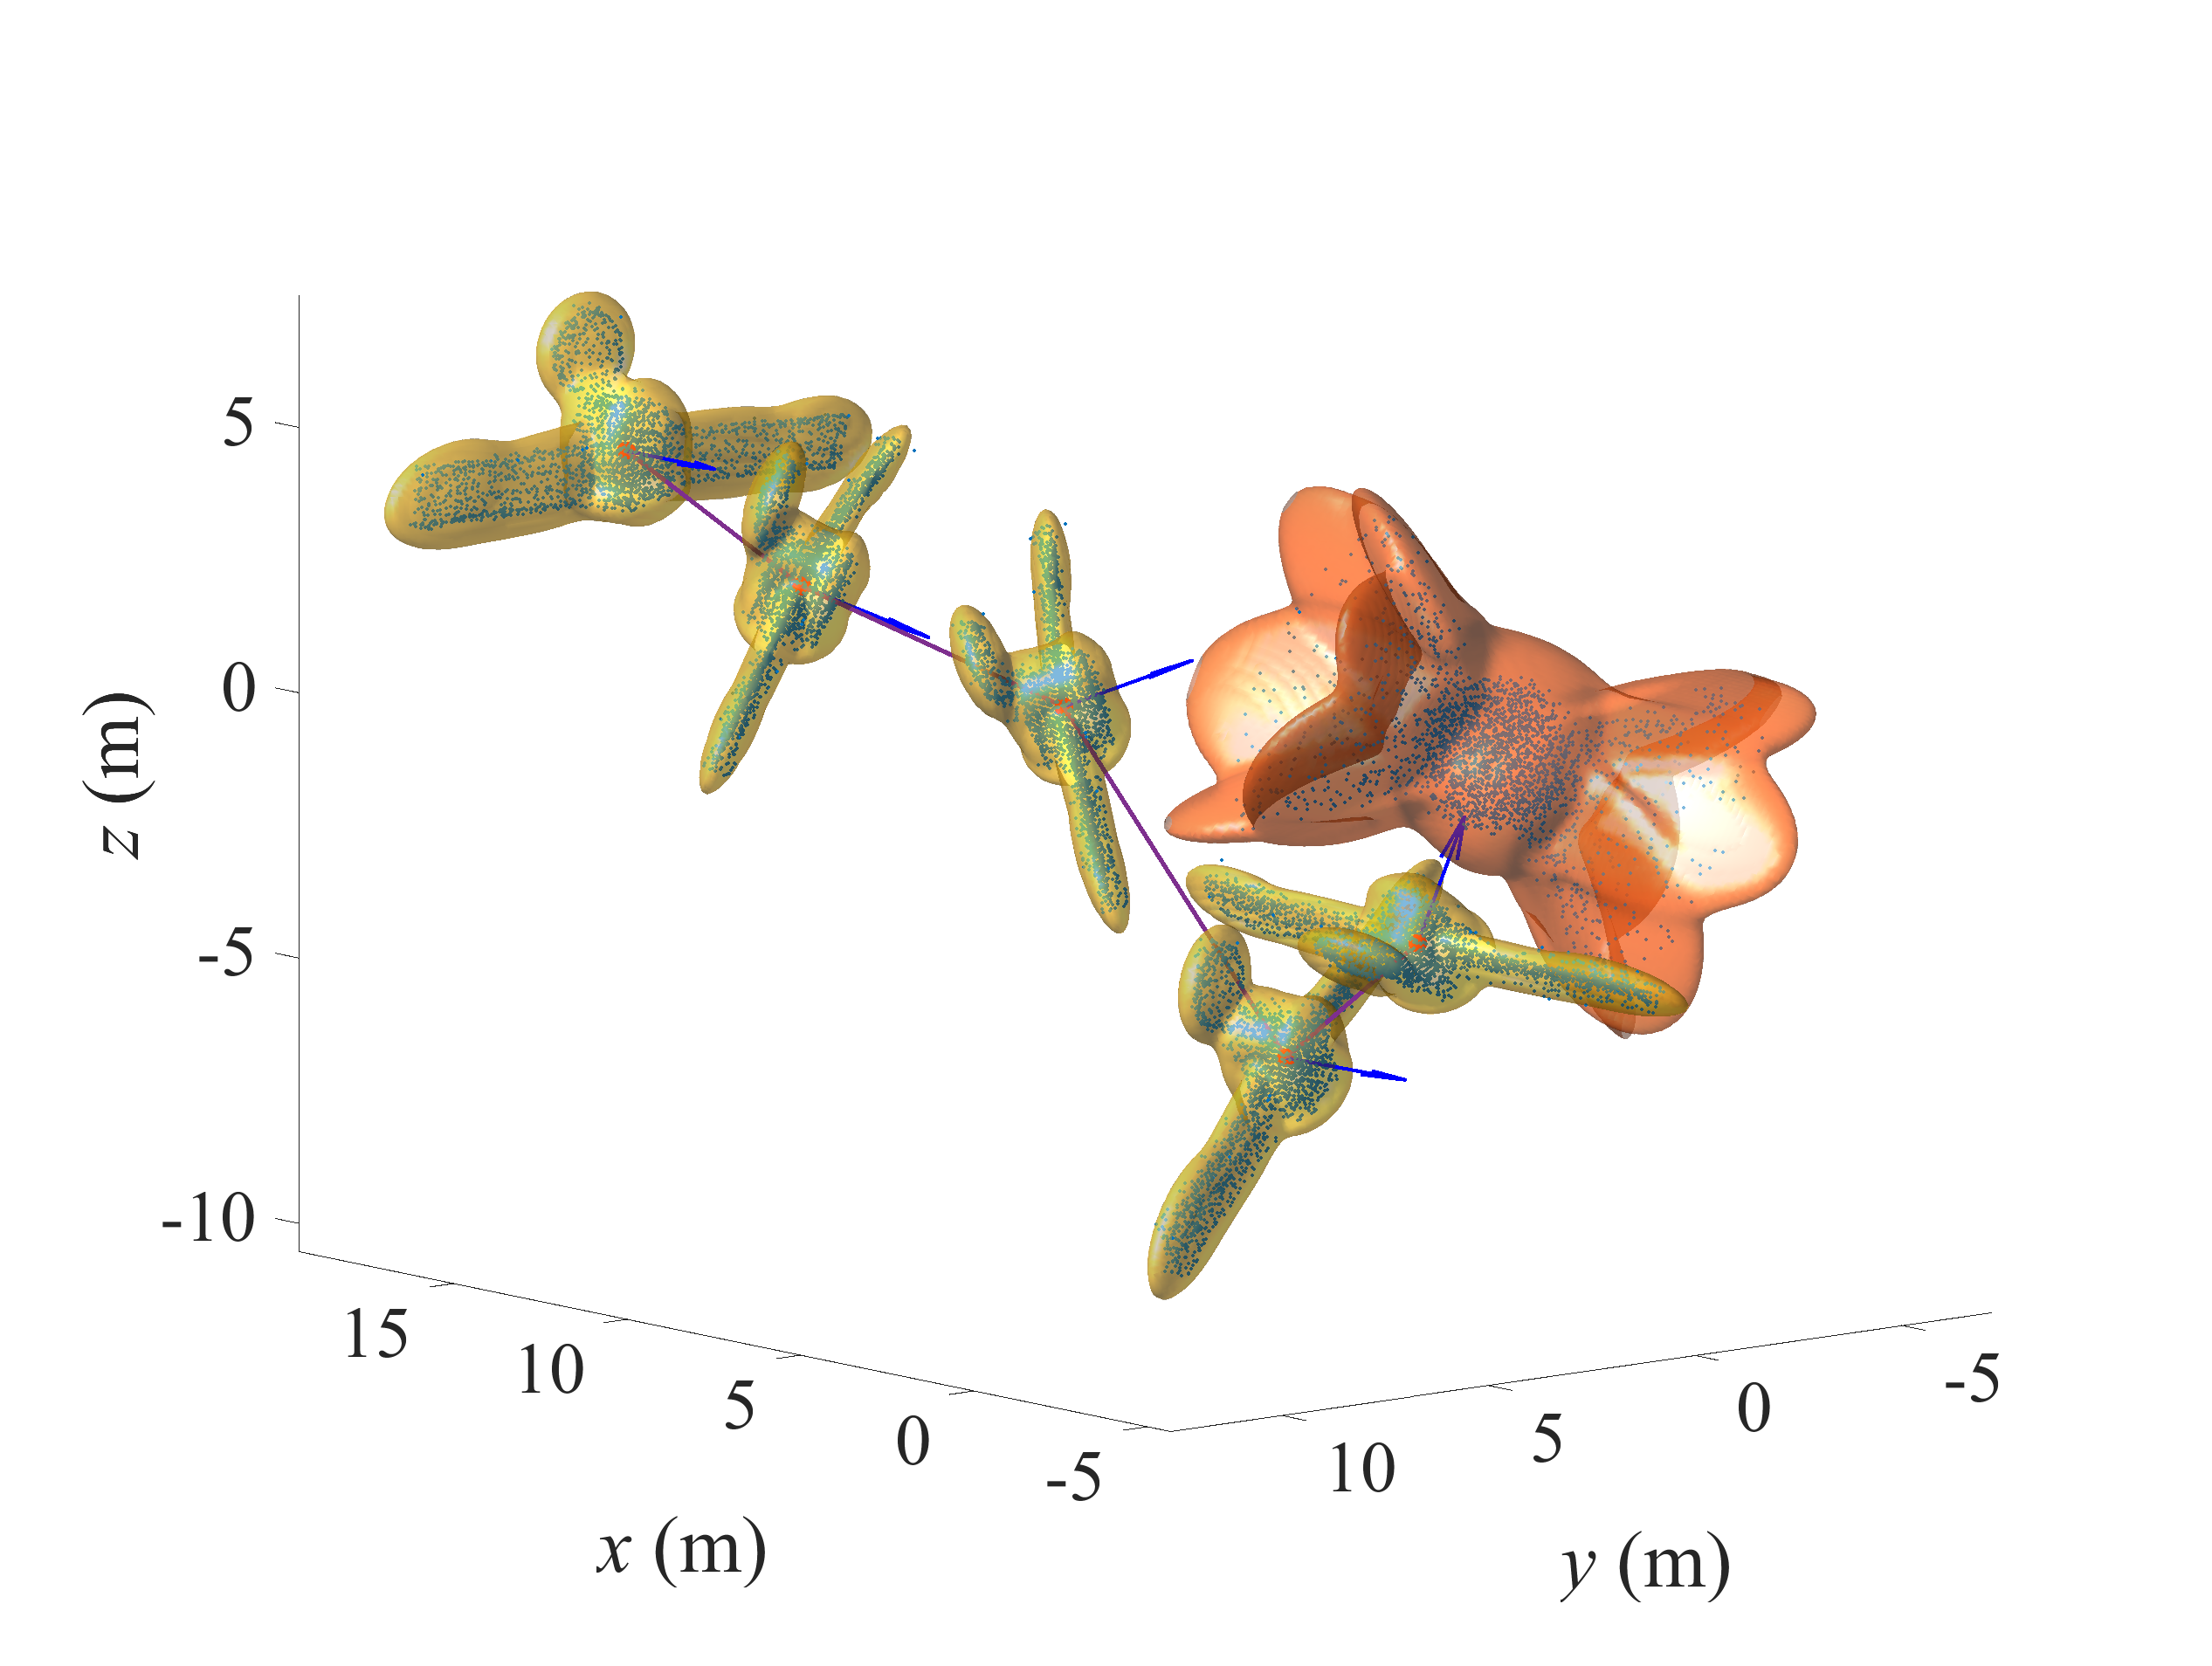
\includegraphics[width= 3.55 in]{picture/FMT_path.eps}
%	\caption{服务星极近距离逼近参考路径}
%	\label{fig.fmt-path}
%\end{figure}
%\begin{figure}[htbp]
%	\centering
%	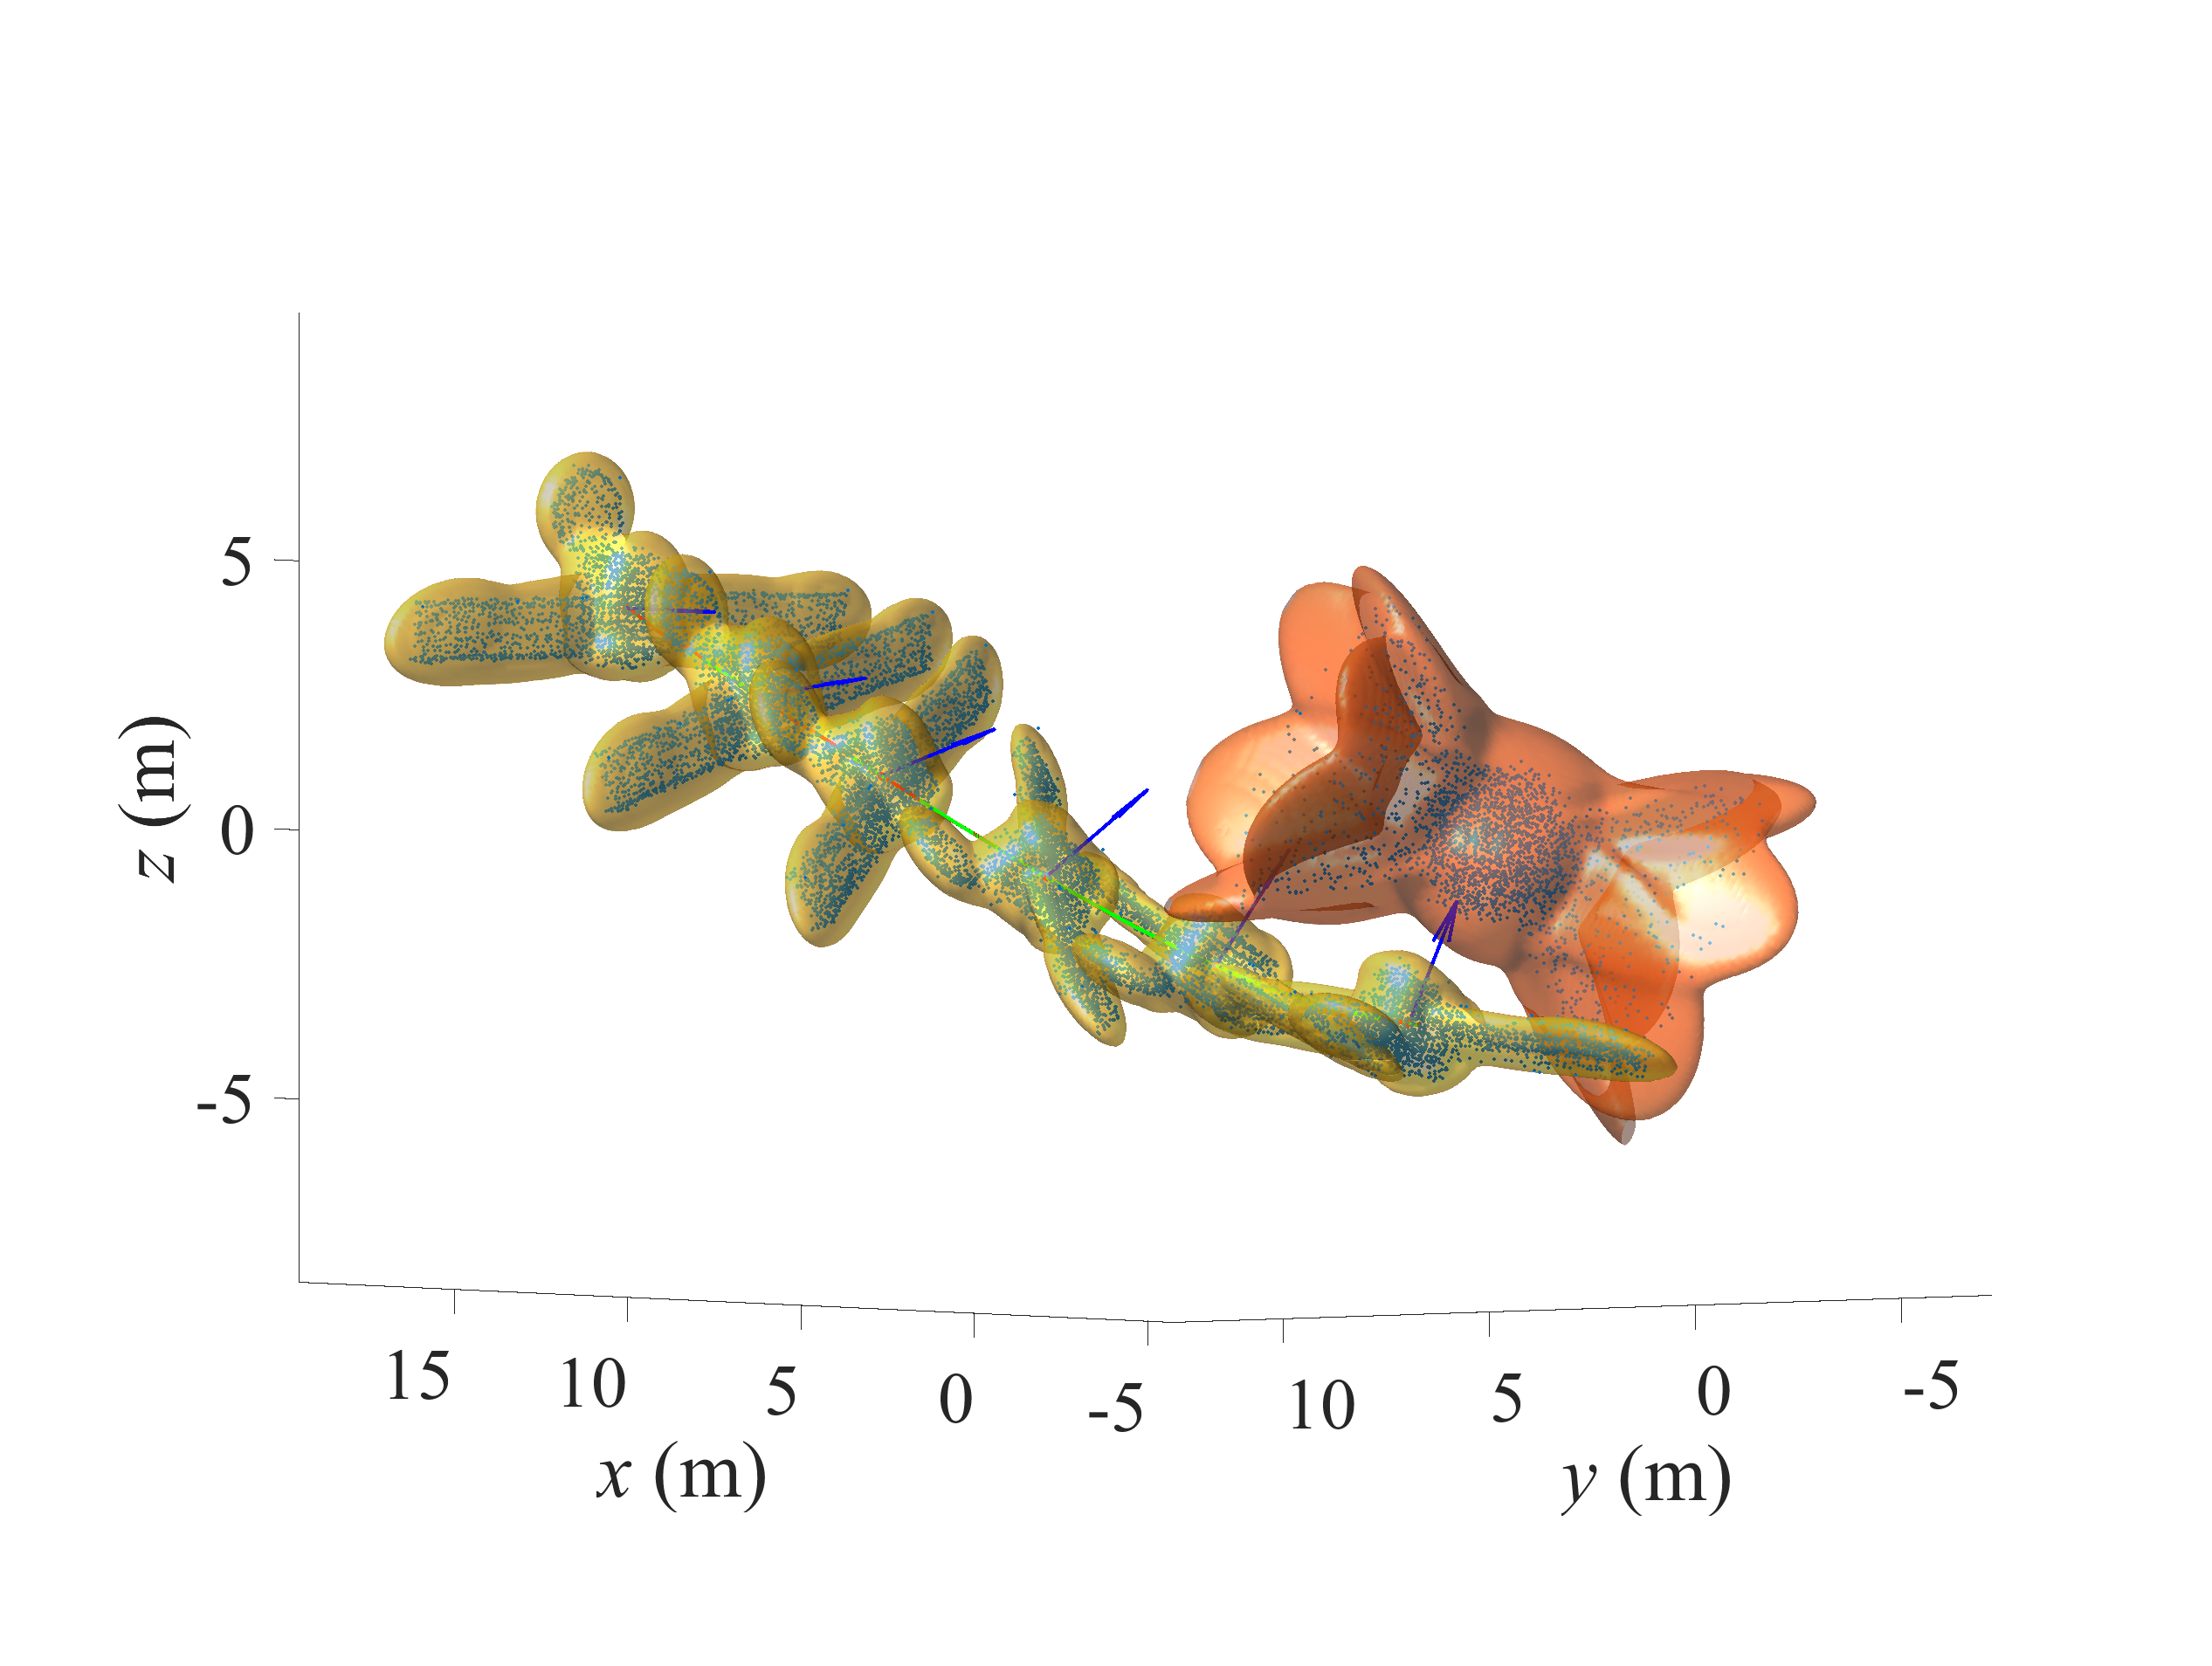
\includegraphics[width= 3.55 in]{picture/proximity_tra.eps}
%	\caption{服务星极近距离逼近最终轨迹}
%	\label{fig.proximity-tra}
%\end{figure}

逼近过程中碰撞危险度$P_c$及其阈值$P_{ts}$的变化情况如图\ref{fig.Ps_pts}所示,各轨迹点处碰撞危险度均小于阈值,故给出的逼近轨迹能保证服务星不与章动目标碰撞。

\begin{figure}[htb!]
	\centering
	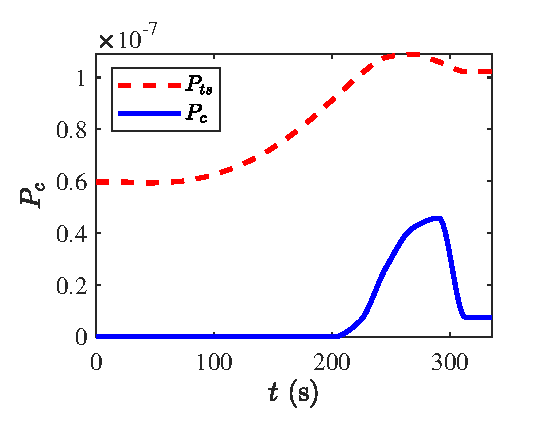
\includegraphics[width= 3.55 in]{picture/pts_ps.eps}
	\caption{逼近过程碰撞危险度变化情况}
	\label{fig.Ps_pts}
\end{figure}

逼近轨迹的速度、角速度变化如图\ref{fig:proximi_vec}所示,加速度、角加速度变化如图\ref{fig:proximi_acc}所示,各轨迹点处的速度、加速度、角速度、角加速度均满足限制要求。同时,为验证方法具有速度平滑效果,去除速度平滑项给出对比轨迹,其速度变化情况如图\ref{fig:proximi_vec}中点划线所示。可以看出,具有速度平滑项的轨迹速度波动明显小于对比轨迹,有助于减少服务星的燃料消耗。
%\begin{figure*}[htb!]
%	\centering
%	\begin{minipage}[t]{0.96\textwidth}
%		\centering
%		\begin{subfigure}[t]{0.47\textwidth}
%			\centering
%			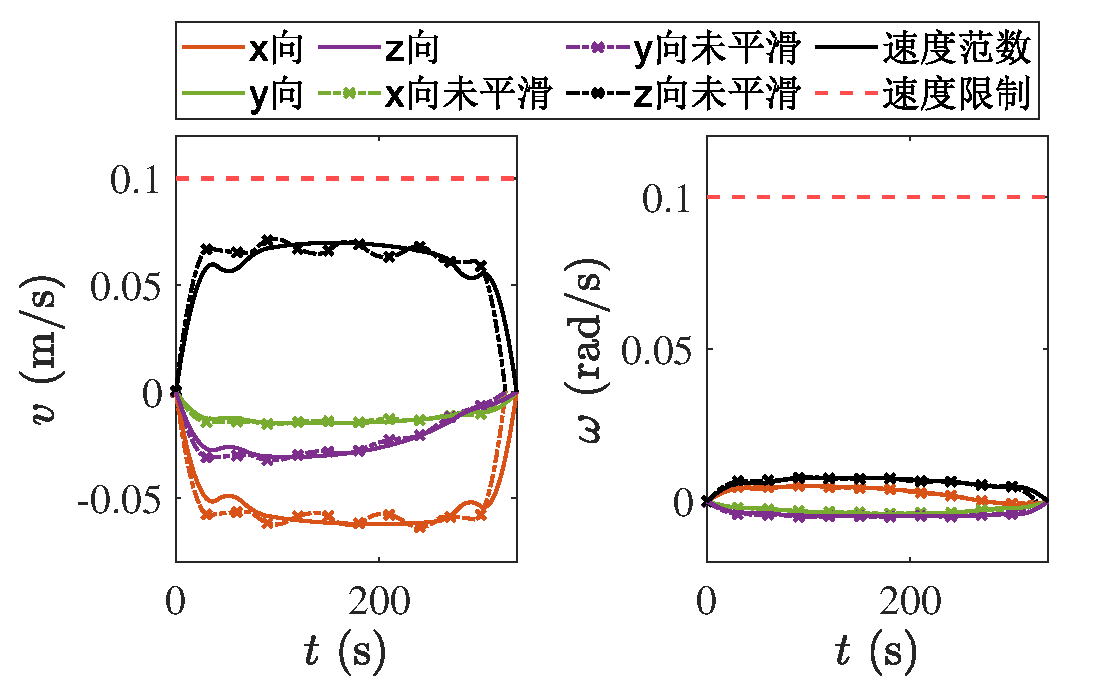
\includegraphics[width = 2.6in]{picture/proximity_vec_all.eps}
%			\caption{ }
%			\label{fig:proximi_vec}
%		\end{subfigure}\hfill
%		\begin{subfigure}[t]{0.47\textwidth}
%			\centering
%			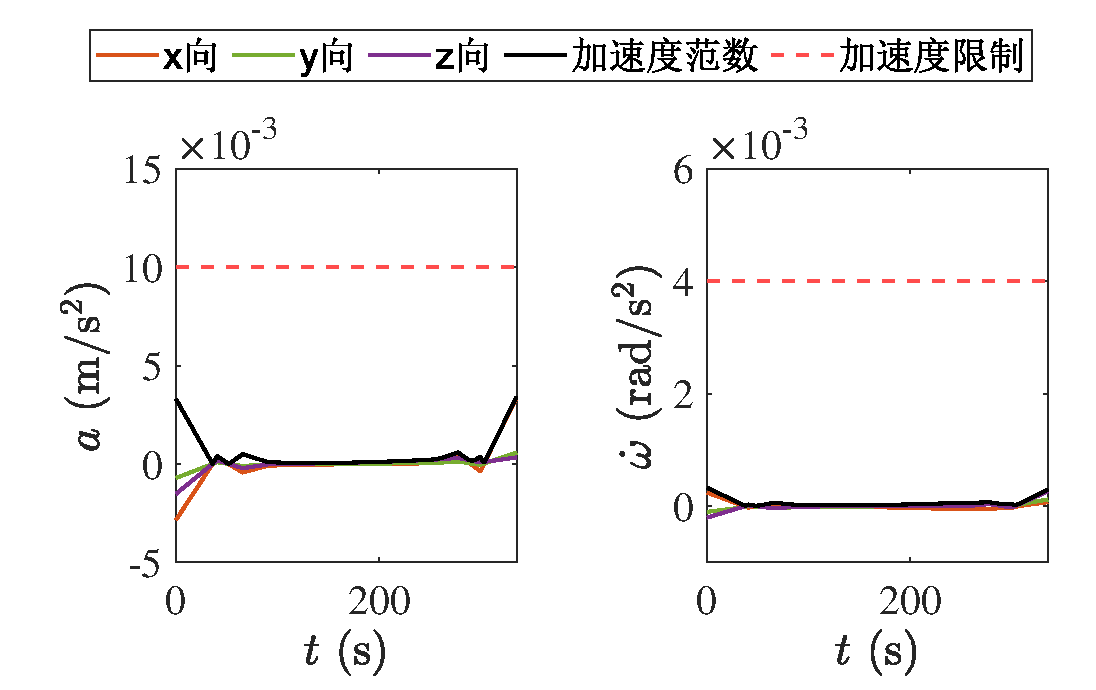
\includegraphics[width = 2.6in]{picture/proximity_acc_all.eps}
%			\caption{ }
%			\label{fig:proximi_acc}
%		\end{subfigure}
%	\end{minipage}
%	\caption{逼近过程服务星速度、加速度变化\label{Fig:proximi_vec}}
%\end{figure*}

\begin{figure}[htb!]
	\centering
	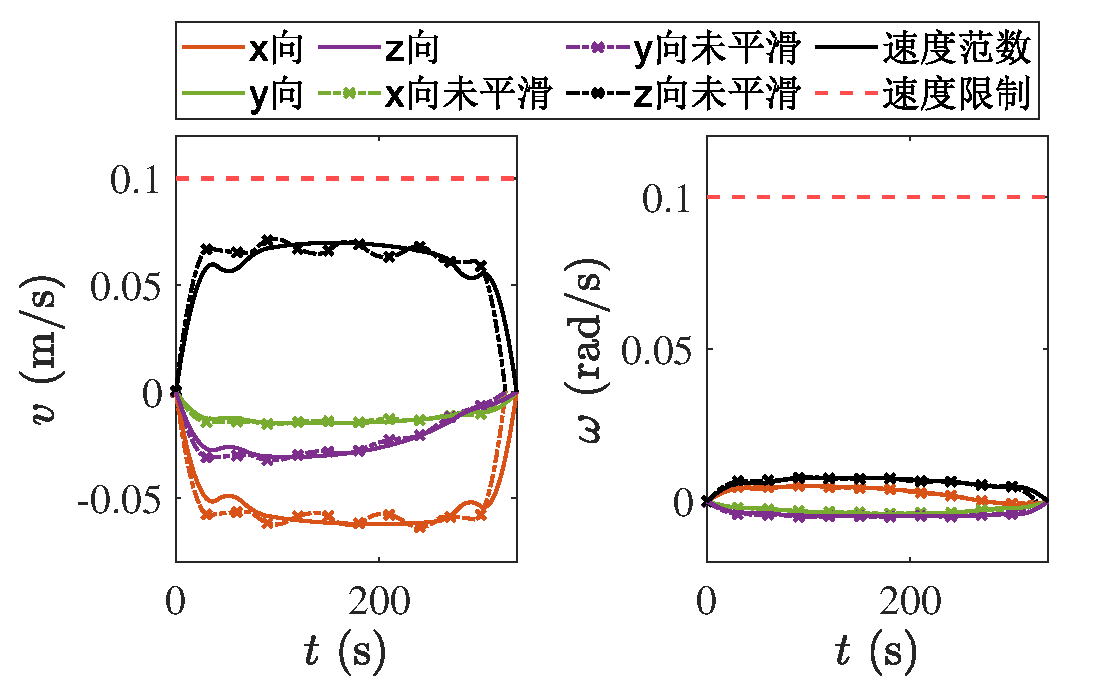
\includegraphics[width = 4.2in]{picture/proximity_vec_all.eps}
	\caption{逼近过程服务星速度变化情况}
	\label{fig:proximi_vec}
\end{figure}

\begin{figure}[htb!]
	\centering
	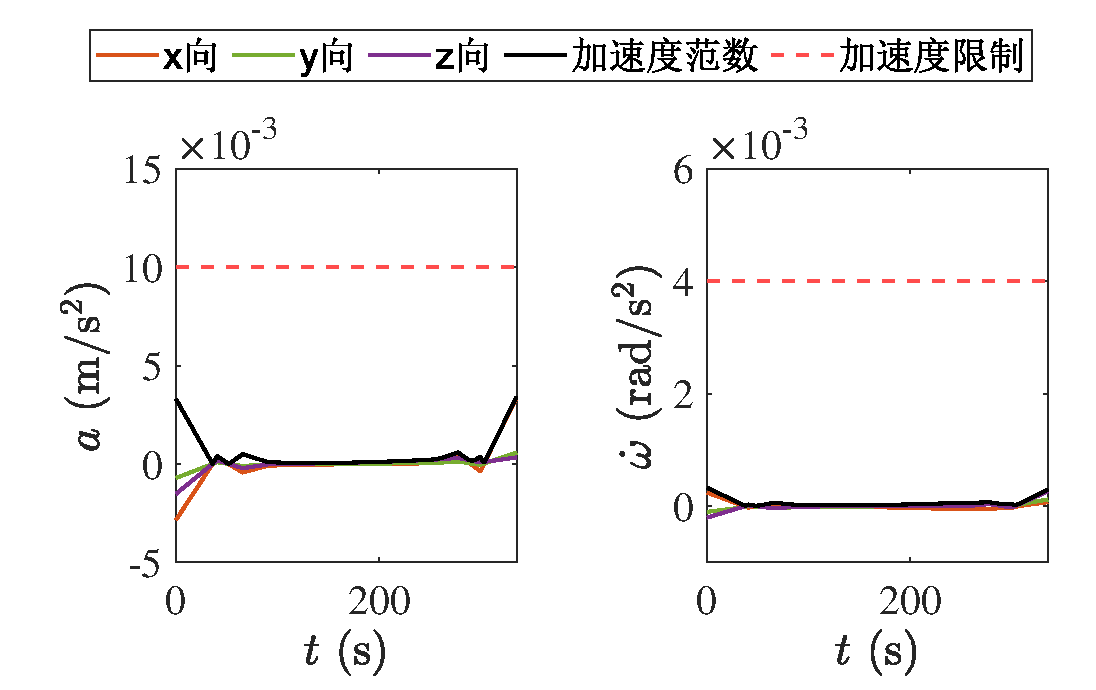
\includegraphics[width = 4.2in]{picture/proximity_acc_all.eps}
	\caption{逼近过程加速度变化情况}
	\label{fig:proximi_acc}
\end{figure}

到达期望位姿后,服务星开启磁场对章动目标进行消旋,规定当目标章动角变化超过$2\  (^\circ)$时需对章动区域点云${\mathbb{X}_F}$及其混合高斯模型${G_F}({{\boldsymbol{x}}^{\mathcal{L}}}|{\Theta _F})$进行更新,并通过所提出的消旋阶段位姿轨迹规划方法给出服务星的机动轨迹。当目标角速度降至$1.5\ (\mathrm{^\circ/s})$(直接抓捕允许的最大角速度)以下时消旋结束,消旋过程中服务星与章动目标间相对位姿变化情况如图\ref{Fig.detumble_pose}所示。其中,图\ref{Fig.detumble_pose}左下角轨迹表示消旋开始$1.72$小时后,最优消旋位姿变为垂直构型,服务星根据给出的轨迹机动至新的最优消旋位姿。

%其中,图\ref{Fig.detumble_pose}左下角轨迹表示消旋开始$1.72$小时后,最优消旋位姿变为垂直构型,服务星根据给出的轨迹机动至新的最优消旋位姿。

\begin{figure*}[htb!]
	\centering
	\begin{minipage}[t]{0.96\textwidth}
		\centering
		\begin{subfigure}[t]{0.47\textwidth}
			\centering
			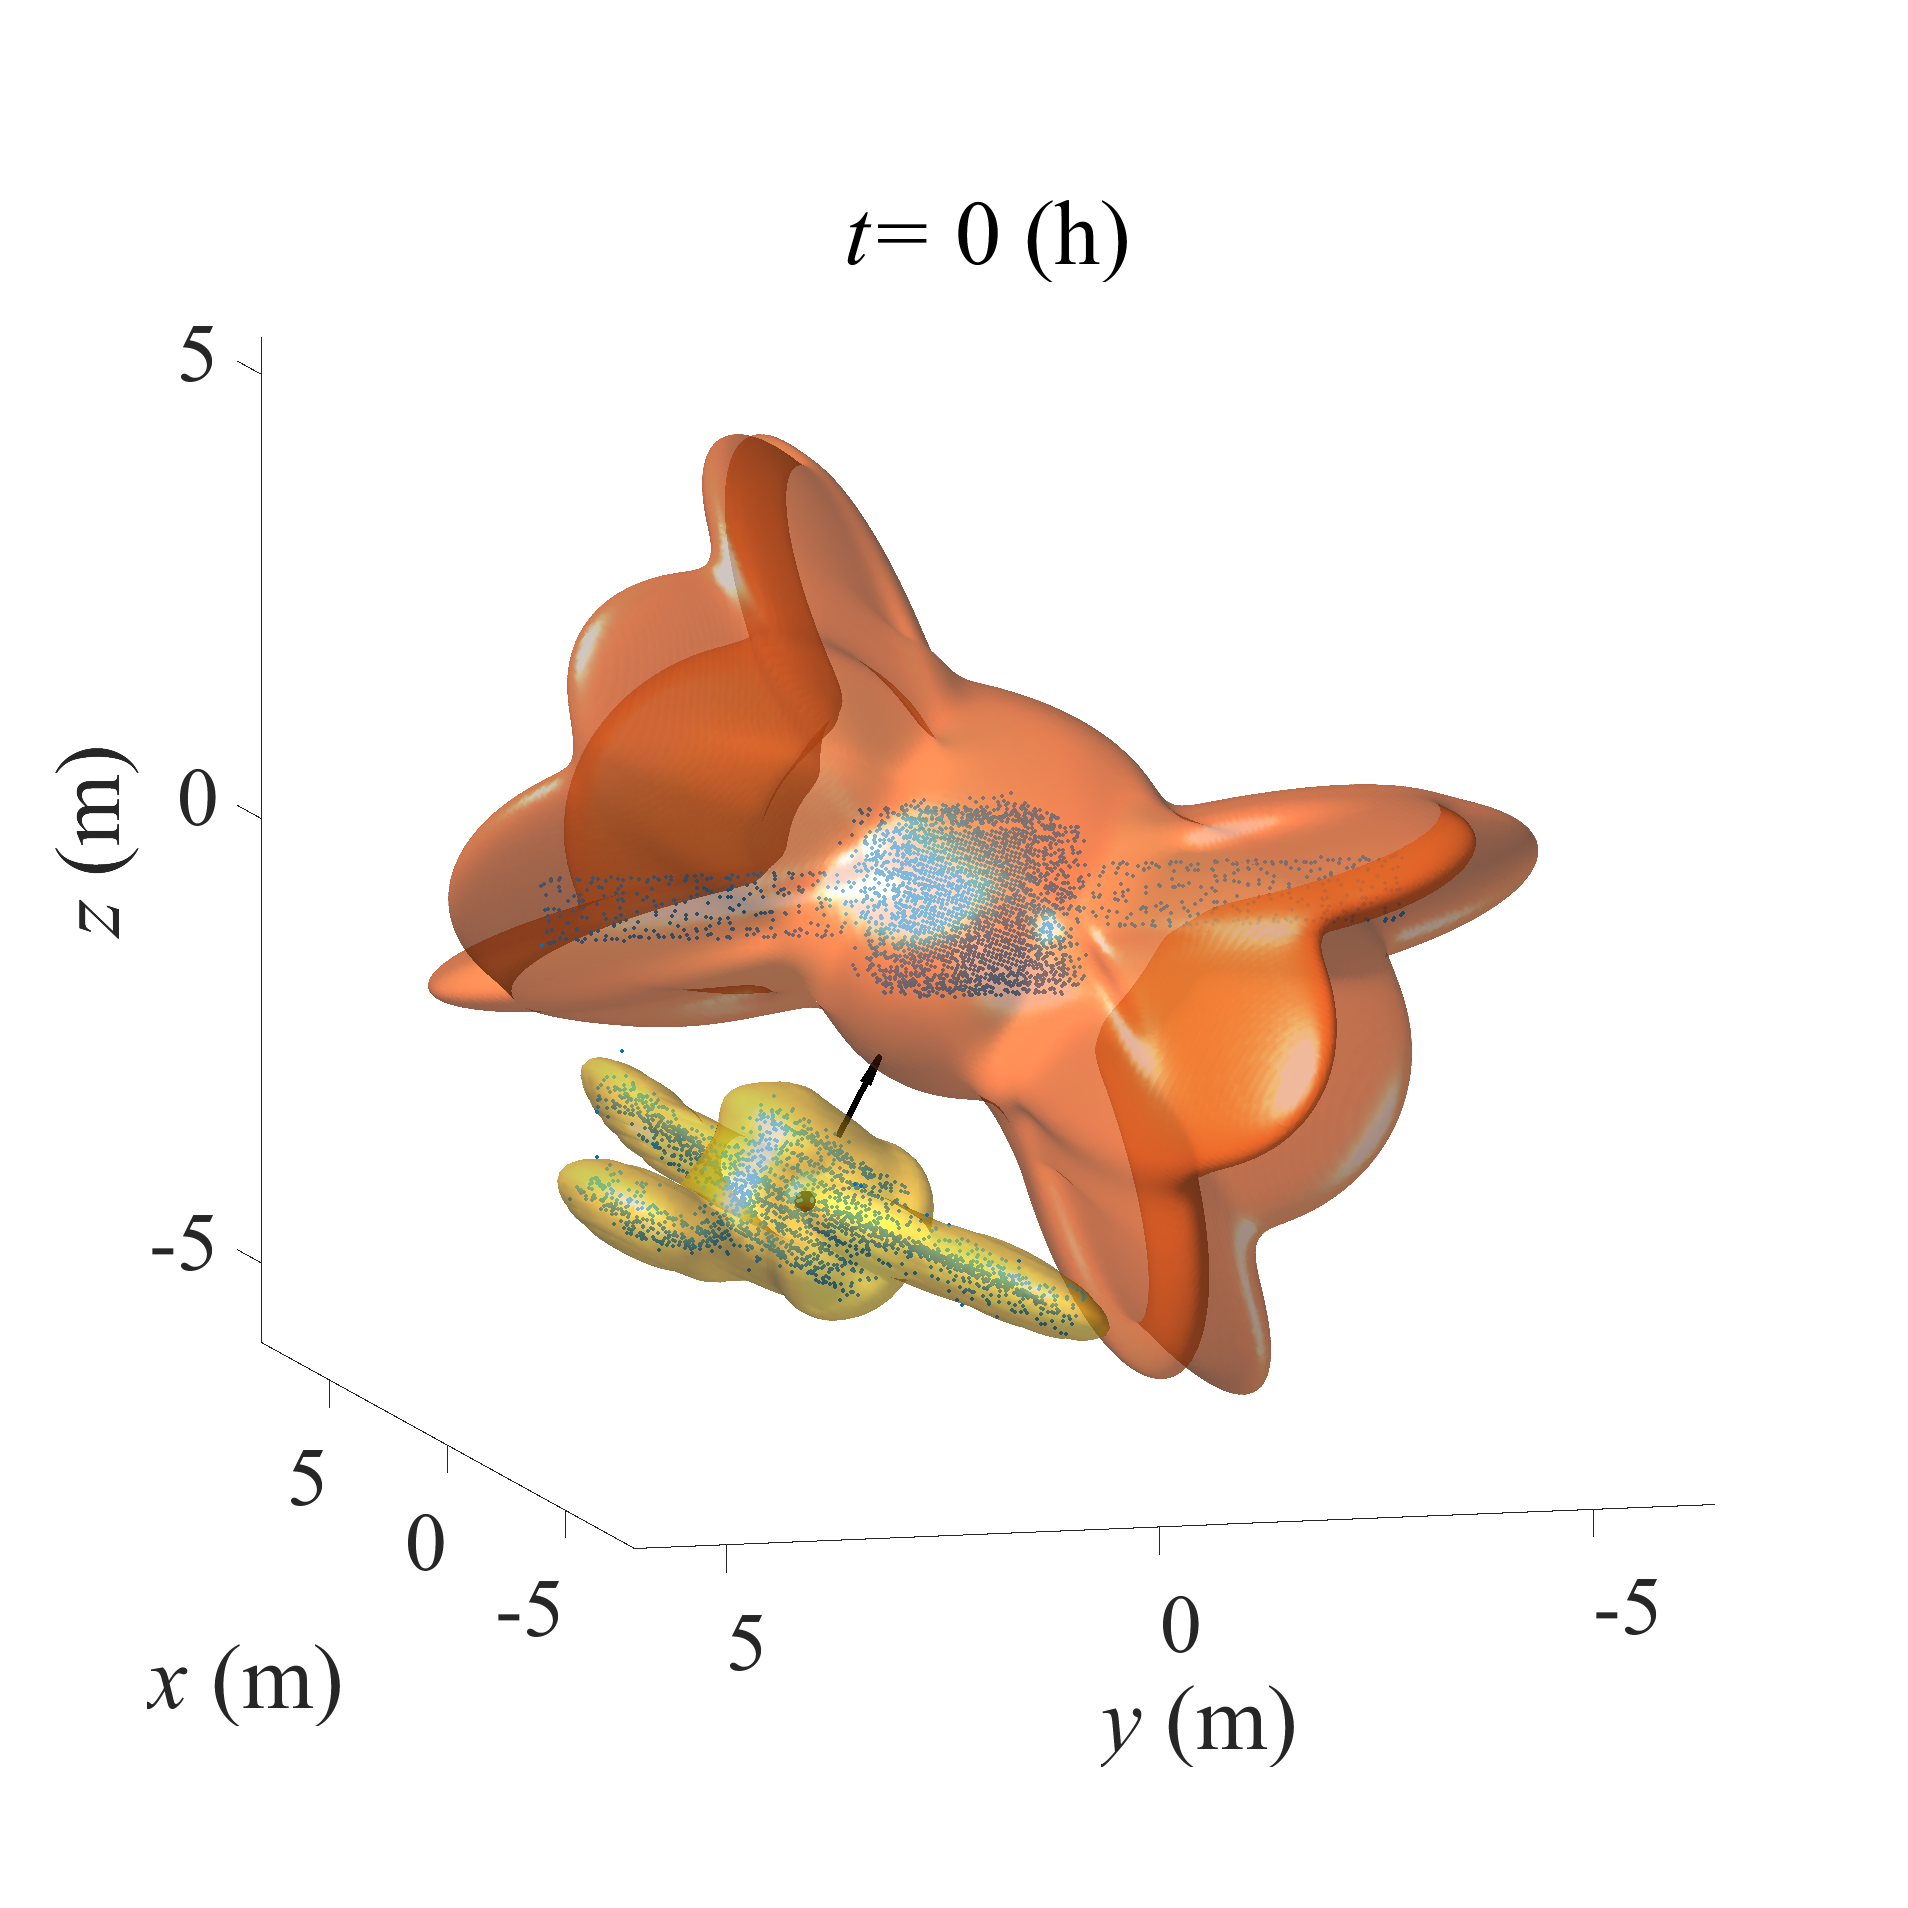
\includegraphics[width = 2.5in]{picture/detumble_time1.eps}
			\caption{ }
			\label{fig:detumbletime1}
		\end{subfigure}\hfill
		\begin{subfigure}[t]{0.47\textwidth}
			\centering
			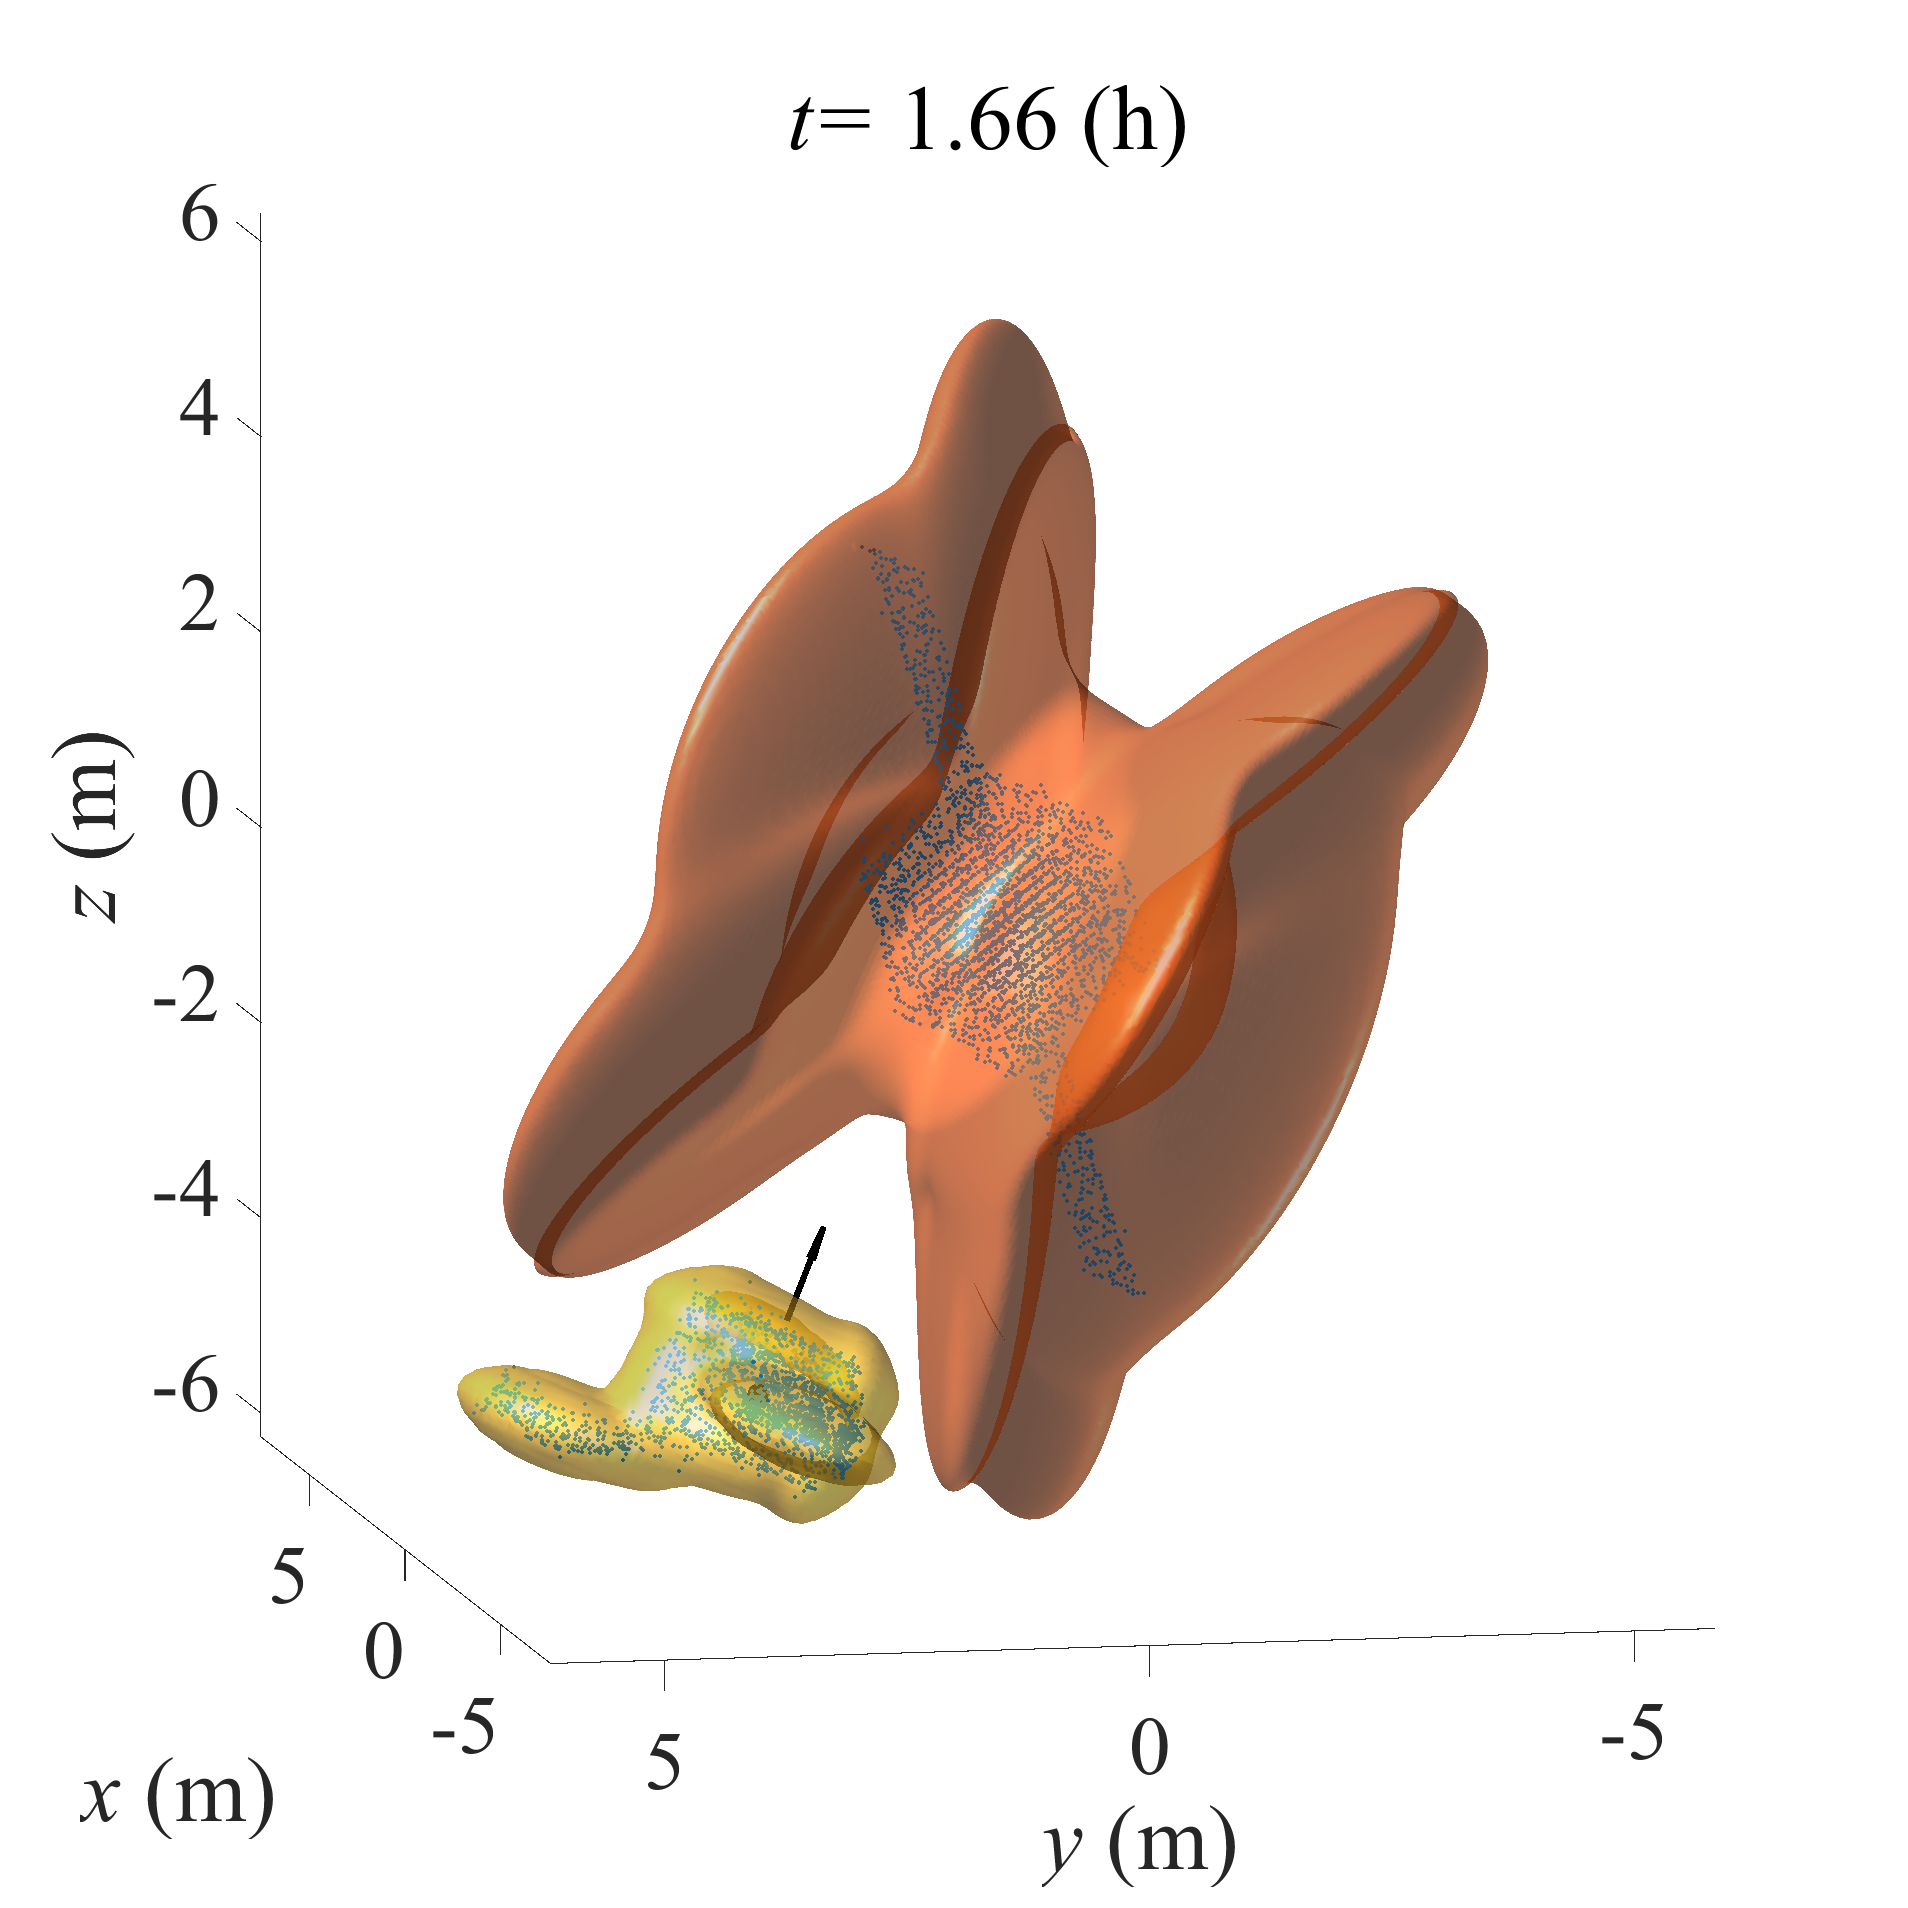
\includegraphics[width = 2.5in]{picture/detumble_time2.eps}
			\caption{ }
			\label{fig:detumbletime2}
		\end{subfigure}
		
		\vspace{10pt}
		\centering
		\begin{subfigure}[t]{0.47\textwidth}
			\centering
			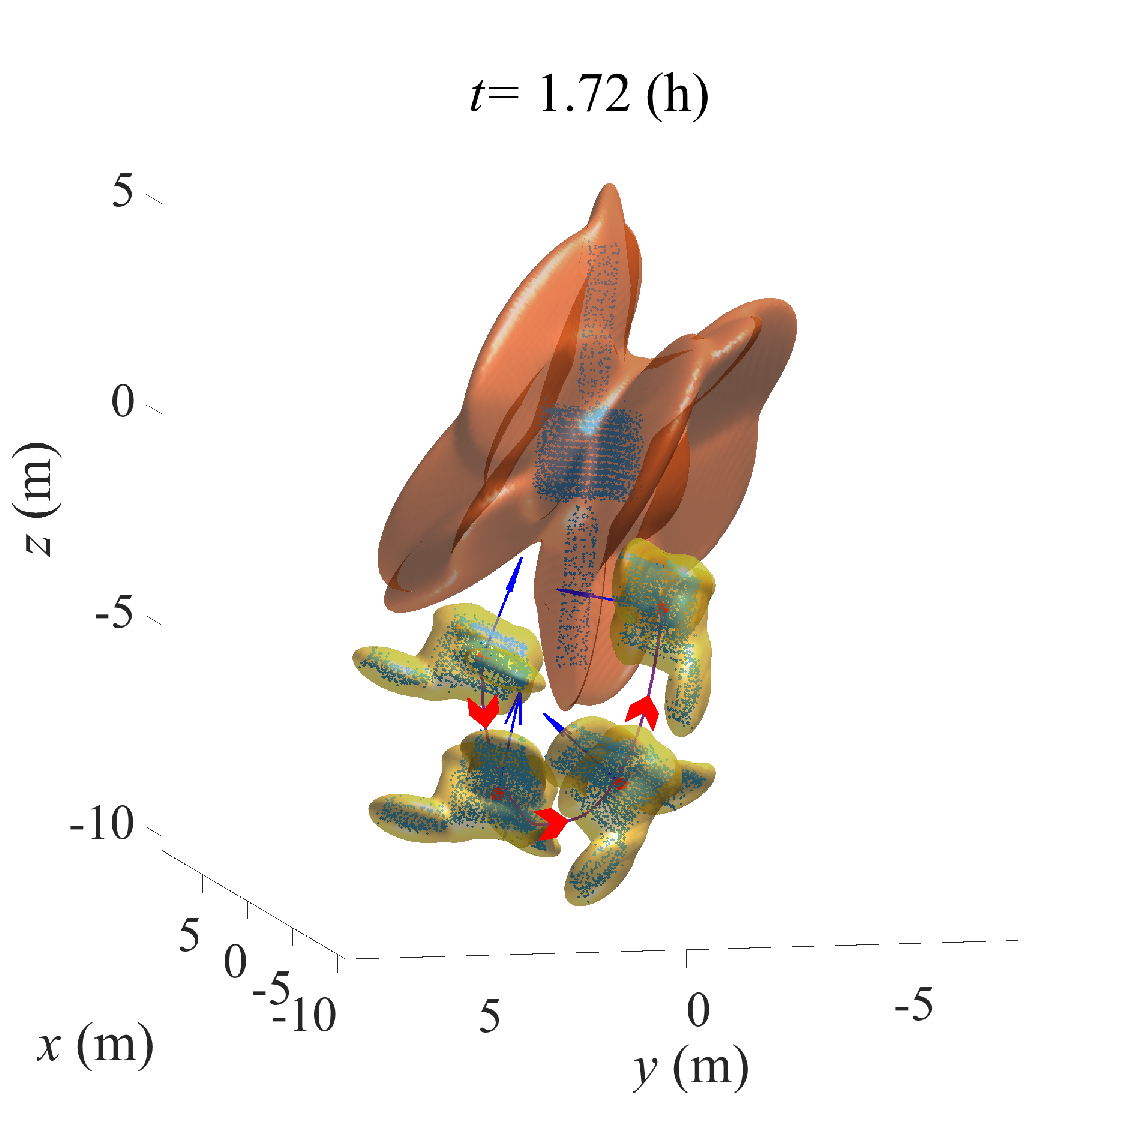
\includegraphics[width = 2.5in]{picture/detumble_tra.pdf}
			\caption{ }
			\label{fig:detumbletra}
		\end{subfigure}\hfill
		\begin{subfigure}[t]{0.47\textwidth}
			\centering
			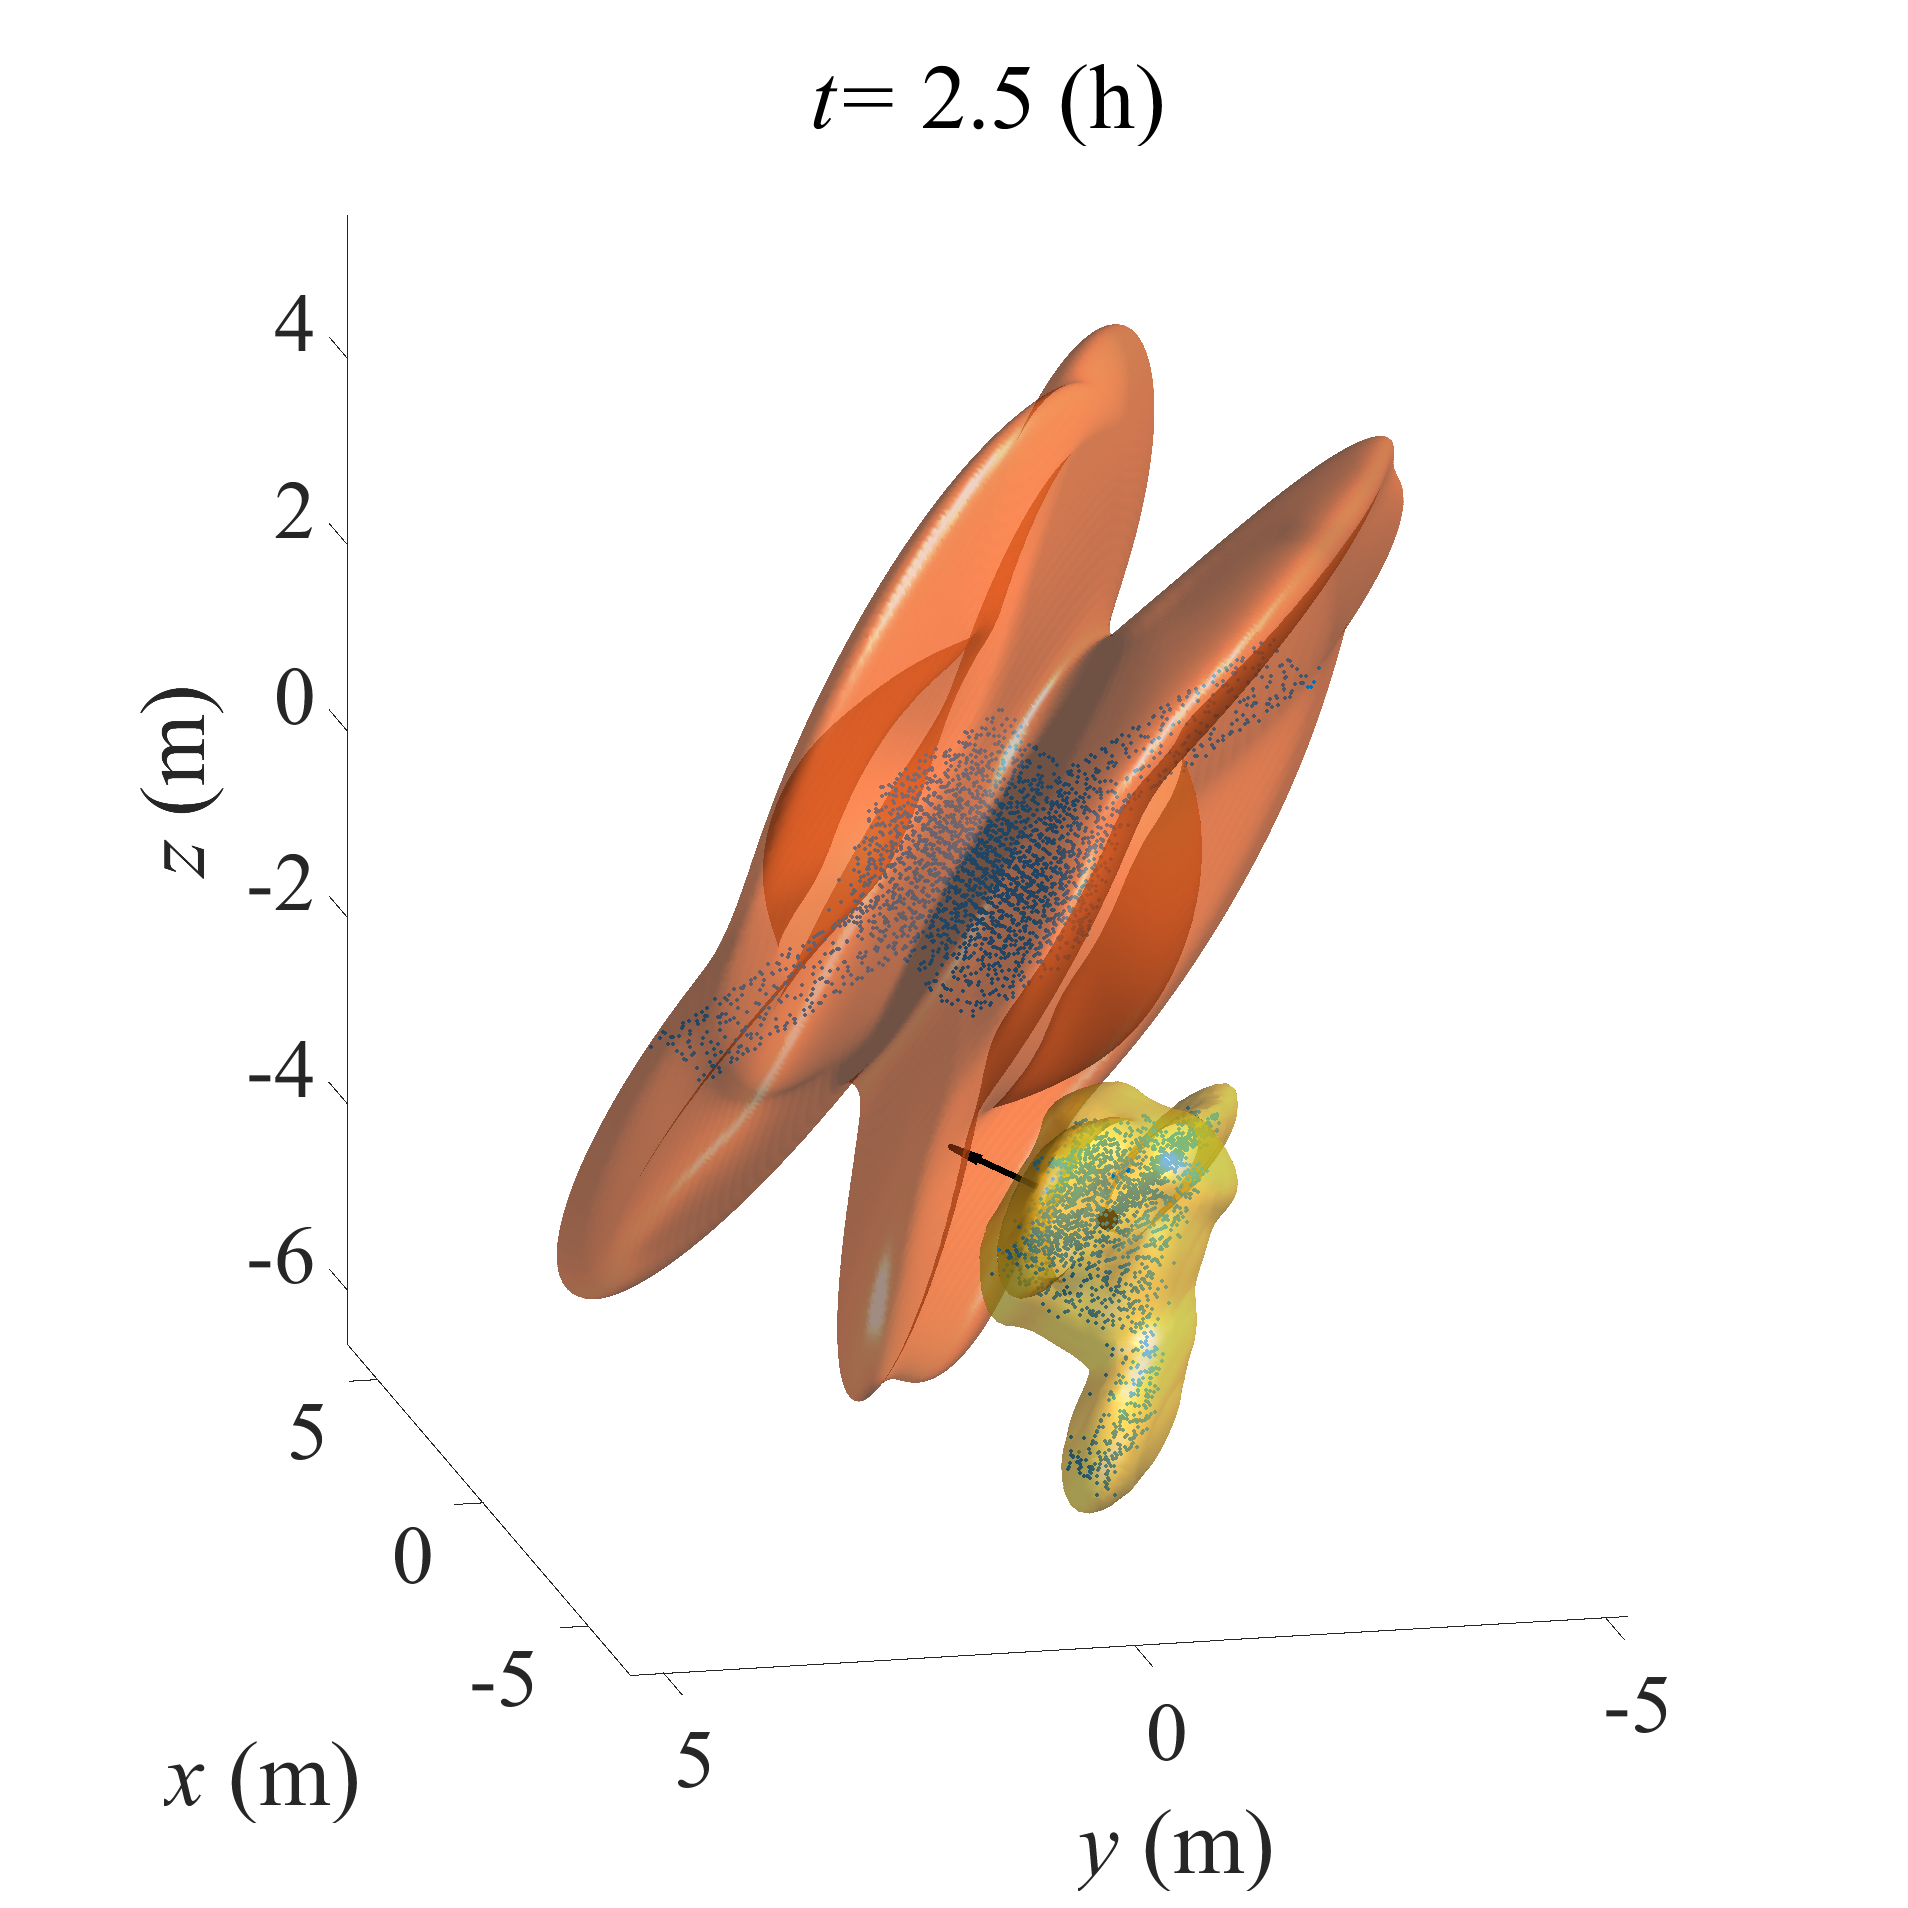
\includegraphics[width = 2.5in]{picture/detumble_time4.eps}
			\caption{ }
			\label{fig:detumbletime4}
		\end{subfigure}
	\end{minipage}
	\caption{切换构型消旋过程中的相对位姿情况\label{Fig.detumble_pose}}
\end{figure*}

消旋全过程中服务星相对位姿变化情况如图\ref{Fig.detumble_posiandpose}所示。可以看出,除$1.72\ (\mathrm{h})$时服务星从平行构型切换到垂直构型外,消旋过程中服务星位姿均无大幅变化,未因目标旋转进行不必要的机动。表明服务星所施加的消旋力矩始终平行目标角动量轴,使得目标角动量方向恒定,所提出的目标角动量定向安全区域能有效避免服务星的无效机动。
\begin{figure*}[htb!]
	\centering
	\begin{minipage}[t]{0.96\textwidth}
		\centering
		\begin{subfigure}[t]{0.47\textwidth}
			\centering
			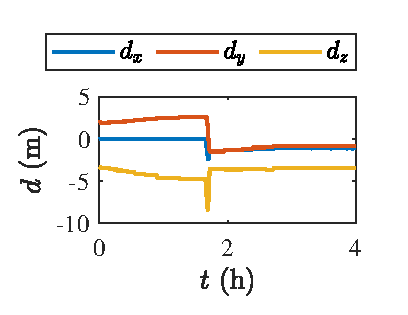
\includegraphics[width = 2.2in]{picture/detumble_posi.eps}
			\caption{ }
			\label{fig:detumbleposi}
		\end{subfigure}\hfill
		\begin{subfigure}[t]{0.47\textwidth}
			\centering
			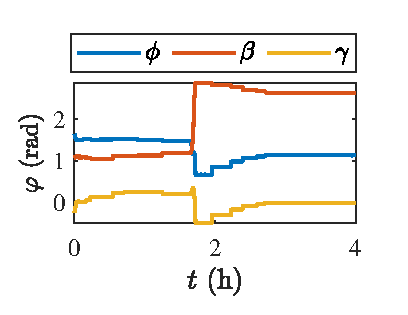
\includegraphics[width = 2.2in]{picture/detumble_pose.eps}
			\caption{ }
			\label{fig:detumblepose}
		\end{subfigure}
	\end{minipage}
	\caption{惯性系下服务星相对位置与欧拉角变化情况\label{Fig.detumble_posiandpose}}
\end{figure*}

消旋过程中服务星的速度、角速度变化情况如图\ref{Fig.detumble_Vec_C}所示,而加速度、角加速度变化情况如图\ref{Fig.detumble_Acc_C}所示。从图中可以看出,整个消旋过程中,服务星的速度、加速度等均满足约束条件,表明轨迹各控制点处速度、加速度等均小于限制值,算法\ref{retime}可行有效,所给出的消旋轨迹服务星可执行。
%\begin{figure*}[htb!]
%	\centering
%	\begin{minipage}[t]{0.96\textwidth}
%		\centering
%		\begin{subfigure}[t]{0.23\textwidth}
%			\centering
%			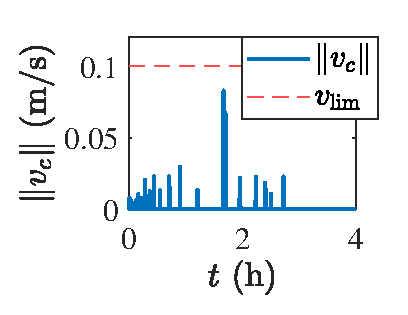
\includegraphics[width = 1.475in]{picture/chaser_detumble_vec.eps}
%			\caption{ }
%			\label{fig:detumble_vec_c}
%		\end{subfigure}\hfill
%		\begin{subfigure}[t]{0.23\textwidth}
%			\centering
%			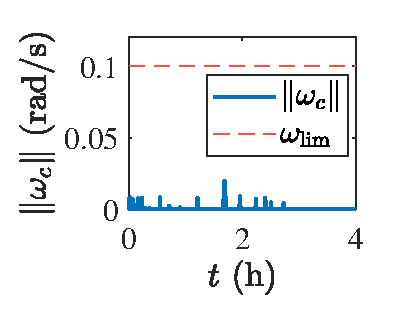
\includegraphics[width = 1.475in]{picture/chaser_detumble_ang_vec.eps}
%			\caption{ }
%			\label{fig:detumble_angvec_c}
%		\end{subfigure}\hfill
%		\begin{subfigure}[t]{0.23\textwidth}
%			\centering
%			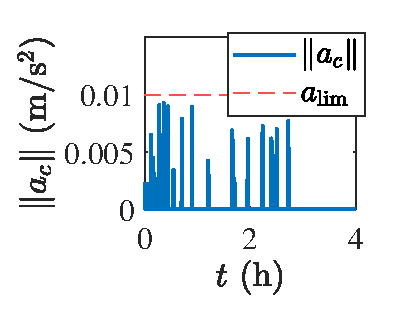
\includegraphics[width = 1.475in]{picture/chaser_detumble_acc.eps}
%			\caption{ }
%			\label{fig:detumble_acc_c}
%		\end{subfigure}\hfill
%		\begin{subfigure}[t]{0.23\textwidth}
%			\centering
%			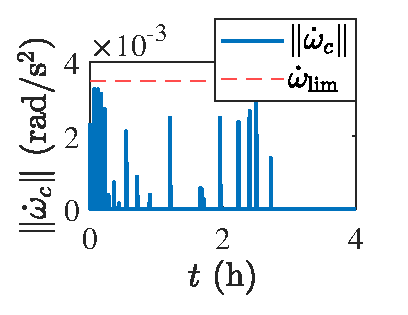
\includegraphics[width = 1.475in]{picture/chaser_detumble_ang_acc.eps}
%			\caption{ }
%			\label{fig:detumble_angacc_c}
%		\end{subfigure}
%	\end{minipage}
%	\caption{惯性系下服务星速度及角速度变化情况\label{Fig.detumble_Vec_C}}
%\end{figure*}
\begin{figure*}[htb!]
	\centering
	\begin{minipage}[t]{0.96\textwidth}
		\centering
		\begin{subfigure}[t]{0.47\textwidth}
			\centering
			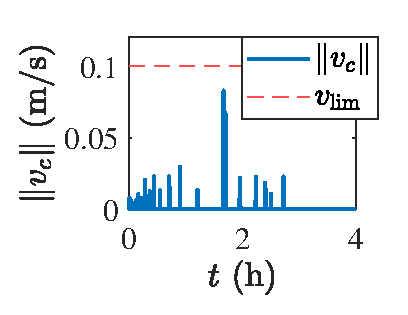
\includegraphics[width = 2.2in]{picture/chaser_detumble_vec.eps}
			\caption{ }
			\label{fig:detumble_vec_c}
		\end{subfigure}\hfill
		\begin{subfigure}[t]{0.47\textwidth}
			\centering
			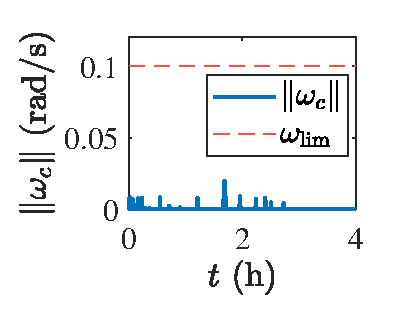
\includegraphics[width = 2.2in]{picture/chaser_detumble_ang_vec.eps}
			\caption{ }
			\label{fig:detumble_angvec_c}
		\end{subfigure}\hfill
	\end{minipage}
	\caption{惯性系下服务星速度及角速度变化情况\label{Fig.detumble_Vec_C}}
\end{figure*}

\begin{figure*}[htb!]
	\centering
	\begin{minipage}[t]{0.96\textwidth}
			\centering
			\begin{subfigure}[t]{0.47\textwidth}
					\centering
					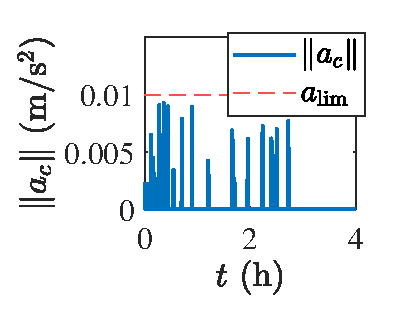
\includegraphics[width = 2.2in]{picture/chaser_detumble_acc.eps}
					\caption{ }
					\label{fig:detumble_acc_c}
				\end{subfigure}
			\begin{subfigure}[t]{0.47\textwidth}
					\centering
					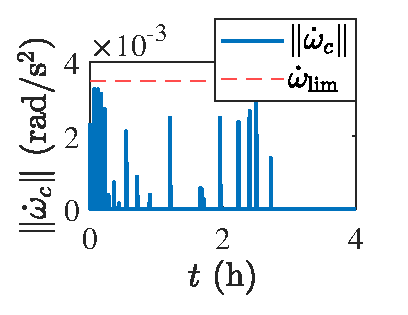
\includegraphics[width = 2.2in]{picture/chaser_detumble_ang_acc.eps}
					\caption{ }
					\label{fig:detumble_angacc_c}
				\end{subfigure}
		\end{minipage}
	\caption{惯性系下服务星加速度及角加速度变化情况\label{Fig.detumble_Acc_C}}
\end{figure*}

多次测试得消旋过程轨迹规划耗时如图\ref{Fig.PlantimeConsum}所示,规划最大耗时为$0.59\ (\mathrm{s})$,平均耗时为$0.38\ (\mathrm{s})$,由于目标章动角变化相对缓慢,故该耗时能满足消旋任务需求,可实现在线规划。

\begin{figure*}[htb!]
	\centering
	\begin{minipage}[t]{0.96\textwidth}
		\centering
		\begin{subfigure}[t]{0.47\textwidth}
			\centering
			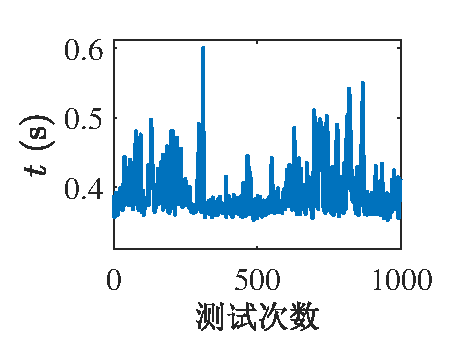
\includegraphics[width = 2.2in]{picture/plantimeconsum.eps}
			\caption{ }
			\label{fig:plantimeconsum}
		\end{subfigure}\hfill
		\begin{subfigure}[t]{0.47\textwidth}
			\centering
			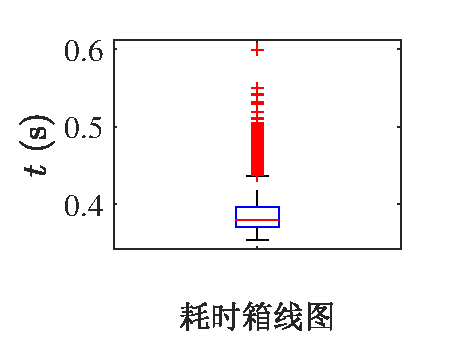
\includegraphics[width = 2.2in]{picture/plantimeconsum_boxline.eps}
			\caption{ }
			\label{fig:plantimeconsum_boxline}
		\end{subfigure}
	\end{minipage}
	\caption{消旋轨迹规划耗时\label{Fig.PlantimeConsum}}
\end{figure*}

随后,本文选取固定构型的消旋策略\cite{Liuprec2022}与采用椭球安全区域的固定位姿消旋策略\cite{gomezGuidanceNavigationControl2017}进行比较。其中,固定构型消旋策略仍采用本文提出的GMMCRA法确定安全位姿,但限定其构型为平行构型,服务星起始位姿为${\boldsymbol{x}}_{\mathcal{B}}^{\mathcal{N}}=\left[0.0025,1.934,-3.311\right]^{\top}$和${\boldsymbol{\varphi}}_{\mathcal{B}}^{\mathcal{N}}=\left[1.639,1.062,-0.247\right]^{\top}$,终止位姿为${\boldsymbol{x}}_{\mathcal{B}}^{\mathcal{N}}=\left[0,3.565,-6.416\right]^{\top}$和${\boldsymbol{\varphi}}_{\mathcal{B}}^{\mathcal{N}}=\left[1.511,1.161,0.231\right]^{\top}$。固定位姿消旋策略中服务星位姿始终为${\boldsymbol{x}}_{\mathcal{B}}^{\mathcal{N}}=\left[0,3.599,-6.477\right]^{\top}$和${\boldsymbol{\varphi}}_{\mathcal{B}}^{\mathcal{N}}=[1.511,1.161$ $,0.231]^{\top}$。这两种消旋策略下服务星的相对位姿情况如图\ref{Fig.posefix_detumble_pose}所示。
\begin{figure*}[htb!]
	\centering
	\begin{minipage}[t]{0.96\textwidth}
		\centering
		\begin{subfigure}[t]{0.47\textwidth}
			\centering
			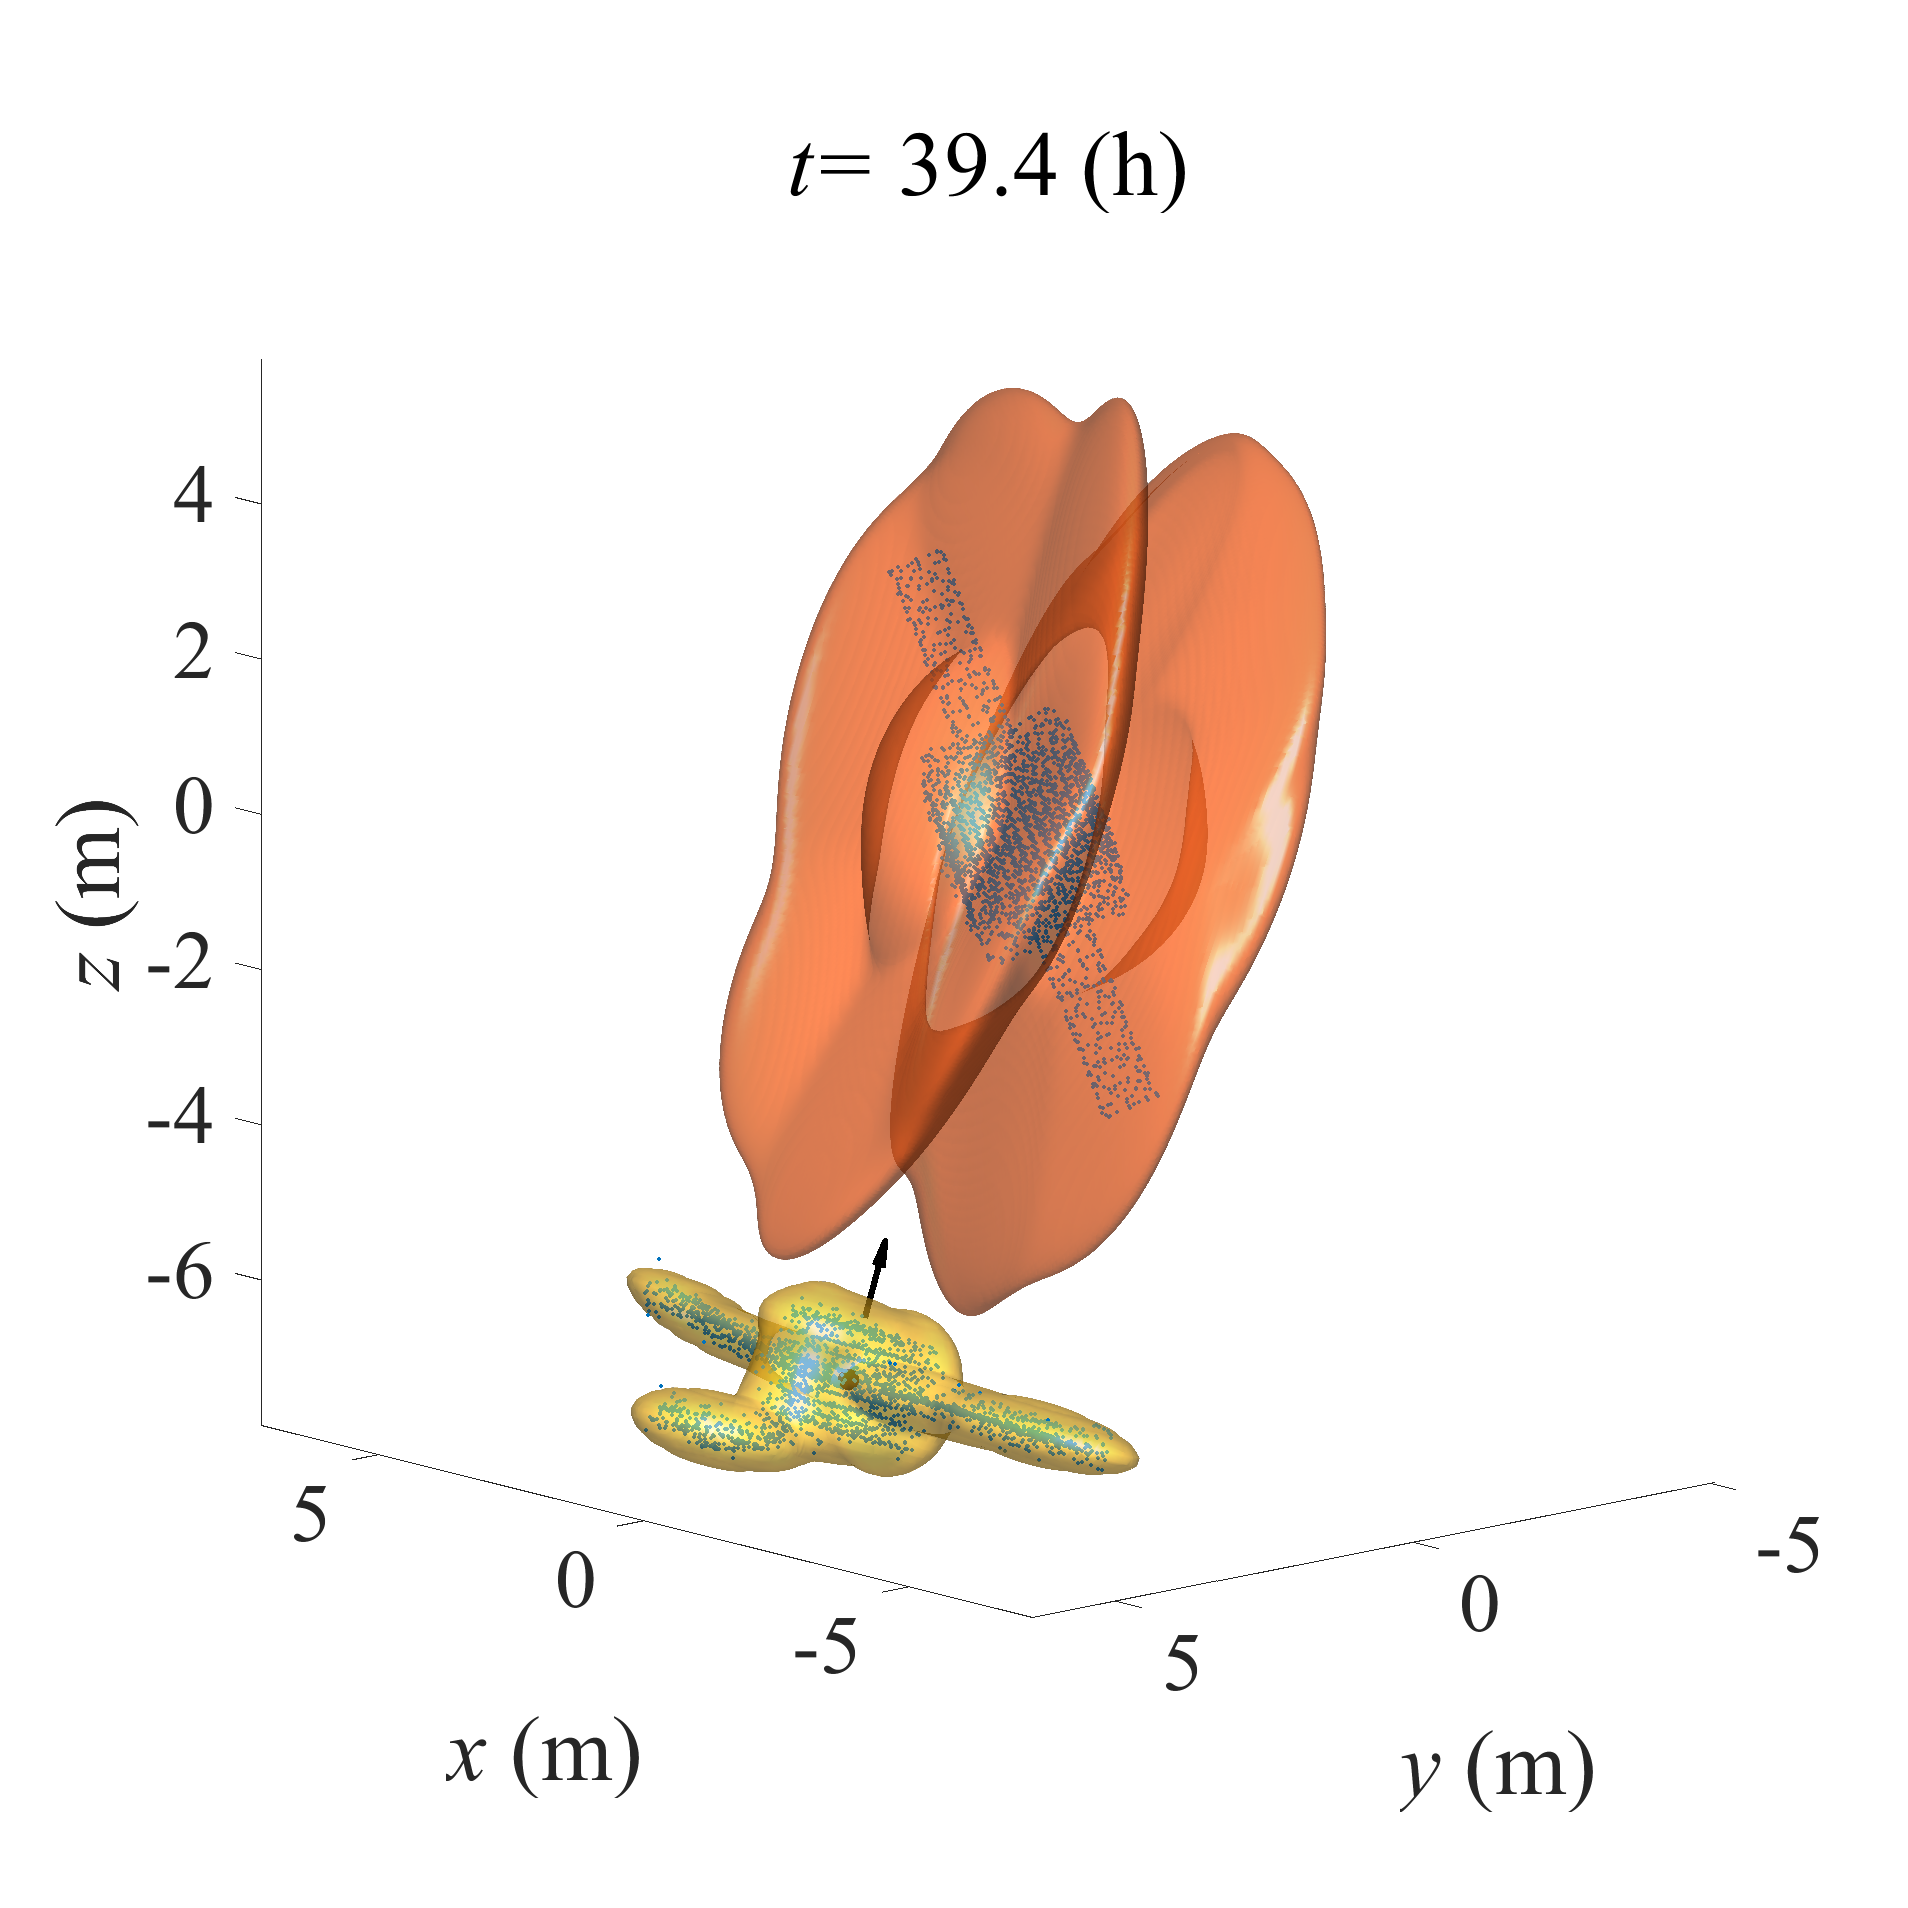
\includegraphics[width = 2.5in]{picture/posefix_detumble_time.eps}
			\caption{ }
			\label{fig:posefix_detumble_pose}
		\end{subfigure}\hfill
		\begin{subfigure}[t]{0.47\textwidth}
			\centering
			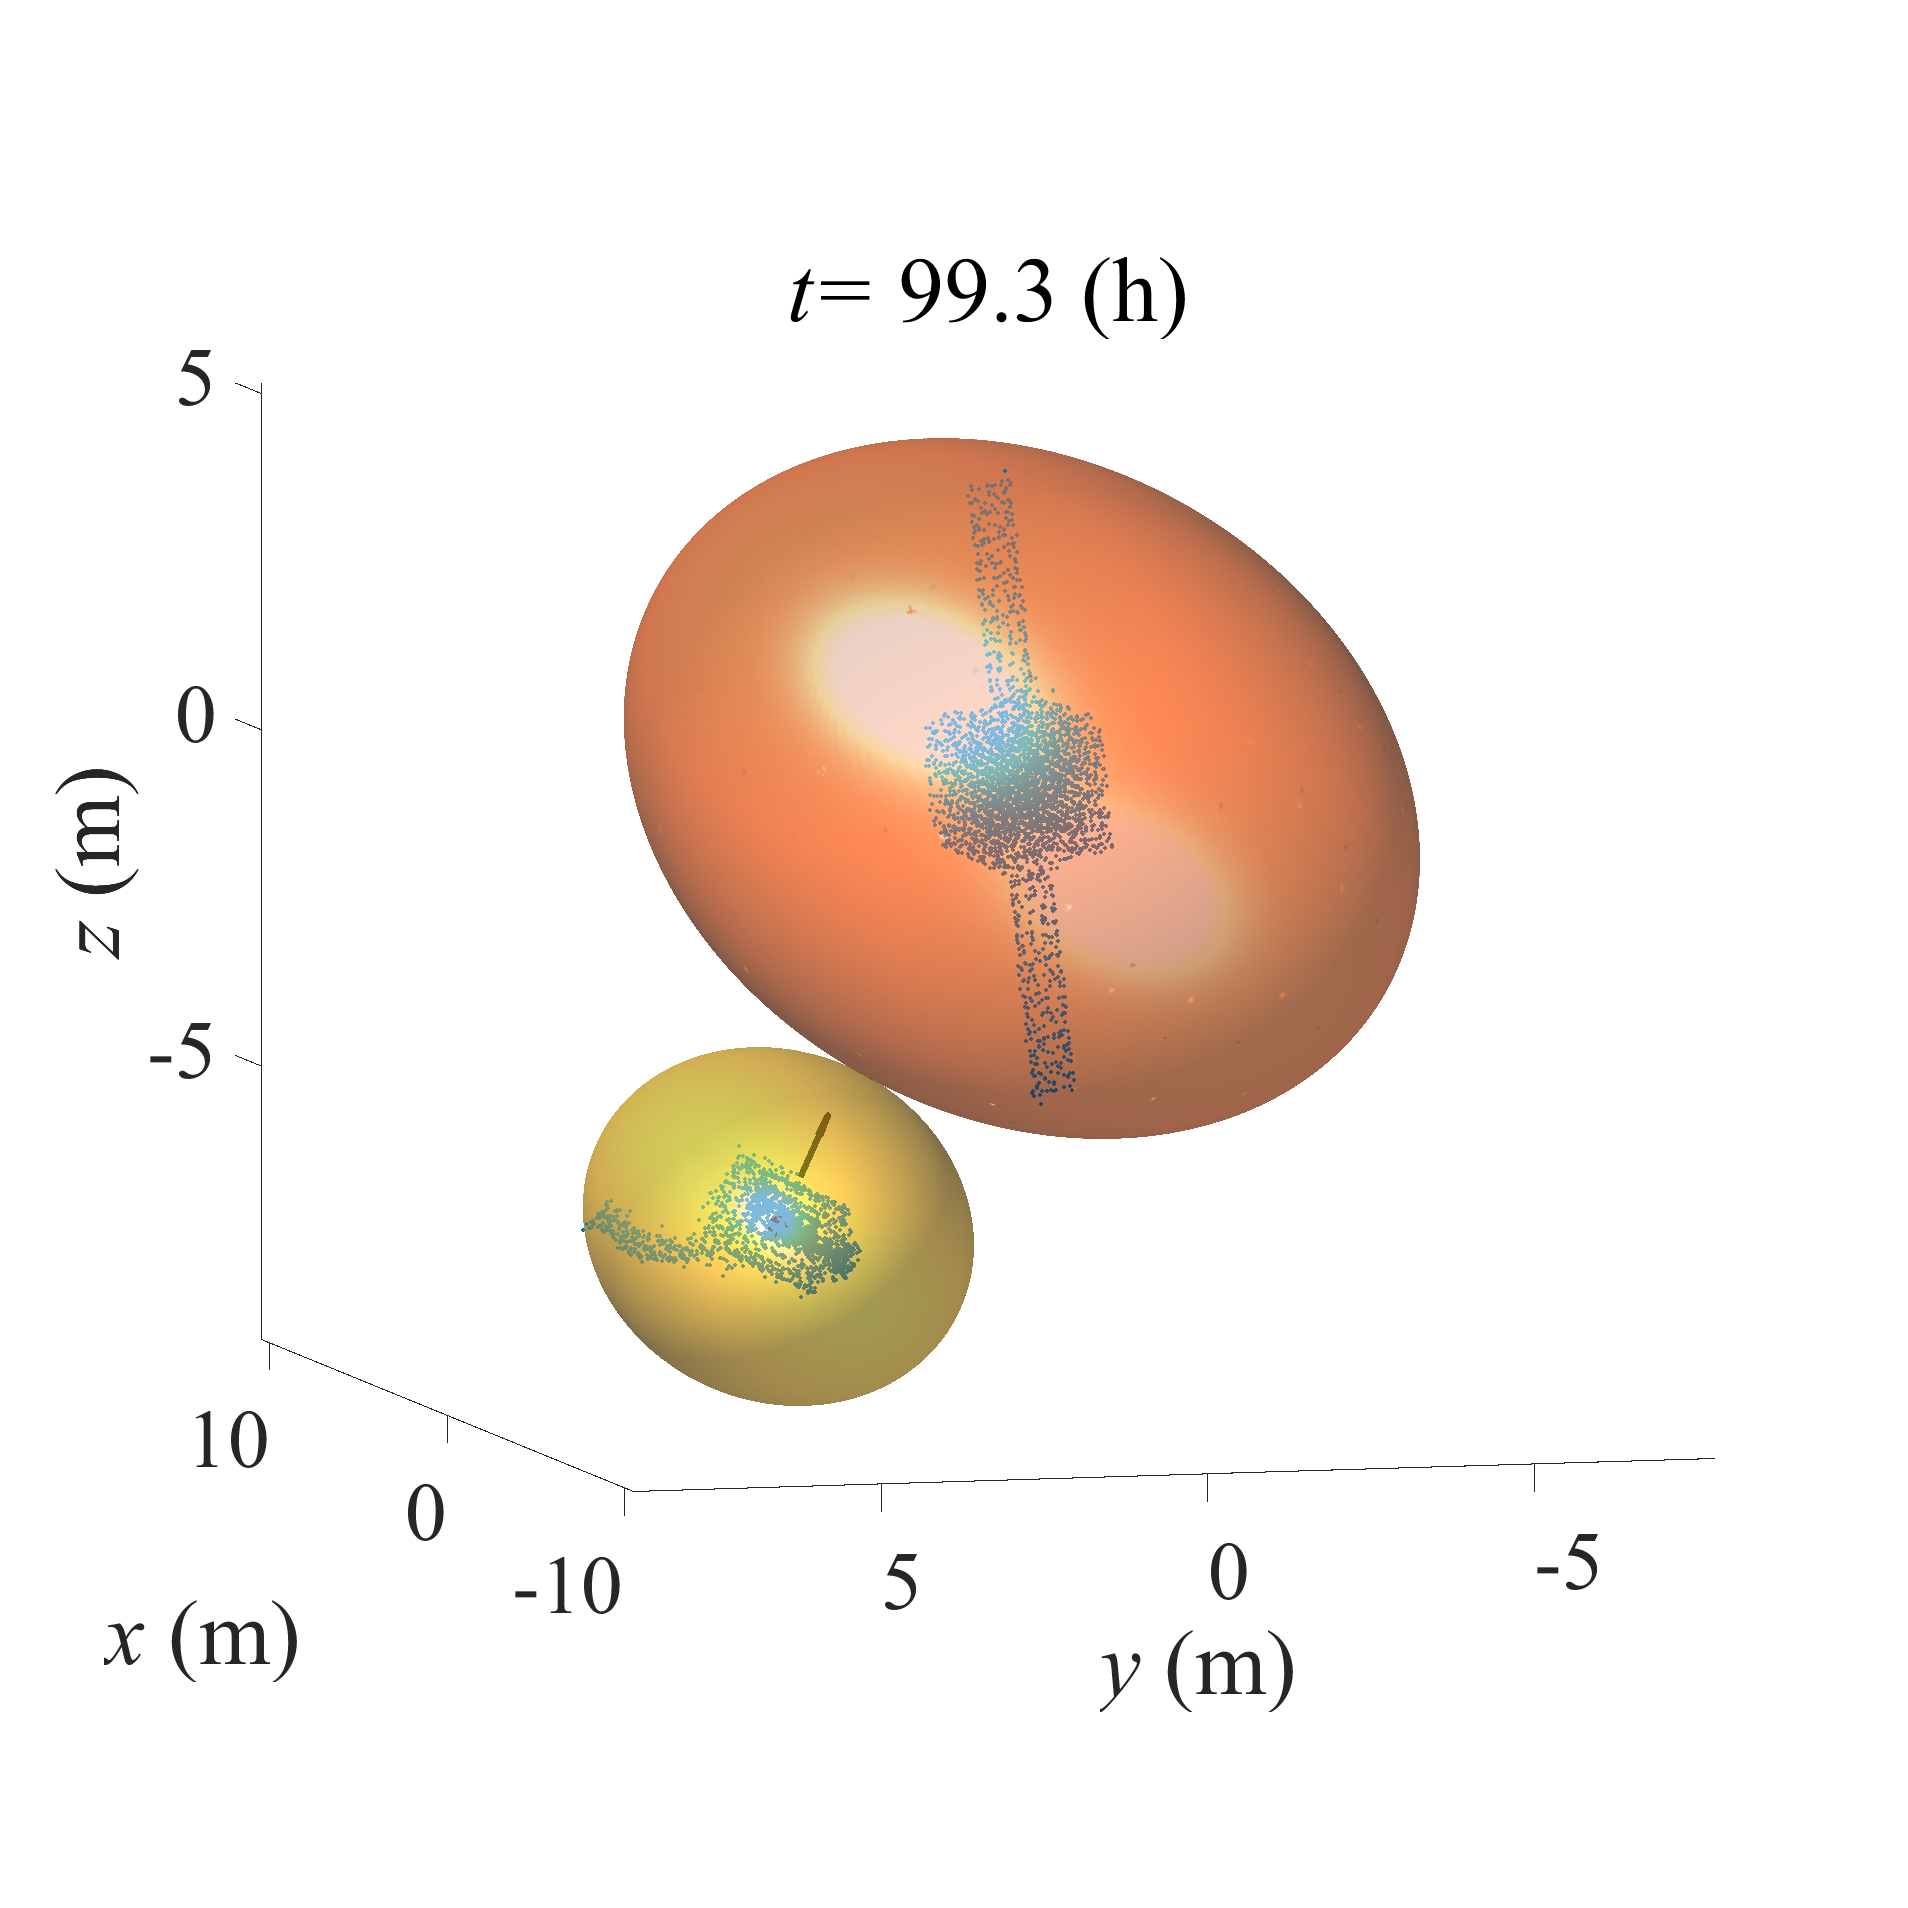
\includegraphics[width = 2.5in]{picture/fix_detumble_time.eps}
			\caption{ }
			\label{fig:fix_detumble_pose}
		\end{subfigure}
	\end{minipage}
	\caption{固定构型及固定位姿策略消旋过程中的相对位姿情况\label{Fig.posefix_detumble_pose}}
\end{figure*}

三种消旋策略的消旋效果如图\ref{Fig.posechangedetumb_time}、图\ref{Fig.posefixdetumb_time}和图\ref{Fig.fixdetumb_time}所示,对比各图可以看出,本文提出的切换构型消旋策略在平行构型效率较低时切换至垂直构型,保证消旋全过程均具有理想的消旋效率,总耗时$3.6\ (\mathrm{h})$。固定构型的消旋策略起始时刻消旋效率与本文方法一致,但随着目标章动角的增大,该构型下目标与服务星间的安全距离增大,目标质心处磁场强度迅速下降,导致消旋效率急剧降低,耗时$39.2\ (\mathrm{h})$将目标角速度降至容许范围。而采用椭球安全区域的固定位姿消旋策略,由于安全约束保守性较大,服务星所能产生的消旋力矩较小,消旋总耗时$101.4\ (\mathrm{h})$。因此相比现有方法,本文提出的消旋策略能在保证服务星安全的前提下显著提升电磁消旋的效率,有助于电磁消旋任务的具体实施。
\begin{figure*}[htb!]
	\centering
	\begin{minipage}[t]{0.96\textwidth}
		\centering
		\begin{subfigure}[t]{0.23\textwidth}
			\centering
			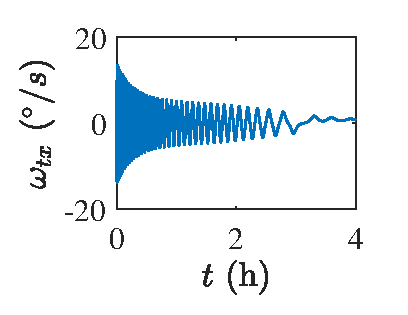
\includegraphics[width = 1.475in]{picture/posechange_omega_x.eps}
			\caption{ }
			\label{fig:posechangedetumb_time(a)}
		\end{subfigure}\hfill
		\begin{subfigure}[t]{0.23\textwidth}
			\centering
			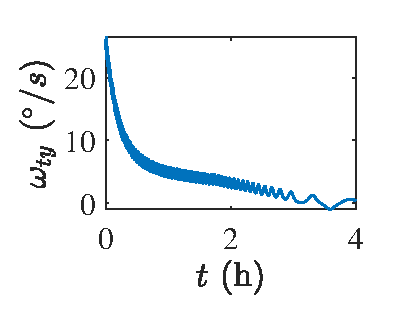
\includegraphics[width = 1.475in]{picture/posechange_omega_y.eps}
			\caption{ }
			\label{fig:posechangedetumb_time(c)}
		\end{subfigure}\hfill
		\begin{subfigure}[t]{0.23\textwidth}
			\centering
			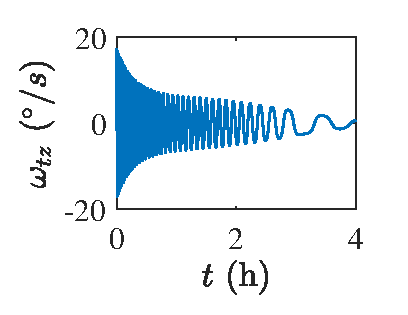
\includegraphics[width = 1.475in]{picture/posechange_omega_z.eps}
			\caption{ }
			\label{fig:posechangedetumb_time(e)}
		\end{subfigure}\hfill
		\begin{subfigure}[t]{0.23\textwidth}
			\centering
			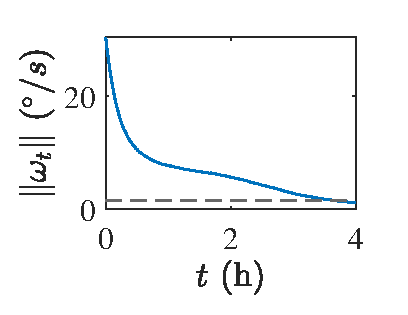
\includegraphics[width = 1.475in]{picture/posechange_omega_norm.eps}
			\caption{ }
			\label{fig:posechangedetumb_time(g)}
		\end{subfigure}
	\end{minipage}
	\caption{切换构型消旋耗时\label{Fig.posechangedetumb_time}}
\end{figure*}
\begin{figure*}[htb!]
	\centering
	\begin{minipage}[t]{0.96\textwidth}
		\centering
		\begin{subfigure}[t]{0.23\textwidth}
			\centering
			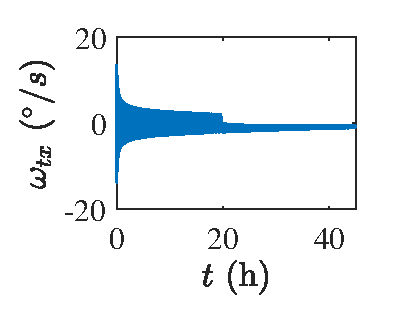
\includegraphics[width = 1.475in]{picture/posefix_omega_x.eps}
			\caption{ }
			\label{fig:posefixdetumb_time(a)}
		\end{subfigure}\hfill
		\begin{subfigure}[t]{0.23\textwidth}
			\centering
			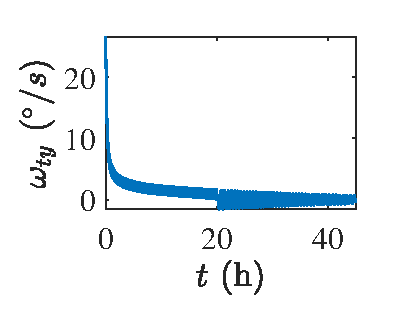
\includegraphics[width = 1.475in]{picture/posefix_omega_y.eps}
			\caption{ }
			\label{fig:posefixdetumb_time(c)}
		\end{subfigure}\hfill
		\begin{subfigure}[t]{0.23\textwidth}
			\centering
			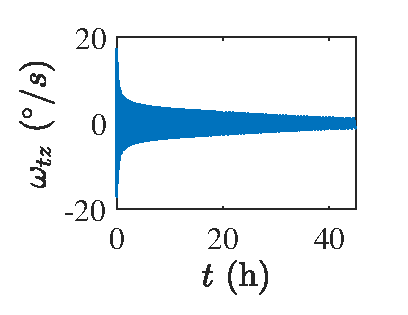
\includegraphics[width = 1.475in]{picture/posefix_omega_z.eps}
			\caption{ }
			\label{fig:posefixdetumb_time(e)}
		\end{subfigure}\hfill
		\begin{subfigure}[t]{0.23\textwidth}
			\centering
			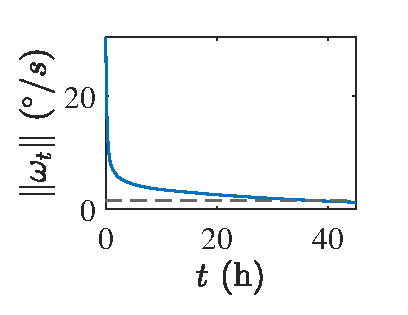
\includegraphics[width = 1.475in]{picture/posefix_omega_norm.eps}
			\caption{ }
			\label{fig:posefixdetumb_time(g)}
		\end{subfigure}
	\end{minipage}
	\caption{固定构型消旋耗时\label{Fig.posefixdetumb_time}}
\end{figure*}
\begin{figure*}[htb!]
	\centering
	\begin{minipage}[t]{0.96\textwidth}
		\centering
		\begin{subfigure}[t]{0.23\textwidth}
			\centering
			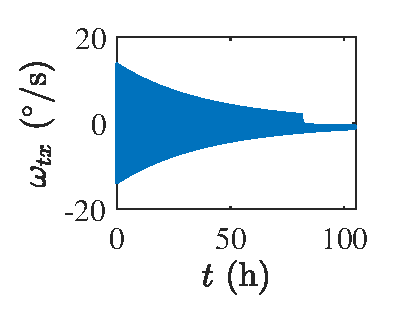
\includegraphics[width = 1.475in]{picture/fix_omega_x.eps}
			\caption{ }
			\label{fig:fixdetumb_time(a)}
		\end{subfigure}\hfill
		\begin{subfigure}[t]{0.23\textwidth}
			\centering
			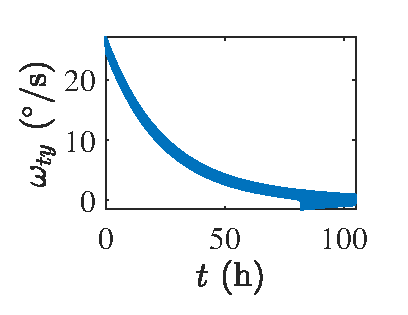
\includegraphics[width = 1.475in]{picture/fix_omega_y.eps}
			\caption{ }
			\label{fig:fixdetumb_time(c)}
		\end{subfigure}\hfill
		\begin{subfigure}[t]{0.23\textwidth}
			\centering
			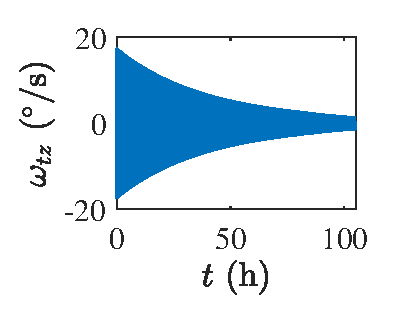
\includegraphics[width = 1.475in]{picture/fix_omega_z.eps}
			\caption{ }
			\label{fig:fixdetumb_time(e)}
		\end{subfigure}\hfill
		\begin{subfigure}[t]{0.23\textwidth}
			\centering
			\includegraphics[width = 1.475in]{picture/fix_omega_norm.eps}
			\caption{ }
			\label{fig:fixdetumb_time(g)}
		\end{subfigure}
	\end{minipage}
	\caption{固定位姿消旋耗时\label{Fig.fixdetumb_time}}
\end{figure*}

\section{本章小结}
本章针对复杂外形章动目标极近距离逼近与消旋过程中的位姿轨迹规划问题展开研究。两阶段均采用引导优化的规划框架,并根据二者对轨迹要求的不同对相关方法进行了调整。极近距离逼近阶段轨迹采用FMT*算法计算参考路径,随后对各控制点及轨迹时间进行优化,以给出满足各项约束的速度平滑位姿轨迹,有效减少了无效机动。极近距离消旋阶段为减少轨迹规划耗时,设计PPO算法以给出参考路径,随后对轨迹的控制点进行优化以满足碰撞约束并最大化消旋力矩,通过时间重分配算法保证轨迹速度、加速度可行,保证了消旋轨迹规划耗时满足要求,并极大提升了消旋效率。最后,进行了相关仿真验证,结果表明所提出的方法能在考虑章动目标、服务星复杂外形的前提下,给出安全无碰撞的可行位姿轨迹,实现章动目标的极近距离逼近,相比现有方法能有效减少电磁消旋所需时间。


\cleardoublepage

\chapter{物理引擎仿真与试验验证}
\chaptermark{物理引擎仿真与试验验证}
\section{引言}

%为验证所提出方法的可行性与有效性,本章对章动目标消旋地面实验系统进行了搭建。实验系统主要由目标章动旋转模拟装置、磁场源、机械臂和计算机组成,通过目标章动模拟装置模拟空间目标的章动旋转运动,通过机械臂抓取磁场源模拟服务星的运动。采用不同消旋轨迹进行了多组实验,记录目标角速度变化情况并对结果进行了比较分析。
为验证所提出方法的可行性与有效性,本章搭建了章动目标电磁消旋地面实验系统并进行了逼近消旋等实验。首先,本章描述了实验系统的整体架构,并对实验系统的软硬件设计进行了介绍;随后,为保证实验的顺利实施,对实验相关参数的确定进行了分析,并对仿真实验环境进行了介绍;最后,本章设计并进行了相关消旋实验,对实验数据进行了对比分析。

\section{消旋实验系统设计搭建}
本文中章动目标电磁消旋地面实验系统需实现的主要功能包括目标的章动旋转控制、目标角速度的准确测量、磁场源位置与姿态运动控制。为实现上述功能,本章搭建地面实验系统如图\ref{fig:exp_sys}所示,可分为启旋与测量模块、章动模拟模块和磁场源运动控制模块,主要包括目标章动旋转模拟装置、磁场源、Kuka机械臂、计算机等。通过目标章动模拟装置中的电机控制目标章动旋转,通过角速度传感器测量目标转速,通过机械臂抓取磁场源执行给定轨迹。下面对系统中涉及的软硬件进行介绍。
\begin{figure}[htbp]
	\centering
	\includegraphics[width = 5.4in]{picture/experiment_sys.png}
	\caption{电磁消旋实验系统组成}
	\label{fig:exp_sys}
\end{figure}

\subsection{目标章动旋转模拟装置设计}
目标章动旋转模拟装置结构如图\ref{Fig.tar_sys_all}所示,可分为上方的目标章动模拟模块和下方的启旋与测量模块。
\begin{figure*}[htbp]
	\centering
	\begin{minipage}[t]{0.96\textwidth}
		\centering
		\begin{subfigure}[t]{0.47\textwidth}
			\centering
			\includegraphics[width = 2.5in]{picture/target_sys_solidwork.png}
			\caption{ }
			\label{fig:tar_sys_solidwork}
		\end{subfigure}\hfill
		\begin{subfigure}[t]{0.47\textwidth}
			\centering
			\includegraphics[width = 2.5in]{picture/target_sys.pdf}
			\caption{ }
			\label{fig:tar_sys}
		\end{subfigure}
	\end{minipage}
	\caption{目标章动旋转模拟装置设计图\label{Fig.tar_sys_all}}
\end{figure*}

启旋与测量模块外部采用铝合金板支撑,保证结构刚度的同时避免被磁化影响实验效果。铝合金板两侧加工有螺纹孔,可横向安装铝合金板为所需设备提供支撑。该模块中所安装的设备包括转动电机、离合器、角速度传感器,通过离合器连接电机轴和主传动轴;转动电机带动目标章动模拟模块旋转;通过角速度传感器对目标章动模拟装置角速度进行高频测量。

章动模拟模块采用尼龙板支撑,并使用尼龙螺栓、螺母固定,避免模块旋转时外壳激发涡电流影响实验效果。章动模拟模块内部安装有锂电池、STM32控制板和章动控制电机,通过锂电池为STM32控制板和章动控制电机供电;STM32控制板向章动控制电机驱动器发送脉冲信号以控制电机转动;章动控制电机依次通过减速器、梅花联轴器、同步带、同步轮等结构与模拟目标连接,带动模拟目标旋转以改变其章动角。

模拟目标采用常见的立方星外形,加工材质为铝合金,主体为边长$25\ (\mathrm{cm})$,厚度$2\ (\mathrm{mm})$的立方壳,两侧安装有长$37.5\ (\mathrm{cm})$,宽$10\ (\mathrm{cm})$的模拟太阳帆板。目标总长为$1\ (\mathrm{m})$,质量为$2.73\ (\mathrm{kg})$,转动惯量为$\mathrm{diag}(0.0651,0.0448,0.069)\ (\mathrm{kg\cdot m^2})$。目标安装处通过亚克力板与其余部件绝缘隔离,避免目标表面涡电流外溢耗散,影响实验效果。

目标章动旋转模拟装置中的各传动轴均安装于陶瓷轴承中,从而减小摩擦阻力并保证其大小基本恒定,以便于对摩擦力矩进行拟合。

目标章动旋转模拟装置的工作流程为:闭合离合器,开启转动电机带动章动模拟模块旋转,通过角速度传感器测量目标角速度,到达指定转速后,断开离合器使章动模拟模块自由旋转,通过章动控制电机改变模拟目标章动角,记录角速度传感器所测得的目标角速度变化情况。本装置可模拟空间章动目标的两轴旋转,模拟目标的运动区域与本文所构建的角动量定向型安全区域基本吻合,可用于验证本文方法的有效性。装置中使用的主要设备的选型与参数介绍如下。

\subsubsection{转动电机选型}
装置中的章动模拟模块总重量为$6.6\ (\mathrm{kg})$,沿旋转轴方向转动惯量约为$0.191\ (\mathrm{kg\cdot m^2})$,综合考虑负载大小、电磁消旋效果、结构强度等因素,确定模拟目标的设计转速为$3.3\pi\ (\mathrm{rad/s})$,即$100\ (\mathrm{rpm})$。根据上述参数,选择无刷电机GM6020作为装置转动电机,如图\ref{fig:wushuamotor}所示,该电机使用磁场定向控制算法,可通过闭环速度控制精确调节电机转速,最大转速为$320\ (\mathrm{rpm})$,额定扭矩为$1.2\ (\mathrm{N \cdot m})$,额定转速下的调速范围为$0\sim 132\ (\mathrm{rpm})$,可以满足装置需求。
\begin{figure}[htbp]
	\centering
	\includegraphics[width = 2.5in]{picture/wushuamotor.jpg}
	\caption{无刷电机实物图}
	\label{fig:wushuamotor}
\end{figure}

\subsubsection{离合器选型}
章动模拟模块到达指定转速后需与转动电机轴分离,进入自由旋转状态,为尽可能减小自由旋转状态下章动模拟模块所受阻力,选择干式单片电磁离合器连接章动模拟模块与转动电机轴,其工作电压为$24$伏,通过串口继电器控制通断,最大转矩为$1.1\ (\mathrm{N \cdot m})$,如图\ref{fig:diancilihe}所示。所选电磁离合器主要由制动片、预压式弹片、电磁线圈等构成,接入直流电源后将产生磁场使制动片和弹片吸合,通过二者间的摩擦力传递扭矩,断开电流后制动片将与弹片分离,避免转动电机对章动模拟模块的自由转动产生干扰。
\begin{figure}[ht]
	\centering
	\includegraphics[width = 2.5in]{picture/diancilihe.jpg}
	\caption{电磁离合器实物图}
	\label{fig:diancilihe}
\end{figure}

\subsubsection{章动控制电机参数选型}
本装置中模拟目标章动旋转时,由于两侧帆板的质心高度不同,将产生回转力矩$T_{r}$,如图\ref{fig:huizhuan_tor}所示。立方壳体偏心距离较小,可忽略其影响,则$T_{r}$可由下式计算:
\begin{equation}
	\begin{aligned}
		\label{Tor_r}
		T_{r}&=2F_{r}l\sin(\theta)\\
		&=m_{p}\omega^{2}l^{2}\sin(2\theta)
	\end{aligned}
\end{equation}

\begin{figure}[htbp]
	\centering
	\includegraphics[width = 2.5 in]{picture/huizhuan_tor_pic.png}
	\caption{回转力矩示意图}
	\label{fig:huizhuan_tor}
\end{figure}
所使用的模拟帆板质量$m_{p}=0.18\ (\mathrm{kg})$,质心距转动中心距离$l=0.32\ (\mathrm{m})$,目标的设计转速为$3.3\pi\ (\mathrm{rad/s})$,根据\autoref{Tor_r},在$\theta=45\ (\mathrm{^\circ})$时回转力矩最大,$T_{r,\max}=1.98\ (\mathrm{N \cdot m})$。

为抵消目标回转力矩,实现目标章动角控制,选择带行星齿轮减速器的步进电机作为章动控制电机,如图\ref{Fig.stepmotor_reducer}所示。其中步进电机的额定转矩为$0.42\ (\mathrm{N \cdot m})$,行星齿轮减速器的减速比为$1:10$,装置中同步带轮的传动比为$1.43$,故该电机可提供$6.01\ (\mathrm{N \cdot m})$的保持力矩,能够满足装置需要。
\begin{figure*}[htbp]
	\centering
	\begin{minipage}[t]{0.96\textwidth}
		\begin{subfigure}[t]{0.47\textwidth}
			\centering
			\includegraphics[width = 2.5in]{picture/stepmotor.jpg}
			\caption{ }
			\label{fig:stepmotor}
		\end{subfigure}\hfill
		\begin{subfigure}[t]{0.47\textwidth}
			\centering
			\includegraphics[width = 2.5in]{picture/reducer2.jpg}
			\caption{ }
			\label{fig:reducer}
		\end{subfigure}
	\end{minipage}
	\caption{步进电机及减速器实物图\label{Fig.stepmotor_reducer}}
\end{figure*}

\subsubsection{角速度传感器选型}
为更好的验证电磁消旋效果,需对目标角速度进行高频、高精度的测量。常见的角速度传感器包括陀螺仪型角速度传感器、霍尔式编码器、电容式编码器和光电编码器等,其中陀螺仪型角速度传感器分辨率与测量频率较低,霍尔式编码器和电容式编码器易受电磁干扰,不适用于本实验,因此选择一体式增量光电编码器作为角速度传感器,如图\ref{Fig.anglecoder}所示。该编码器搭配2500线码盘,输出双相脉冲信号,经编码器采集卡处理后可获得角速度信息,最高分辨率为$0.036\ (\mathrm{^\circ})$,最高允许转速为$5000\ (\mathrm{rpm})$。
\begin{figure*}[htbp]
	\centering
	\begin{minipage}[t]{0.96\textwidth}
		\begin{subfigure}[t]{0.47\textwidth}
			\centering
			\includegraphics[width = 2.5in]{picture/anglecoder.png}
			\caption{ }
			\label{fig:anglecoder}
		\end{subfigure}\hfill
		\begin{subfigure}[t]{0.47\textwidth}
			\centering
			\includegraphics[width = 2.5in]{picture/anglecoder_pic.jpg}
			\caption{ }
			\label{fig:anglecoder_pic}
		\end{subfigure}
	\end{minipage}
	\caption{光电编码器结构图\label{Fig.anglecoder}}
\end{figure*}

\subsection{磁场源运动控制模块设计}
磁场源运动控制模块包括磁场源和机械臂系统,通过机械臂抓取永磁体执行逼近及消旋轨迹。为获得理想的消旋效果,磁场源应提供足够强度的磁场,装置中磁场源采用钕铁硼永磁体,牌号为N48,使用多片定制磁体组合而成,直径为$100\ (\mathrm{mm})$,总厚度为$50\ (\mathrm{mm})$,表面磁场强度可达$4200\ (\mathrm{Gs})$。磁体夹具使用PA10尼龙制作,如图\ref{Fig.sys_magnet}所示,二者总质量为$3.8\ (\mathrm{kg})$。
\begin{figure*}[htbp]
	\centering
	\begin{minipage}[t]{0.96\textwidth}
		\begin{subfigure}[t]{0.47\textwidth}
			\centering
			\includegraphics[width = 2.5in]{picture/magnet.jpg}
			\caption{ }
			\label{fig:magnet}
		\end{subfigure}\hfill
		\begin{subfigure}[t]{0.47\textwidth}
			\centering
			\includegraphics[width = 2.5in]{picture/magnet_holder.jpg}
			\caption{ }
			\label{fig:magnet_holder}
		\end{subfigure}
	\end{minipage}
	\caption{永磁体实物图\label{Fig.sys_magnet}}
\end{figure*}

机械臂采用Kuka iiwa 14 R820系统,其系统组成主要包括机械臂本体、控制柜与示教器,可通过计算机连接控制柜对机械臂进行离线编程,通过示教器完成程序的载入与运行,实现机械臂的在线控制。
%\begin{figure}[htbp]
%	\centering
%	\includegraphics[width = 3.55in]{picture/kuka.png}
%	\caption{Kuka iiwa机械臂}
%	\label{fig:robot_arm}
%\end{figure}

机械臂本体负载为$14\ (\mathrm{kg})$,臂展为$820\ (\mathrm{mm})$,具有七个可控关节,从底部到末端依次记为$A_{1}\sim A_{7}$,末端关节带有法兰盘,可连接各种负载。机械臂各关节速度、关节角范围限制如表\ref{Table_robot_arm}所示。
\begin{table}[!htb]
	\caption{机械臂关节参数限制范围}
	\label{Table_robot_arm}
	\centering
	
	\begin{tabularx}{\textwidth}{CCC}
		\toprule
		% after \\: \hline or \cline{col1-col2} \cline{col3-col4} ...
		关节 							      & 最高转速 					& 关节角范围 					  \\
		\midrule
		$A_{1}$ 	&	$85\ (\mathrm{^\circ/s})$	    	&	$-170\sim 170\ (\mathrm{^\circ})$		\\
		$A_{2}$ 	&	$85\ (\mathrm{^\circ/s})$	    	&	$-120\sim 120\ (\mathrm{^\circ})$		\\
		$A_{3}$ 	&	$100\ (\mathrm{^\circ/s})$	    	&	$-170\sim 170\ (\mathrm{^\circ})$			\\
		$A_{4}$ 	&	$75\ (\mathrm{^\circ/s})$	    	&	$-120\sim 120\ (\mathrm{^\circ})$			\\
		$A_{5}$ 	&	$130\ (\mathrm{^\circ/s})$	    	&	$-170\sim 170\ (\mathrm{^\circ})$	 \\
		$A_{6}$ 	&	$135\ (\mathrm{^\circ/s})$	    	&	$-120\sim 120\ (\mathrm{^\circ})$  \\
		$A_{7}$ 	&	$135\ (\mathrm{^\circ/s})$	    	&	$-175\sim 175\ (\mathrm{^\circ})$		\\
		\bottomrule
	\end{tabularx}
\end{table}

\subsection{软件系统设计}
为整合各设备,减少操作步骤,基于$C\#$开发章动目标模拟装置控制软件,软件与各设备间的通讯连接如图\ref{fig:software_connet}所示。
\begin{figure}[hbt]
	\centering
	\includegraphics[width = 3.55in]{picture/software_connet.png}
	\caption{章动目标模拟装置控制软件通讯连接图}
	\label{fig:software_connet}
\end{figure}

其中,软件与编码器采集卡间采用RS485通讯协议传递角速度信息,传输频率为$50\ (\mathrm{Hz})$。软件与无刷电机间采用CAN通讯,通讯周期为$10\ (\mathrm{ms})$,设定无刷电机速度后其内置的驱动器将对电机速度进行闭环控制。软件通过串口协议与串口继电器通讯,控制离合器通断。步进电机与STM32控制卡位于章动模拟模块中,需随模拟目标一起旋转,无法直接与计算机连接,若采用滑环连接则会引入较大的摩擦阻力,故软件与STM32控制板间采用蓝牙通讯,通过STM32控制板发送脉冲信号控制步进电机运动。
\begin{figure}[htb!]
	\centering
	\includegraphics[width = 5.4in]{picture/software_panel.png}
	\caption{章动目标模拟装置控制软件界面图}
	\label{fig:software_panel}
\end{figure}

软件具有角速度信息采集与显示、电磁离合器通断控制、无刷电机控制、步进电机控制、数据导出等功能,其界面如图\ref{fig:software_panel}所示。其工作流程为:选择对应串口连接各设备后,软件在界面下方实时绘制目标角速度变化曲线,通过对应按钮控制电磁离合器闭合,设定无刷电机速度,当光电编码器返回的目标角速度到达设定的期望值后,软件将控制电磁器断开,控制步进电机运动使模拟目标开始章动旋转,实验完成后,将目标角速度变化情况导出至Excle文件中。


\subsection{系统操控框架}
章动目标电磁消旋地面实验系统操控框架如图\ref{fig:sys_box}所示,完整实验流程为:计算机控制无刷电机通过电磁离合器带动章动模拟模块旋转,控制机械臂抓取永磁体执行逼近轨迹;通过编码器采集目标角速度,检测目标角速度到达指定值后,断开电磁离合器,通过步进电机改变模拟目标章动角,控制机械臂执行消旋轨迹,目标角速度降至$0\ (\mathrm{^\circ/s})$后,实验流程结束,记录目标角速度变化情况。
\begin{figure}[htbp]
	\centering
	\includegraphics[width = 5.4in]{picture/sys_box.png}
	\caption{系统操控框架图}
	\label{fig:sys_box}
\end{figure}


\section{仿真实验环境构建与验证}
本文所提出的轨迹规划方法适用对象为携带磁场源且可自由移动的服务星,与地面实验系统中使用机械臂控制磁场源运动有所不同,故所给出的轨迹仅为机械臂末端的轨迹。为保证实验的安全性,避免给出的轨迹超出机械臂工作范围或执行轨迹时机械臂其他关节与目标发生碰撞,在进行实际实验前,本章先构建了仿真实验环境以验证轨迹的可行性。

如前所述,将机械臂末端关节与磁体视为本文研究场景中的服务星,根据定义建立对应坐标系并通过所提出的GMMCRA法分别构建地面实验系统中的模拟目标和服务星的安全区域如图\ref{fig:sys_safezone}所示,其中$\mathcal{A} = \{ {O_\mathcal{A}},{{\boldsymbol{\hat a}}_x},{{\boldsymbol{\hat a}}_y},{{\boldsymbol{\hat a}}_z}\} $为机械臂基座坐标系。
\begin{figure}[htbp]
	\centering
	\includegraphics[width = 3.55in]{picture/sys_safezone.png}
	\caption{地面实验系统模拟目标与服务星安全区域}
	\label{fig:sys_safezone}
\end{figure}

为避免装置发生干涉,实验中目标最大章动角设定为$45\ (\mathrm{^\circ})$,消旋过程中缓慢变为$90\ (\mathrm{^\circ})$,该方向的角速度极小可以忽略,即认为目标角速度始终沿转动电机轴方向,且目标质心位置恒定,故不同章动角下服务星的最优消旋位姿和消旋轨迹可以预先计算。服务星起始相对位姿设定为${{\boldsymbol{x}}_\mathcal{B}^{\mathcal{L}}}(0)=[0.618,0,0.684]^{\top}\ (\mathrm{m})$和${{\boldsymbol{\varphi}}_\mathcal{B}^{\mathcal{L}}}(0)=[\pi/2,\pi/2,\pi/2]^{\top}\ (\mathrm{rad})$,通过所提出的轨迹规划方法给出逼近及消旋切换轨迹如图\ref{Fig.exp_tra}所示。
\begin{figure*}[htbp]
	\centering
	\begin{minipage}[t]{0.96\textwidth}
		\begin{subfigure}[t]{0.47\textwidth}
			\centering
			\includegraphics[width = 2.5in]{picture/exp_proximity_tra.eps}
			\caption{ }
			\label{fig:exp_proximity_tra}
		\end{subfigure}
		\begin{subfigure}[t]{0.47\textwidth}
			\centering
			\includegraphics[width = 2.5in]{picture/exp_detumble_tra.eps}
			\caption{ }
			\label{fig:exp_detumble_tra}
		\end{subfigure}
	\end{minipage}
	\caption{地面实验逼近与消旋轨迹\label{Fig.exp_tra}}
\end{figure*}

考虑到机械臂工作空间有限,为确保轨迹可执行,同时避免章动目标与机械臂碰撞,需确定一合适的相对距离${{\boldsymbol{x}}_\mathcal{L}^{\mathcal{A}}}$,使得服务星轨迹始终在机械臂工作空间内,且机械臂执行轨迹时不与章动目标发生碰撞。通过机械臂正向运动学给出机械臂基座坐标系下的末端工作空间,根据待执行轨迹与模拟目标尺寸确定目标与机械臂底座间的距离为${{\boldsymbol{x}}_\mathcal{L}^{\mathcal{A}}}=[0.562,0,-0.75]^{\top}\ (\mathrm{m})$,如图\ref{Fig.arm_workplace}所示,其中橙黄色曲面表示机械臂的末端工作空间,紫色曲线为机械臂末端轨迹。
\begin{figure*}[htbp]
	\centering
	\begin{minipage}[t]{0.96\textwidth}
		\begin{subfigure}[t]{0.47\textwidth}
			\centering
			\includegraphics[width = 2.5in]{picture/workplace1.eps}
			\caption{ }
			\label{fig:workplace1}
		\end{subfigure}\hfill
		\begin{subfigure}[t]{0.47\textwidth}
			\centering
			\includegraphics[width = 2.5in]{picture/workplace2.eps}
			\caption{ }
			\label{fig:workplace2}
		\end{subfigure}
	\end{minipage}
	\caption{机械臂工作空间计算\label{Fig.arm_workplace}}
\end{figure*}

给定${{\boldsymbol{x}}_\mathcal{L}^{\mathcal{A}}}$后,通过坐标变换将逼近及消旋轨迹转化为机械臂基座坐标系下的末端位姿轨迹。由于iiwa 14机械臂存在冗余自由度,无法直接根据末端位姿确定唯一的关节配置,采用文献\oldcite{7dofarm}中的方法,固定臂形角为$0\ (\mathrm{^\circ})$,则通过逆运动学可得末端轨迹对应的机械臂关节角。机械臂关节角及其转速变化如图\ref{fig:arm_angle}所示,可以看出,机械臂各关节角及其转速满足表\ref{Table_robot_arm}中的参数限制,可通过机械臂抓取服务星执行逼近及消旋轨迹。
\begin{figure}[htbp]
	\centering
	\includegraphics[width = 3.55in]{picture/arm_angle.eps}
	\caption{切换构型策略中机械臂关节角与关节转速变化}
	\label{fig:arm_angle}
\end{figure}


类似的,给出固定构型和固定位姿消旋策略进行对比,其中固定构型的消旋策略仍采用GMMCRA法确定安全位姿,固定位姿的消旋策略采用椭球形安全区域,所使用的目标椭球安全区域参数为${\boldsymbol{E}}{{\boldsymbol{s}}} = \mathrm{diag}({0.58^2},{0.54^2},{0.54^2})\ (\mathrm{m})$。固定构型和固定位姿策略下相对位姿示意图如图\ref{Fig.pose_posifix}所示。
\begin{figure*}[htbp]
	\centering
	\begin{minipage}[t]{0.96\textwidth}
		\begin{subfigure}[t]{0.47\textwidth}
			\centering
			\includegraphics[width = 2.5in]{picture/posefix.eps}
			\caption{ }
			\label{fig:posefix}
		\end{subfigure}\hfill
		\begin{subfigure}[t]{0.47\textwidth}
			\centering
			\includegraphics[width = 2.5in]{picture/posifix.eps}
			\caption{ }
			\label{fig:posifix}
		\end{subfigure}
	\end{minipage}
	\caption{固定构型及固定位姿消旋策略实验仿真示意图\label{Fig.pose_posifix}}
\end{figure*}


固定构型消旋策略中机械臂关节角变化如图\ref{fig:arm_angle_posefix}所示,固定位姿消旋策略中机械臂关节角从$A_{1}$至$A_{7}$依次为$[91.8,13.6,0,-107.4,-72.2,116.9,0]\ (^\circ)$,均满足参数限制。
\begin{figure}[htbp]
	\centering
	\includegraphics[width = 3.55in]{picture/arm_angle_posefix.eps}
	\caption{固定构型策略中机械臂关节角与关节转速变化}
	\label{fig:arm_angle_posefix}
\end{figure}

\section{电磁消旋实验设计与结果分析}
完成章动目标电磁消旋地面系统搭建与仿真实验验证后,本节对章动旋转目标开展逼近与消旋实验并与其它方法进行对比以验证本文方法的可行性与有效性,包括切换构型消旋实验、固定构型消旋实验、固定位姿消旋实验和空白对照实验,各实验的流程与结果介绍如下。

\subsection{切换构型消旋实验}
将目标初始章动角设为$45\ (^\circ)$,通过无刷电机驱动模拟目标旋转至$3.3\pi\ \rm{(rad/s)}$,机械臂抓取永磁体执行逼近轨迹,到达当前最优消旋位姿后,断开电磁离合器,模拟目标开始自由旋转,消旋过程中目标章动角以$0.5\ \rm{(^\circ/s)}$的速率增大,机械臂根据目标章动角的变化执行消旋轨迹以切换至新的最优消旋位姿,直至目标角速度降至$0\ (\mathrm{^\circ/s})$,实验过程中机械臂与目标的状态变化如图\ref{fig:change_exp}所示。
\begin{figure}[htbp]
	\centering
	\includegraphics[width = 5.4in]{picture/change_exp.png}
	\caption{切换构型消旋实验场景}
	\label{fig:change_exp}
\end{figure}

第0秒时永磁体处于设定的初始位置,随后机械臂抓取永磁体执行逼近轨迹,第20秒到达当前最优消旋位姿,开始对目标进行消旋;第20秒到第61秒磁体处于平行构型下,根据目标章动角变化调整自身位姿;第61秒时最优消旋位姿变为垂直构型,机械臂抓取永磁体执行消旋切换轨迹,第92秒到达新的最优消旋位姿;第92秒至191秒磁体处于垂直构型下,根据目标章动角变化调整自身位姿,直至目标角速度降为$0\ \rm{(^\circ/s)}$。

\begin{figure*}[htb]
	\centering
	\begin{minipage}[t]{0.96\textwidth}
		\centering
		\begin{subfigure}[t]{0.47\textwidth}
			\centering
			\includegraphics[width = 2.5in]{picture/changepose_errbar.eps}
			\caption{ }
			\label{fig:changepose_errbar}
		\end{subfigure}\hfill
		\begin{subfigure}[t]{0.47\textwidth}
			\centering
			\includegraphics[width = 2.5in]{picture/changepose_boxline.eps}
			\caption{ }
			\label{fig:changepose_boxline}
		\end{subfigure}
	\end{minipage}
	\caption{切换构型消旋实验结果\label{Fig.changepose_result}}
\end{figure*}

为提高实验的可靠性,进行了数次重复实验,通过光电编码器记录目标角速度变化,根据重复实验结果对消旋时间的标准差进行计算,其误差带图如图\ref{Fig.changepose_result}所示。从图中可知,切换构型消旋实验中,平均消旋时间为$170.8\ \rm{(s)}$,多次实验的消旋时间差异约为$3\ \rm{(s)}$,实验结果具有较好的稳定性。产生波动的主要原因是实验中机械臂抓取永磁体跟踪最优消旋位姿时存在一定偏差,同时装置中的章动旋转模块存在一定偏心,每次实验中轴承摩擦力存在微小差异,使得最终消旋时间存在一定波动。


\subsection{固定构型消旋实验}
固定构型消旋实验中设定目标转速为$3.3\pi\ \rm{(rad/s)}$,章动角以$0.5\ \rm{(^\circ/s)}$的速率增大,采用所提出的GMMCRA法确定安全位姿,与切换构型消旋实验一致。但此实验中永磁体始终位于平行构型,目标章动角变化时,仅改变永磁体与目标间的相对距离以避免发生碰撞,实验过程中机械臂与目标的状态变化如图\ref{fig:posefix_exp}所示。
\begin{figure}[htbp]
	\centering
	\includegraphics[width = 5.4in]{picture/posefix_exp.png}
	\caption{固定构型消旋实验场景}
	\label{fig:posefix_exp}
\end{figure}

第0秒到第20秒机械臂抓取永磁体逼近目标到达最优消旋位置,开始对目标进行消旋;第20秒到第214秒间永磁体始终位于平行构型下,随目标章动角变化调整自身位姿,直至消旋过程结束。

类似的,进行了多次重复实验,消旋时间误差带如图\ref{Fig.posefix_result}所示,平均消旋时间为$193.7\ \rm{(s)}$。
\begin{figure*}[htbp]
	\centering
	\begin{minipage}[t]{0.96\textwidth}
		\begin{subfigure}[t]{0.47\textwidth}
			\centering
			\includegraphics[width = 2.5in]{picture/posefix_errbar.eps}
			\caption{ }
			\label{fig:posefix_errbar}
		\end{subfigure}\hfill
		\begin{subfigure}[t]{0.47\textwidth}
			\centering
			\includegraphics[width = 2.5in]{picture/posefix_boxline.eps}
			\caption{ }
			\label{fig:posefix_boxline}
		\end{subfigure}
	\end{minipage}
	\caption{固定构型消旋实验结果\label{Fig.posefix_result}}
\end{figure*}

\subsection{固定位姿消旋实验}
固定位姿消旋实验中模拟目标转速设定为$3.3\pi\ \rm{(rad/s)}$,章动角以$0.5\ \rm{(^\circ/s)}$的速率增大,与固定构型消旋实验一致,但此实验采用椭球形安全区域,章动目标始终位于椭球形安全区域中,因此实验中机械臂不需要移动,永磁体与目标间的相对位置和姿态保持不变,实验过程如图\ref{fig:posifix_exp}所示。

\begin{figure}[htbp]
	\centering
	\includegraphics[width = 5.4in]{picture/posifix_exp.png}
	\caption{固定位姿消旋实验场景}
	\label{fig:posifix_exp}
\end{figure}

进行了多次重复实验,并对消旋时间误差带进行计算,固定位姿消旋实验中消旋时间误差带如图\ref{Fig.posifix_result}所示,平均消旋时间为$207.4\ \rm{(s)}$。
\begin{figure*}[htb]
	\centering
	\begin{minipage}[t]{0.96\textwidth}
		\centering
		\begin{subfigure}[t]{0.47\textwidth}
			\centering
			\includegraphics[width = 2.5in]{picture/posifix_errbar.eps}
			\caption{ }
			\label{fig:posifix_errbar}
		\end{subfigure}\hfill
		\begin{subfigure}[t]{0.47\textwidth}
			\centering
			\includegraphics[width = 2.5in]{picture/posifix_boxline.eps}
			\caption{ }
			\label{fig:posifix_boxline}
		\end{subfigure}
	\end{minipage}
	\caption{固定位姿消旋实验结果\label{Fig.posifix_result}}
\end{figure*}

\subsection{空白对照实验}
地面实验中立方形目标转动时具有较大的空气阻力,为排除空气阻力和轴承等部件间的摩擦力对实验结果的影响,以更好的比较不同消旋策略的效果,对不施加磁场情况下章动目标的自由旋转时间进行了测试,实验中模拟目标的初始转速仍设定为$3.3\pi\ \rm{(rad/s)}$,章动角以$0.5\ \rm{(^\circ/s)}$的速率增大,与上述实验保持一致,实验过程如图\ref{fig:freerota_exp}所示。
\begin{figure}[htb]
	\centering
	\includegraphics[width = 5.4in]{picture/freerota_exp.png}
	\caption{自由旋转实验场景}
	\label{fig:freerota_exp}
\end{figure}

\begin{figure*}[htb!]
	\centering
	\begin{minipage}[t]{0.96\textwidth}
		\begin{subfigure}[t]{0.47\textwidth}
			\centering
			\includegraphics[width = 2.5in]{picture/free_errbar.eps}
			\caption{ }
			\label{fig:free_errbar}
		\end{subfigure}\hfill
		\begin{subfigure}[t]{0.47\textwidth}
			\centering
			\includegraphics[width = 2.5in]{picture/free_boxline.eps}
			\caption{ }
			\label{free_boxline}
		\end{subfigure}
	\end{minipage}
	\caption{空白对照实验结果\label{Fig.free_result}}
\end{figure*}

多次重复得空白对照实验中目标角速度变化情况如图\ref{Fig.free_result}所示,模拟目标平均自转时间为$220.6\ \rm{(s)}$。



\subsection{实验结果对比与分析}
不同消旋策略下目标角速度变化对比如图\ref{fig:detumtime_compare}所示,从图中可以看出,由于固定位姿消旋策略采用了较为保守的椭球形安全区域,永磁体距章动目标较远,能产生的消旋力矩很小,目标角速度变化曲线几乎与自由旋转实验的角速度曲线重合。固定构型消旋策略采用本文所提出的基于混合高斯模型的安全区域,在目标章动角较大时,对应的最优消旋位姿与切换构型消旋策略的一致,图中两种策略的前半段角速度变化曲线基本重合。当目标章动角继续变小时,切换构型的消旋策略机动至新的构型,机动过程中消旋力矩略小于固定构型消旋策略,到达新的构型后目标角速度下降速度明显高于固定构型的消旋策略,与理论分析一致。
\begin{figure}[htb!]
	\centering
	\includegraphics[width = 3.55in]{picture/detumtime_compare.eps}
	\caption{不同实验中目标角速度变化}
	\label{fig:detumtime_compare}
\end{figure}

为获得无阻力干扰情况下的消旋时间,对目标角速度曲线进行差分得不同实验中目标所受外力矩。实验中目标所受外力矩主要包括目标转动受到的空气阻力矩、电磁消旋力矩和轴承产生的摩擦力矩。其中,空气阻力矩与角速度的平方成正比,电磁力矩与角速度成正比,所使用陶瓷轴承的摩擦力距基本为常数,故以目标角速度为自变量,采用二次函数对实验外力矩进行拟合,结果如图\ref{fig:exp_tor}所示。其中,切换构型实验中由于永磁体相对构型发生变化,前后力矩有明显变化,对其进行了分段拟合。
\begin{figure}[htb!]
	\centering
	\includegraphics[width = 3.55in]{picture/exp_tor.eps}
	\caption{不同实验中目标所受外力矩拟合曲线}
	\label{fig:exp_tor}
\end{figure}

获得各实验中力矩变化情况后,将各消旋实验中的目标所受外力矩减去自由旋转实验中外力矩,即可获得不同消旋实验中电磁消旋力矩随目标角速度的变化情况。设定计算步长为$0.1\ \rm{(s)}$,目标初始角速度为$3.3\pi\ \rm{(rad/s)}$,角速度降至$1.5\ \rm{(^\circ/s)}$时完成消旋,无空气阻力和摩擦力矩时不同消旋策略的消旋耗时如图\ref{fig:exp_simu_detum_time}所示。由图可知,切换构型消旋策略耗时$1374\ \rm{(s)}$,固定构型消旋策略起始时刻消旋效率与切换构型消旋策略一致,但当目标章动角增大时,该构型下安全距离增大,导致消旋效率急剧下降,总耗时$6803\ \rm{(s)}$;固定位姿消旋策略由于距离较远,能产生的消旋力矩较小,消旋耗时$17710\ \rm{(s)}$。各消旋策略的消旋耗时与第四章的消旋仿真结果基本吻合,表明相比传统的电磁消旋方法,基于本文方法的切换构型消旋策略能有效缩短消旋时间,提高电磁消旋效率,有助于空间电磁消旋的实际应用。
\begin{figure}[htb!]
	\centering
	\includegraphics[width = 3.55in]{picture/exp_simu_detum_time.eps}
	\caption{各消旋策略理想条件下消旋耗时}
	\label{fig:exp_simu_detum_time}
\end{figure}

\subsection{实验环境与空间环境差异分析}
由于地面实验环境与实际空间环境不同,章动目标电磁消旋地面实验系统中目标的尺寸、所受外部干扰、服务星的运动方式等与空间真实情况间存在一定差异,对其分析讨论如下:

\begin{enumerate}
	
	\item 受磁场源、机械臂等设备的尺寸限制,地面实验系统中的模拟目标为实际空间目标的缩比模型,其材质为铝合金,电导率与空间目标基本一致,地面实验中空气的相对磁导率近似为1,即与空间环境基本一致。若地面实验结果能够验证电磁涡流消旋的有效性,则说明电涡流法能对空间旋转目标进行消旋。
	
	\item 地面实验中模拟目标无最小惯量轴方向的转动,角动量轴固定,与空间目标章动运动存在一定差异。但本文方法确定的最优消旋位姿对空间章动目标施加的消旋力矩始终平行于目标角动量轴,由仿真结果可知,章动目标消旋过程中角动量轴方向基本恒定。同时,地面实验系统通过电机改变模拟目标章动角,使得模拟目标安全区域与空间章动目标基本一致,地面实验中服务星需执行的极近距离逼近与消旋轨迹与空间电磁消旋场景中基本一致,对极近距离消旋任务的实施有一定的参考意义。
	
	\item 与空间环境不同,地面实验中旋转的模拟目标将受到轴承的摩擦阻力与空气阻力,模拟目标的角速度将逐渐减小。因此地面实验中设置了模拟目标自由旋转的对照组实验,用于估计模拟目标转动过程中所受的阻力大小,进而获得地面实验中模拟目标所受的电磁消旋力矩大小,以验证本文方法的有效性,并对空间电磁消旋任务的耗时进行估计。
	
	\item 地面实验中采用七自由度机械臂抓取磁场源以模拟服务星的运动,本文中假定空间中的服务星采用连续动力推进,故地面实验中轨迹可行即可保证轨迹的连续性、平滑度满足要求,但空间环境中服务星动力学、最大驱动力与地面实验中不同,需调整服务星的速度、加速度限制使本文规划方法给出的轨迹满足服务星驱动力限制。

\end{enumerate}


\section{本章小结}
%为验证所提出方法的可行性与有效性,本章对章动目标消旋地面实验系统进行了搭建。实验系统主要由目标章动旋转模拟装置、磁场源、机械臂和计算机组成,通过目标章动模拟装置模拟空间目标的章动旋转运动,通过机械臂抓取磁场源模拟服务星的运动。采用不同消旋轨迹进行了多组实验,记录目标角速度变化情况并对结果进行了比较分析。
基于前文提出的章动目标极近距离逼近与消旋策略,本章对章动目标电磁消旋地面实验系统进行了设计,对系统中各设备进行了选型分析,并对系统软硬件进行了整合搭建,实现了空间章动目标的两轴转动模拟以及磁场源的位姿控制。根据实验中的模拟目标与磁场源的尺寸,基于第三章提出的GMMCRA法构建了安全区域与避撞约束,并根据第四章提出的极近距离逼近与消旋轨迹规划方法给出了磁场源的运动轨迹。将磁场源位姿轨迹转化为机械臂关节角,并在仿真环境中验证了机械臂轨迹的安全性和可行性后,本章开展了不同消旋策略下的电磁消旋实验,实验结果表明,基于GMMCRA法的安全约束有效可行,且精度相比传统约束有明显提高,为复杂外形目标的极近距离逼近奠定了基础;所提出的极近距离逼近与消旋轨迹规划方法能给出安全可行的位姿轨迹,且消旋效率相比传统方法大幅提升。

\cleardoublepage

\chapter{总结与展望}
\chaptermark{总结与展望}
空间章动目标消旋操控是大型非合作目标维修、回收或离轨等操作的必要前序步骤,其中电磁涡流消旋具有非接触、无额外工质消耗、适用性强等优势,受到广泛关注,极具发展与应用潜力。本文面向空间章动目标电磁消旋场景,主要研究任意形状目标间的碰撞风险分析问题、复杂章动目标极近距离逼近与消旋轨迹规划问题,并搭建地面实验系统以验证相关模型方法,全文工作总结如下:

\section{本文工作总结}
\begin{enumerate}
	\item 描述了空间目标电磁消旋任务场景与涉及的坐标系定义,针对电磁消旋场景中的相互机理,基于磁张量理论,给出了任意外形目标在非均匀磁场下所受电磁力和力矩的机理模型;在此基础上建立了惯性系下服务星与目标间的相对位置动力学方程和各自的姿态动力学方程。随后对相关概念进行了介绍,给出了本文中最优消旋位姿与位姿同步规划问题的定义。
	
	\item 针对任意外形航天器间的碰撞风险评估问题,在目标与服务星点云均已获得的前提下,通过混合高斯模型获得航天器外形的拓扑化描述,并在此基础上给出了精确安全区域的构建方法。对于章动旋转目标,根据其运动特点设计了角动量定向安全区域,避免了体固连安全区域的时变问题。随后,提出了基于混合高斯模型的碰撞危险度定义与其解析计算式,以评估航天器间的碰撞风险,并对碰撞危险度阈值的确定进行了分析,获得了两任意外形航天器间的准确碰撞约束。仿真分析表明所提出的GMMCRA法能对复杂外形航天器间的碰撞风险进行准确评估,求解迅速且精度明显高于传统的椭球安全区域。
	
	\item 针对复杂外形章动目标极近距离逼近与消旋过程中的位姿轨迹规划问题,基于引导优化的规划框架,通过B样条曲线构造轨迹,根据任务中极近距离逼近和极近距离消旋过程中对服务星轨迹的不同需求,结合GMMCRA法分别对其进行了设计。极近距离逼近阶段采用FMT*算法给出渐近最优的服务星逼近位姿参考路径,并设计优化问题对曲线的控制点和时间间隔进行优化,给出满足各项约束的速度平滑位姿轨迹,有效减少了无效机动。极近距离消旋阶段为提高轨迹规划的实时性,设计PPO算法计算参考位姿路径,并对控制点进行优化以满足碰撞约束并最大化消旋力矩,随后通过时间重分配算法保证轨迹的速度、加速度满足要求。通过相关仿真验证了所提出轨迹规划方法能给出安全无碰撞的可行位姿轨迹,实现复杂外形章动目标的极近距离逼近,有效提高了电磁消旋效率。
	
	\item 基于所提出的章动目标极近距离逼近与消旋方法,设计并搭建了由章动旋转模拟装置、磁场源、七自由度Kuka iiwa机械臂组成的章动目标电磁消旋地面实验系统,实现了空间章动目标的两轴转动模拟以及磁场源的位姿运动控制。随后,通过所提出的方法建立了实验系统中模拟目标和服务星的安全区域与避撞约束,给出了服务星的逼近与消旋轨迹。在仿真环境中验证了机械臂轨迹的安全性和可行性后,进行了章动旋转目标逼近与电磁消旋实验,并与采用其它方法的消旋策略进行了对比,实验结果表明,本文所提出的方法能够实现章动旋转目标的极近距离逼近,消旋效率相比传统电磁消旋方法有显著提升。
\end{enumerate}

\section{未来工作展望}
本文针对空间任意形状章动目标电磁消旋问题展开研究,主要目标是在保障服务星安全的情况下显著提高电磁消旋效率,这一场景中仍有许多问题值得进一步研究,后续研究工作可以从以下几方面展开:
\begin{enumerate}
	\item 设计针对外形建模的混合高斯建模方法,以提高混合高斯模型的参数鲁棒性,同时考虑目标与服务星参数不确定度对碰撞风险的影响,使方法更贴近实际空间环境。
	
	\item 将服务星的相对位姿动力学引入轨迹规划问题中,以进一步优化逼近与消旋过程中服务星的燃料消耗,提高轨迹的可行性。
	
	\item 对地面实验系统进行进一步优化,实现章动旋转目标的三轴转动模拟与轨迹在线规划测试,使地面实验中模拟目标的转动模式与空间章动目标基本一致,进一步提高实验的参考价值。
\end{enumerate}
%%=============================================================================%
%% 参考文献以及附录
%%-----------------------------------------------------------------------------%
\bibliographystyle{nputhesis}                               % GB/T 7714-2015 格式
%\bibliographystyle{nputhesis-noslash}                       % 参考文献改进格式
\bibliography{reference}                                    % 参考文献
%%=============================================================================%
%% 文档附页部分(致谢、参加科研情况、知识产权与原创性声明)
%%-----------------------------------------------------------------------------%
\backmatter                                                 % 文档附页部分
%%-----------------------------------------------------------------------------%
%\bibliography{ref}

\begin{acknowledgements}                                    % 致谢开始
日月如梭,三年的研究生时光转瞬即逝,我在\blackbox{RCIR智能机器人研究中心}收获颇多,得到了许多人的关怀与帮助,在此向他们表达我最真挚的谢意。

首先感谢我的导师 \blackbox{黄攀峰教授},\blackbox{黄}老师始终秉持着认真负责的态度指导学生,为我指明了研究方向,并一步步引领我踏上科研之路,使我得以初窥门径。 同时,\blackbox{黄}老师为论文中实验系统的搭建提供了充分支持,使我得以进行消旋实验探究,极大提升了我的工程实践能力。老师治学严谨,学识渊博,并十年如一日地保持奋发向上的工作态度,深深鼓舞激励着我。感谢\blackbox{智能机器人研究中心}的\blackbox{沈刚辉}老师对我的悉心指导,\blackbox{沈}老师在生活中对我关照有加,在项目中亲力亲为,带领我攻坚克难,提出了诸多宝贵意见;感谢\blackbox{董刚奇}老师对我研究内容的斟酌把关,让我沿着正确的路线前进;感谢\blackbox{常海涛}老师、\blackbox{马志强}老师在项目研究中的悉心指导;感谢\blackbox{张帆}老师、\blackbox{张夷斋}老师、\blackbox{刘正雄}老师、\blackbox{刘星}老师等各位老师对我的支持与帮助,祝\blackbox{智能机器人研究中心}越办越好!

感谢\blackbox{刘习尧}师兄对我的全方位指导,入学时我的知识储备、工程经验均较为薄弱,是\blackbox{刘习尧}师兄的无数次指导使我迅速成长,让我少走了很多弯路。感谢\blackbox{黄冰潇}师兄对我的关心帮助,时常为我指点迷津。感谢\blackbox{翟晨萌}师兄、\blackbox{王勇杰}师兄对我学习生活上的交流帮助,让我融入\blackbox{RCIR}的大家庭中。感谢\blackbox{文思捷}师兄对项目实验的大力支持,帮助我解决了许多技术问题。感谢\blackbox{宋梦实、赵亚坤、李陇南、刘亚}等师兄师姐们对我的关心、照顾。师兄师姐们都已毕业或即将毕业,祝愿他们在新的旅途中一帆风顺!

感谢我的同窗\blackbox{徐永佳、金澳、曹睿}等,在研究与生活中我们一起前行,为我的生活增添了许多快乐。感谢\blackbox{徐佳、朱庭西、刘怡帆、张泽妮}等师弟师妹对项目工作的支持,我们共同应对项目中的各种困难,使项目工作得以顺利完成。祝他们在今后的日子里思如泉涌,快乐科研!
    
感谢我的父母、家人一直以来对我的关心、照顾和支持,让我能专心于学业,他们是我最坚实的后盾,让我在前行路上充满动力。祝愿他们岁岁平安!

最后,感谢阅读本文的评审专家在百忙之中阅读本文并提出宝贵意见。
\end{acknowledgements}                                      % 致谢结束
%%-----------------------------------------------------------------------------%
\begin{accomplishments}                                     % 参加科研情况开始
	论文发表情况
	\begin{enumerate}
		\item \blackbox{Ao Jin}, \blackbox{Chenhao Li}, \blackbox{Ya Liu}, \blackbox{Panfeng Huang} and \blackbox{Fan Zhang}. Neural Predictor for Flight Control with Payload [J].  IEEE Robotics
		and Automation Letters, 2024(中科院SCI 计算机科学类2 区, IF=4.6, 一审中)
	\end{enumerate}

    专利申请情况:
    \begin{enumerate}
    	\item \blackbox{张帆}, \blackbox{李晨豪}等. 一种柔性约束多智能体系统的协同运输鲁棒控制方法(发明专利,申请号/专利号:2024112841675)
    \end{enumerate}
\end{accomplishments}                                       % 参加科研情况结束
%%-----------------------------------------------------------------------------%
\makestatement                                              % 知识产权与原创性声明
%%=============================================================================%
%% 文档结束
%%-----------------------------------------------------------------------------%
\end{document}
%%=============================================================================%


%% 
%% This work consists of the file  yanputhesis.dtx
%% and the derived files           yanputhesis.ins,
%%                                 yanputhesis.pdf,
%%                                 yanputhesis.cls.
%% 
%%
%% End of file `yanputhesis-sample.tex'.
